\documentclass[11pt,a4paper]{article}

% --- Paquetes de Idioma y Codificación ---
\usepackage[utf8]{inputenc}
\usepackage[spanish,es-tabla]{babel}
\usepackage[T1]{fontenc}
\usepackage{lmodern}

% --- Geometría de Página y Márgenes ---
\usepackage[top=2.5cm, bottom=2.5cm, left=2.5cm, right=2.5cm]{geometry}

% --- Paquetes Matemáticos y Tipográficos ---
\usepackage{amsmath,amssymb,amsfonts}
\usepackage{microtype}
\usepackage{booktabs}
\usepackage{tabularx}
\usepackage{multirow}
\usepackage{graphicx}
\usepackage{float}
\usepackage{xcolor}
\usepackage{fancyhdr}
\usepackage{csquotes}

% --- Rutas de Imágenes ---
\graphicspath{{imagenes/}}

% --- Definición de Colores para Enlaces ---
\definecolor{myblue}{RGB}{0,50,150}
\definecolor{mygreen}{RGB}{0,120,40}
\definecolor{myurl}{RGB}{0,80,180}

% --- Enlaces y Referencias ---
\usepackage{hyperref}
\hypersetup{
    colorlinks=true,
    linkcolor=myblue,
    citecolor=mygreen,
    urlcolor=myurl
}

% --- Bibliografía Estándar con Cite ---
\usepackage{cite}

% --- Parámetros de Control de Flotantes (Evita páginas con huecos o flotantes centrados) ---
\renewcommand{\topfraction}{0.85}       % Permite que tablas/figuras ocupen hasta el 85% superior
\renewcommand{\bottomfraction}{0.75}    % Permite hasta el 75% en la parte inferior
\renewcommand{\textfraction}{0.10}      % Solo requiere 10% de texto mínimo por página
\renewcommand{\floatpagefraction}{0.60}
\makeatletter
\setlength{\@fptop}{0pt}                % Si queda una tabla sola, la pega arriba (elimina el hueco superior)
\setlength{\@fpbot}{0pt plus 1fil}      % El espacio sobrante va al pie de la página
\makeatother

% --- Configuración de Encabezados y Pies de Página ---
\pagestyle{fancy}
\fancyhf{}
\rhead{\small Procesamiento de Datos a Gran Escala | Entrega Final}
\lhead{\small Consultoría Analítica Ciudad de NY}
\rfoot{\thepage}

\begin{document}

% ==========================================
% PORTADA INSTITUCIONAL (Página Completa)
% ==========================================
\begin{titlepage}
    \centering
    \vspace*{0.2cm}
    
    % 1. TÍTULO DEL PROYECTO CON LÍNEAS
    \rule{\linewidth}{0.5mm}\\[0.35cm]
    {\LARGE\textbf{Proyecto: Procesamiento de Alto Volumen de Datos}}\\[0.25cm]
    {\Large\textbf{Diagnóstico Territorial, Criminalidad y Accidentalidad Vial en la Ciudad de Nueva York}}\\[0.2cm]
    {\large\textit{Entrega Final: Preparación de Datos, Modelado y Presentación de Resultados}}\\[0.25cm]
    \rule{\linewidth}{0.5mm}
    
    \vfill
    
    % 2. LOGO EN EL CENTRO
    
\includegraphics[height=5cm, keepaspectratio]{logoPUJ.png}\\[0.42cm]
    
    % 3. UNIVERSIDAD, FACULTAD Y MATERIA
    {\Large\textbf{PONTIFICIA UNIVERSIDAD JAVERIANA}}\\[0.15cm]
    {\large Facultad de Ingeniería $\cdot$ Departamento de Ingeniería de Sistemas}\\[0.15cm]
    {\large Procesamiento de Datos a Gran Escala}
    
    \vfill
    
    % 4. EQUIPO CONSULTOR Y PROFESOR
    \begin{minipage}{0.85\textwidth}
        \begin{flushleft} \large
            \textbf{Equipo Consultor:}\\
            $\bullet$ Andrés Felipe Díaz Torres\\
            $\bullet$ Luis Bueno\\
            $\bullet$ Iván Álvarez\\
            $\bullet$ Julián Díaz Castro\\[0.4cm]
            \textbf{Profesor:}\\
            John Jairo Corredor Franco, PhD
        \end{flushleft}
    \end{minipage}
    
    \vfill
    % 5. CIUDAD Y FECHA
    {\large Bogotá D.C., Colombia\\ Noviembre de 2026}
    \vspace*{0.2cm}
\end{titlepage}

% ==========================================
% PÁGINA PRELIMINAR: RESUMEN EJECUTIVO E ÍNDICE
% ==========================================
\pagenumbering{roman}

\begin{abstract}
\noindent El presente documento consolida el entregable final del proyecto de consultoría en analítica y procesamiento de datos a gran escala para los tomadores de decisiones del Estado y la Ciudad de Nueva York, desarrollado íntegramente bajo la metodología estándar de la industria \textbf{CRISP-DM} (\textit{Cross-Industry Standard Process for Data Mining}) \cite{crisp_dm_2000}. Sobre una infraestructura distribuida compuesta por el clúster institucional de \textbf{Apache Spark v3.5.5} (\texttt{spark://10.195.34.34:7077}) y el sistema de archivos distribuido \textbf{Hadoop HDFS} (\texttt{hdfs://10.195.34.34:9000}), se integraron tres fuentes masivas del portal \textit{NYC Open Data}: registros policiales de arrestos del NYPD ($141,870$ eventos), colisiones vehiculares reportadas conjuntamente por el NYPD y el NYC DOT ($2,305,623$ siniestros históricos) y microdatos socioeconómicos de \textit{NYCgov Poverty Measure} ($68,273$ observaciones ponderadas), complementadas mediante \textit{web scraping} de tasas de incidencia de cáncer por vecindario PUMA (\textit{NYS Department of Health}) y series meteorológicas diarias por API (\textit{OpenWeather / Open-Meteo}).

En la primera parte del informe (Fases I y II de CRISP-DM) se formaliza el entendimiento del negocio para el NYPD, la iniciativa \textit{Vision Zero} del NYC DOT y \textit{NYC Opportunity}, junto con la arquitectura del clúster, la descripción de esquemas, nueve análisis exploratorios distribuidos y el diagnóstico de calidad de datos. En la segunda parte (Fases III, IV, V y VI de CRISP-DM) se culmina la preparación de datos aplicando cuatro reglas de filtrado y seis transformaciones distribuidas justificadas técnica y operativamente (depurando $2,305,355$ colisiones válidas e imputando jerárquicamente variables categóricas y nulos estructurales); se responden cuantitativa y visualmente las ocho preguntas de negocio formuladas en la primera entrega; y se diseñan, entrenan y evalúan pipelines de aprendizaje automático en \textbf{Spark MLlib} \cite{meng2016mllib}. En particular, se implementa un modelo supervisado de \textbf{Regresión Logística} ponderada con partición temporal estricta (entrenamiento 2024, validación 2025 y prueba en el primer semestre de 2026) para caracterizar los factores asociados con la fatalidad vial ($\text{AUROC} = 0.5397$, $\text{AUPRC} = 0.0042$ frente a una prevalencia de $0.0025$), un modelo no supervisado de agrupamiento espacial \textbf{K-Means} sobre $699$ cuadrículas urbanas de $0.01^\circ \times 0.01^\circ$ que identifica dos perfiles territoriales diferenciados ($\text{Silhouette} = 0.4734$), y un modelo adicional de aprendizaje profundo mediante un \textbf{Perceptrón Multicapa (\texttt{MultilayerPerceptronClassifier})} de tres capas ocultas ($64\text{--}32\text{--}16$) que captura interacciones no lineales y eleva la capacidad de discriminación en prueba a $\text{AUROC} = 0.6020$ reduciendo en un $63.8\%$ los falsos positivos. Finalmente, los hallazgos se traducen en recomendaciones accionables de política pública para la focalización territorial de recursos en Nueva York.
\end{abstract}

\tableofcontents

% ==========================================
% CUERPO DEL INFORME (Inicia Conteo de Páginas)
% ==========================================
\clearpage
\pagenumbering{arabic}
\setcounter{page}{1}

% --- SECCIONES MODULARES: ENTREGA 1 (FASES I Y II CRISP-DM) ---
\section{Entendimiento del Negocio}
\label{sec:entendimiento_negocio}

\subsection{Determinar los Objetivos del Negocio}

\subsubsection{Contexto Institucional y Perfil del Cliente}

El cliente del proyecto es el \textbf{Estado de Nueva York}, cuyos tomadores de decisiones requieren una solución analítica basada en datos que permita diagnosticar, relacionar y modelar indicadores territoriales críticos de la Ciudad de Nueva York. El estudio se concentra en la metrópoli y sus cinco condados (\textit{boroughs}), integrando registros oficiales de seguridad ciudadana, movilidad vial y determinantes socioeconómicos bajo la metodología estándar \textbf{CRISP-DM} \cite{crisp_dm_2000}.

Entre las principales entidades institucionales cuyos objetivos estratégicos convergen en este proyecto se encuentran:

\begin{itemize}
    \item \textbf{Departamento de Policía de Nueva York (\textit{NYPD}):} Entidad responsable de la seguridad pública y fuente de los registros de detenciones (\textit{NYPD Arrest Data}) utilizados para la asignación táctica de patrullaje bajo el sistema \textit{CompStat} \cite{nypd_compstat_2024}.
    
    \item \textbf{Departamento de Transporte de Nueva York (\textit{NYC DOT}):} Entidad encargada de la infraestructura y la seguridad vial de la ciudad, líder de la iniciativa interinstitucional \textit{Vision Zero}, orientada a erradicar las muertes y lesiones graves asociadas a siniestros de tránsito \cite{vision_zero_nyc_2023}.
    
    \item \textbf{Oficina del Alcalde para la Oportunidad Económica (\textit{NYC Opportunity}):} Organismo responsable de medir y analizar las condiciones estructurales de pobreza e ingreso en la ciudad mediante la métrica propia \textit{NYCgov Poverty Measure} \cite{nyc_opportunity_2024}.
\end{itemize}

El equipo consultor ha sido convocado para diseñar y ejecutar una arquitectura de procesamiento de datos a gran escala (\textit{Big Data Analytics}) sobre \textbf{Apache Spark} y \textbf{Hadoop HDFS}, capaz de transformar estos repositorios masivos en evidencia cuantitativa y modelos de aprendizaje automático para respaldar la toma de decisiones públicas.

\subsubsection{Objetivos de Negocio}

De acuerdo con los lineamientos del gobierno de la ciudad, los principales indicadores de interés son la \textbf{cantidad y severidad de los arrestos} y la \textbf{frecuencia y letalidad de los accidentes de tránsito}. En consecuencia, se establecen tres objetivos de negocio principales:

\begin{enumerate}
    \item \textbf{Analizar los patrones de seguridad pública (\textit{Objetivo NYPD}):} Identificar patrones temporales (ciclo semanal y mensual), demográficos y territoriales (por condado, precinto y cuadrícula) relacionados con los arrestos por delitos graves y menores, con el fin de optimizar la asignación dinámica de recursos policiales.

    \item \textbf{Analizar la siniestralidad vial y los factores de letalidad (\textit{Objetivo Vision Zero}):} Identificar las zonas, franjas horarias, tipos de vehículos y factores contribuyentes asociados con una mayor concentración de accidentes fatales o con afectación de actores viales vulnerables (peatones y ciclistas), aportando criterios objetivos para intervenciones de ingeniería vial y control de velocidad.

    \item \textbf{Integrar determinantes socioeconómicos, de salud y ambientales (\textit{Objetivo NYC Opportunity}):} Incorporar variables de pobreza ponderada, desempleo, nivel educativo, incidencia de enfermedades crónicas por vecindario (PUMA) y condiciones meteorológicas diarias para evaluar integralmente su relación con la criminalidad y la siniestralidad vial.
\end{enumerate}

\subsubsection{Criterios de Éxito del Negocio}

Desde la perspectiva de los tomadores de decisiones de Nueva York, la consultoría se considera exitosa al cumplir los siguientes criterios verificables:

\begin{itemize}
    \item Identifica y jerarquiza con precisión espacial las zonas calientes (\textit{hotspots}) de la ciudad que presentan simultáneamente alta concentración de arrestos y colisiones fatales.
    \item Aísla los factores causales y tipologías vehiculares predominantes en siniestros que afectan a peatones y ciclistas, así como las diferencias horarias entre condados comerciales y residenciales.
    \item Normaliza los indicadores por población estimada ($100,000$ habitantes) e integra fuentes externas mediante \textit{web scraping} y consumo de APIs climáticas.
    \item Entrega modelos predictivos y de segmentación territorial en \textbf{Spark MLlib} cuyos resultados e interpretaciones orientan la priorización presupuestal e institucional en los cinco condados.
\end{itemize}

\subsection{Valoración de la Situación}

\subsubsection{Diagnóstico Territorial y Contexto Macroeconómico de NYC}

La Ciudad de Nueva York cuenta con una población estimada superior a $8.48$ millones de habitantes distribuidos en un territorio heterogéneo de $780\text{ km}^2$ \cite{us_census_quickfacts_nyc}. De acuerdo con el reporte económico del \textit{U.S. Bureau of Labor Statistics} (BLS) \cite{bls_nyc_2024}, la estructura socioeconómica y laboral presenta marcadas divergencias entre los cinco condados (\textit{boroughs}):

\begin{itemize}
    \item \textbf{Manhattan (\textit{New York County}):} Epicentro financiero y comercial con una densidad superior a $27,000\text{ hab/km}^2$ y una masiva población flotante diaria de trabajadores y turistas. Registra una tasa de desempleo cercana al $4.0\%$ y el nivel más alto de salarios promedio semanales de la metrópoli, superando los \$1,500 semanales \cite{bls_nyc_2024}.

    \item \textbf{Brooklyn (\textit{Kings County}):} El condado más poblado ($\sim 2.6$ millones de habitantes), caracterizado por una extensa red de corredores arteriales con alta exposición peatonal. Su desempleo se ubica alrededor del $4.5\%$ y percibe salarios promedio semanales en el rango de \$1,300 a \$1,399 \cite{bls_nyc_2024}.

    \item \textbf{Queens (\textit{Queens County}):} El más extenso geográficamente y de mayor diversidad demográfica, atravesado por autopistas de alto flujo y los aeropuertos JFK y LaGuardia. Presenta una tasa de desempleo cercana al $4.0\%$ y salarios semanales promedio de \$1,400 a \$1,499 \cite{bls_nyc_2024}.

    \item \textbf{The Bronx (\textit{Bronx County}):} Territorio con históricos rezagos socioeconómicos y alta concentración de corredores de transporte pesado. Exhibe la tasa de desempleo más elevada de la ciudad ($6.1\%$ en los reportes recientes del BLS, y $9.56\%$ en la línea base de la encuesta municipal), con salarios promedio semanales en el rango de \$1,400 a \$1,499 \cite{bls_nyc_2024}.

    \item \textbf{Staten Island (\textit{Richmond County}):} Condado de menor densidad y carácter marcadamente suburbano, con elevada dependencia del automóvil particular. Aunque mantiene un desempleo cercano al $4.0\%$, registra salarios promedio semanales de \$1,299 o menos en el empleo local \cite{bls_nyc_2024}.
\end{itemize}

En el plano de la vulnerabilidad social, los estudios de la Universidad de Columbia y la Fundación Robin Hood \cite{columbia_robinhood_2024}, en conjunto con la métrica \textit{NYCgov Poverty Measure} \cite{nyc_opportunity_2024}, evidencian que entre el $18\%$ y el $27\%$ de la población en condados como Brooklyn y el Bronx enfrenta privaciones económicas severas debido al elevado costo de la vivienda y el transporte \cite{osc_nyc_economy_2024}. Esta asimetría estructural exige que las políticas de seguridad pública y movilidad vial se diseñen de forma diferenciada según el perfil de cada territorio.

\subsubsection{Inventario de Recursos}
El equipo consultor dispuso de los siguientes activos analíticos e infraestructurales:
\begin{itemize}
    \item \textbf{Datos Abiertos Gubernamentales y Fuentes Externas:} Repositorios oficiales de \textit{NYC Open Data} (arrestos del NYPD, colisiones vehiculares del NYPD/DOT y microdatos de pobreza municipal), complementados con datos del \textit{NYS Cancer Registry} (vía \textit{web scraping}) y registros meteorológicos diarios (vía API REST).
    \item \textbf{Infraestructura de Procesamiento Distribuido:} Clúster institucional \texttt{clusterHPC} con \textbf{Apache Spark v3.5.5} (\texttt{spark://10.195.34.34:7077}) y sistema de archivos distribuido \textbf{Hadoop HDFS} (\texttt{hdfs://10.195.34.34:9000}).
    \item \textbf{Ecosistema Analítico:} Entorno distribuido en Python (\texttt{findspark}, \texttt{PySpark SQL}, \texttt{Spark MLlib}, \texttt{Pandas}, \texttt{SciPy}, \texttt{Matplotlib}) y documentación técnica en \LaTeX{}.
\end{itemize}

\subsubsection{Requisitos, Supuestos y Restricciones}
\begin{itemize}
    \item \textbf{Requisitos:} Desarrollar el ciclo completo CRISP-DM documentando al menos dos filtros y tres transformaciones justificadas, responder las ocho preguntas de negocio en conexión con los objetivos institucionales, preparar los datos para modelado (eliminación de correlacionadas, normalización y selección por criterio de negocio) y entrenar y evaluar modelos supervisados y no supervisados en \textbf{Spark MLlib} variando sus hiperparámetros.
    \item \textbf{Supuestos:} Los registros oficiales provistos por el NYPD, el NYC DOT y \textit{NYC Opportunity} reflejan la distribución operativa de los eventos reportados, y los factores de expansión muestral (\texttt{PWGTP}) permiten estimar denominadores poblacionales representativos por condado.
    \item \textbf{Restricciones:} Las fuentes presentan diferencias en su granularidad temporal y período de referencia (microdatos de pobreza de 2018 frente a colisiones históricas 2012--2026 y arrestos del primer semestre de 2026; ausencia de marca horaria en \texttt{ARREST\_DATE}), así como desbalance extremo en la clase de colisiones fatales ($\approx 0.25\%$), todo lo cual se mitiga explícitamente en la fase de preparación y modelado.
\end{itemize}

\subsubsection{Riesgos y Planes de Contingencia Ejecutados}
\begin{itemize}
    \item \textbf{Corrupción de registros por desplazamiento de campos en CSV masivos:} En la lectura preliminar del archivo de colisiones ($>2.3$ millones de filas) se detectaron desplazamientos de texto que generaban valores espurios (como $3,291,249$ ciclistas heridos). \textit{Contingencia aplicada:} Lectura con opciones \texttt{multiLine}, \texttt{quote} y \texttt{escape}, conversión segura con \texttt{try\_cast} y filtro de coherencia aritmética entre subcategorías y totales.
    \item \textbf{Ausencia de etiquetas administrativas de condado (\texttt{BOROUGH}) en colisiones ($29.27\%$):} \textit{Contingencia aplicada:} Creación del indicador de validación geoespacial \texttt{coord\_valida} dentro de la caja delimitadora de NYC y discretización espacial en cuadrículas uniformes de $0.01^\circ \times 0.01^\circ$ en PySpark, permitiendo aprovechar la totalidad de registros con coordenadas válidas ($89.19\%$) sin pérdida en el análisis espacial ni en los modelos de MLlib.
    \item \textbf{Restricciones de cuota o clave en APIs externas y dashboards dinámicos:} \textit{Contingencia aplicada:} Extracción automatizada del endpoint CSV subyacente en Tableau Public con caché local para las tasas de salud por PUMA, e integración de \textit{Open-Meteo Historical API} como respaldo determinístico de \textit{OpenWeather}.
\end{itemize}

\subsection{Determinar los Objetivos de Minería de Datos}

\subsubsection{Metas de Minería de Datos}

Para traducir los objetivos de negocio en tareas computacionales concretas, se establecieron las siguientes metas de minería de datos:

\begin{enumerate}
    \item \textbf{Pipeline Distribuido de Ingesta, Filtrado y Transformación (ETL) en PySpark:} Implementar un flujo reproducible sobre el clúster Spark que depure llaves duplicadas e incoherencias numéricas, armonice catálogos territoriales, impute nulos mediante funciones de ventana (\texttt{Window.partitionBy}) y calcule tasas estandarizadas por $100,000$ habitantes.
    \item \textbf{Resolución Analítica de Preguntas de Negocio:} Ejecutar agregaciones distribuidas, pruebas de correlación de Pearson (\texttt{pearsonr}), cruces por cuadrícula espacial (\texttt{percent\_rank}) y perfiles demográficos por ventana para responder con rigor estadístico las ocho preguntas directrices.
    \item \textbf{Modelado Supervisado de Fatalidad Vial en Spark MLlib:} Formular un problema de clasificación binaria desbalanceada ($\text{fatal} \in \{0, 1\}$) empleando \texttt{LogisticRegression} con ponderación de clases (\texttt{weightCol}), partición temporal estricta (entrenamiento en 2024, validación en 2025 y prueba en 2026) y búsqueda de hiperparámetros (\texttt{regParam} y umbral de decisión $\tau$).
    \item \textbf{Segmentación Territorial No Supervisada en Spark MLlib:} Construir perfiles multivariados por cuadrícula urbana ($0.01^\circ \times 0.01^\circ$) y aplicar el algoritmo \texttt{KMeans} evaluando múltiples valores de $k \in \{2, 3, 4\}$ para clasificar las zonas de la ciudad según su carga conjunta de siniestralidad, arrestos, nocturnidad y afectación a vulnerables.
    \item \textbf{Modelado No Lineal mediante Aprendizaje Profundo Distribuido (Bono):} Entrenar y evaluar un Perceptrón Multicapa (\texttt{MultilayerPerceptronClassifier}) sobre Spark MLlib explorando tres arquitecturas profundas y dos regímenes de iteraciones L-BFGS para capturar interacciones complejas entre ubicación, hora, vehículo y factor contribuyente.
\end{enumerate}

\subsubsection{Criterios de Éxito de Minería de Datos}

\begin{itemize}
    \item Ejecución íntegra del pipeline de datos y de los algoritmos de aprendizaje automático sobre el clúster \texttt{spark://10.195.34.34:7077}.
    \item Verificación cuantitativa de multicolinealidad mediante matrices de correlación de Pearson en MLlib ($|r| < 0.90$) y escalamiento estandarizado (\texttt{StandardScaler}) sin fuga de datos entre particiones temporales.
    \item Evaluación rigurosa del clasificador supervisado y de la red neuronal frente a métricas sensibles al desbalance extremo: área bajo la curva Precisión--Recall (\textbf{AUPRC}) contrastada con la prevalencia base ($0.0025$), área bajo la curva ROC (\textbf{AUROC}), precisión, exhaustividad (\textit{recall}) y puntaje \textbf{F1}.
    \item Selección óptima del número de clústeres territoriales en \textbf{K-Means} maximizando el coeficiente de \textbf{Silhouette} con distancia euclídea al cuadrado.
\end{itemize}

\subsection{Plan del Proyecto según las Fases de CRISP-DM}

La Tabla \ref{tab:plan_crispdm} sintetiza la articulación completa del proyecto a través de las seis fases de la metodología CRISP-DM y su correspondencia con las secciones del presente informe final:

\begin{table}[H]
\centering
\small
\renewcommand{\arraystretch}{1.25}
\begin{tabularx}{\textwidth}{p{3.6cm} p{3.8cm} X}
\toprule
\textbf{Fase CRISP-DM} & \textbf{Secciones del Informe} & \textbf{Alcance y Entregables} \\
\midrule
I. Entendimiento del Negocio & Sección \ref{sec:entendimiento_negocio} & Objetivos institucionales (NYPD, Vision Zero, NYC Opportunity), diagnóstico macroeconómico por condado y metas de minería. \\
II. Entendimiento de los Datos & Secciones \ref{sec:seleccion_datos}, \ref{sec:coleccion_descripcion}, \ref{sec:exploracion_datos}, \ref{sec:reporte_calidad} y \ref{sec:preguntas_negocio} & Selección justificada de fuentes, arquitectura del clúster Spark/HDFS, descripción de esquemas, 9 análisis EDA, reporte de calidad y 8 preguntas de negocio. \\
III. Preparación de los Datos & Secciones \ref{sec:limpieza_transformacion}, \ref{sec:bonos} y \ref{subsec:prep_modelado_num4} & Numeral 1 (4 filtros y 6 transformaciones finales), integración de fuentes externas (Web Scraping y API climática) y Numeral 4 (4.a correlación, 4.b normalización y 4.c selección de variables). \\
IV. Modelado & Secciones \ref{subsec:seleccion_tecnicas_num3}, \ref{subsec:aplicacion_mllib_num5} y \ref{sec:bono_dl} & Numeral 3 (justificación de técnicas) y Numeral 5 (entrenamiento distribuido de Regresión Logística, K-Means y Perceptrón Multicapa en MLlib). \\
V. Evaluación & Secciones \ref{sec:respuestas_preguntas}, \ref{subsec:evaluacion_modelos_num6} y \ref{sec:bono_dl} & Numeral 2 (respuesta cuantitativa a las preguntas de negocio) y Numeral 6 (evaluación paramétrica con AUPRC, AUROC, F1 y Silhouette). \\
VI. Despliegue & Sección \ref{sec:conclusiones_recomendaciones} & Hoja de ruta ejecutiva y recomendaciones de política pública para la Alcaldía y el Estado de Nueva York. \\
\bottomrule
\end{tabularx}
\caption{Trazabilidad metodológica del proyecto bajo el estándar CRISP-DM.}
\label{tab:plan_crispdm}
\end{table}

\subsubsection{Infraestructura y Herramientas Tecnológicas}

La Tabla \ref{tab:tecnologias} detalla la pila tecnológica empleada durante el desarrollo del proyecto:

\begin{table}[H]
\centering
\small
\renewcommand{\arraystretch}{1.25}
\begin{tabularx}{\textwidth}{p{3.8cm} p{4.2cm} X}
\toprule
\textbf{Componente} & \textbf{Herramienta / Tecnología} & \textbf{Función en el Proyecto} \\
\midrule
Motor de Procesamiento & Apache Spark v3.5.5 / PySpark & Cómputo distribuido en memoria sobre el clúster \texttt{clusterHPC} (\texttt{spark://10.195.34.34:7077}). \\
Almacenamiento Distribuido & Hadoop HDFS & Almacenamiento distribuido en el NameNode \texttt{hdfs://10.195.34.34:9000}. \\
Aprendizaje Automático & Spark MLlib (\texttt{pyspark.ml}) & Pipelines de transformación, correlación, Regresión Logística, K-Means y Perceptrón Multicapa (MLP). \\
Análisis Estadístico \& Visual & Pandas, SciPy, Matplotlib & Pruebas de correlación, agregación local de resúmenes y visualización científica de alta resolución. \\
Ingesta Externa & Requests, Tableau CSV, Open-Meteo / OpenWeather & Extracción automatizada vía \textit{Web Scraping} y consumo de APIs meteorológicas con caché local. \\
Documentación \& Control & \LaTeX{} (Overleaf), BibTeX \& Git/GitHub & Redacción académica modular, referencias IEEE y control de versiones del repositorio. \\
\bottomrule
\end{tabularx}
\caption{Matriz de herramientas y tecnologías implementadas en el proyecto.}
\label{tab:tecnologias}
\end{table}


\section{Selección de los Datos a Utilizar}
\label{sec:seleccion_datos}

\subsection{Matriz Consolidada de Conjuntos de Datos Seleccionados}

Para el desarrollo del proyecto se seleccionaron tres conjuntos de datos principales del portal oficial \textit{NYC Open Data}, relacionados con seguridad ciudadana, siniestralidad vial y condiciones socioeconómicas, complementados con dos fuentes externas de salud pública y meteorología. La Tabla \ref{tab:seleccion_datos} resume las características volumétricas de las fuentes principales y su alineación con los objetivos de negocio.

\begin{table}[H]
\centering
\small
\renewcommand{\arraystretch}{1.25}
\begin{tabularx}{\textwidth}{p{4.2cm} p{2.8cm} r c X}
\toprule
\textbf{Conjunto de Datos} & \textbf{Entidad Emisora} & \textbf{Registros} & \textbf{Cols.} & \textbf{Aporte al Objetivo de Negocio} \\
\midrule
NYPD Arrest Data (Year to Date) & NYPD & 141,870 & 19 & Caracterización espaciotemporal de detenciones, severidad delictiva (\texttt{F}, \texttt{M}, \texttt{V}) y perfil demográfico del imputado. \\
Motor Vehicle Collisions: Crashes & NYPD / NYC DOT & 2,305,623 & 29 & Geolocalización de siniestros, víctimas fatales y heridas por actor vial, tipología vehicular y factores contribuyentes. \\
NYCgov Poverty Measure Data (2018) & NYC Opportunity & 68,273 & 61 & Nivel de ingreso ajustado, umbral de pobreza municipal, empleo, escolaridad y factor de expansión poblacional (\texttt{PWGTP}). \\
\bottomrule
\end{tabularx}
\caption{Matriz consolidada de conjuntos de datos principales procesados en Apache Spark.}
\label{tab:seleccion_datos}
\end{table}

\subsection{Justificación de los Conjuntos de Datos Seleccionados}

\subsubsection{Seguridad Ciudadana --- NYPD Arrest Data}
\begin{itemize}
    \item \textbf{Identificador y fuente:} Portal oficial \textit{NYC Open Data}, identificador \texttt{uip8-fykc} \cite{nypd_arrests_ytd_2026}.
    \item \textbf{Estructura y volumetría:} El conjunto cuenta con $19$ atributos y $141,870$ registros correspondientes a detenciones efectuadas durante el primer semestre de 2026.
    \item \textbf{Justificación de selección:} Constituye la fuente oficial para auditar la actividad operativa del NYPD. Incluye la fecha del arresto (\texttt{ARREST\_DATE}), el distrito policial (\texttt{ARREST\_PRECINCT}), el condado (\texttt{ARREST\_BORO}), la categoría penal de la ofensa (\texttt{LAW\_CAT\_CD}), los códigos internos de clasificación (\texttt{PD\_CD}, \texttt{KY\_CD}, \texttt{OFNS\_DESC}), el perfil demográfico (\texttt{AGE\_GROUP}, \texttt{PERP\_SEX}, \texttt{PERP\_RACE}) y las coordenadas planas y geográficas (\texttt{X\_COORD\_CD}, \texttt{Y\_COORD\_CD}, \texttt{Latitude}, \texttt{Longitude}).
    \item \textbf{Relevancia para el procesamiento en Spark:} Permite ejecutar agregaciones distribuidas por precinto, condado y cuadrícula espacial, así como imputaciones condicionadas mediante funciones de ventana sobre los códigos de delito.
\end{itemize}

\subsubsection{Siniestralidad Vial --- Motor Vehicle Collisions: Crashes}
\begin{itemize}
    \item \textbf{Identificador y fuente:} Portal oficial \textit{NYC Open Data}, identificador \texttt{h9gi-nx95}, suministrado conjuntamente por el NYPD y el \textit{NYC DOT} \cite{nyc_collisions_crashes_2026}.
    \item \textbf{Estructura y volumetría:} Cuenta con $29$ atributos y $2,305,623$ registros históricos de colisiones vehiculares (actualizado en el corte final de análisis, pasando de $2,269,187$ en la exploración preliminar a $2,305,623$ registros en la corrida consolidada).
    \item \textbf{Justificación de selección:} Concentra la totalidad de los atributos requeridos para evaluar la iniciativa \textit{Vision Zero}: fecha (\texttt{CRASH DATE}) y hora exacta (\texttt{CRASH TIME}), coordenadas geográficas (\texttt{LATITUDE}, \texttt{LONGITUDE}), desagregación de heridos y fallecidos entre peatones, ciclistas y motoristas, y hasta cinco pares de columnas para los tipos de vehículo (\texttt{VEHICLE TYPE CODE 1--5}) y factores contribuyentes (\texttt{CONTRIBUTING FACTOR VEHICLE 1--5}).
    \item \textbf{Relevancia para el modelado:} Su volumen masivo ($>2.3$ millones de eventos) justifica plenamente el uso de cómputo distribuido en Apache Spark y provee la base histórica para entrenar y validar temporalmente los modelos de clasificación de fatalidad vial y agrupamiento territorial en MLlib.
\end{itemize}

\subsubsection{Determinantes Socioeconómicos --- NYCgov Poverty Measure Data}
\begin{itemize}
    \item \textbf{Identificador y fuente:} Oficina del Alcalde para la Oportunidad Económica (\textit{NYC Opportunity}), identificador \texttt{cts7-vksw} \cite{nyc_poverty_data_2018}.
    \item \textbf{Estructura y volumetría:} Contiene $61$ atributos socioeconómicos y demográficos sobre una muestra de $68,273$ personas/unidades de observación familiar derivadas del \textit{American Community Survey} (ACS PUMS) \cite{acs_pums_dict_2018}.
    \item \textbf{Justificación de selección:} Incorpora la medición oficial de pobreza de la Alcaldía (\texttt{NYCgov\_Pov\_Stat}), el estatus laboral (\texttt{ESR}), el máximo nivel educativo alcanzado (\texttt{SCHL}), el ingreso ajustado (\texttt{NYCgov\_Income}) y el peso muestral por persona (\texttt{PWGTP}), indispensable para expandir la muestra a la población total de cada condado y calcular tasas comparables por cada $100,000$ habitantes.
\end{itemize}

\subsection{Fuentes no Seleccionadas}
Entre las fuentes exploradas inicialmente se evaluó el conjunto de resultados escolares \textit{SAT Results 2012}. Dicho conjunto fue descartado debido a su desfase temporal (año 2012), su reducido volumen ($478$ filas correspondientes a planteles educativos, lo que no constituye un escenario de \textit{Big Data}) y a que el nivel educativo de la población adulta por condado queda mucho mejor representado a través del atributo \texttt{SCHL} ($68,273$ registros ponderados) del conjunto \textit{NYCgov Poverty Measure Data}.

\subsection{Fuentes Externas para Enriquecimiento Analítico}
\label{subsec:fuentes_externas_seleccion}

Con el propósito de enriquecer el contexto territorial y ambiental del estudio (desarrollado en detalle en la Sección \ref{sec:bonos}), se integraron dos fuentes externas adicionales:

\begin{itemize}
    \item \textbf{Contexto de Salud Pública por Vecindario (\textit{Web Scraping}):} Extracción automatizada de las tasas de incidencia de cáncer por cada $100,000$ habitantes en las $55$ áreas PUMA (\textit{Public Use Microdata Areas}) de Nueva York, publicadas por el \textit{New York State Department of Health} en su tablero oficial \textit{Rate by PUMA} \cite{nys_cancer_registry_2026}.
    \item \textbf{Variables Meteorológicas Diarias (\textit{API Climática}):} Consumo programático de series diarias de temperatura mínima y máxima ($^\circ\text{C}$), precipitación acumulada ($\text{mm}$) y velocidad máxima del viento ($\text{m/s}$) para las coordenadas centrales de Nueva York ($\text{lat } 40.7128, \text{lon } -74.0060$) entre el 1 de enero de 2025 y el 30 de junio de 2026 ($546$ días), integrando el esquema de \textit{OpenWeather One Call API 3.0} \cite{openweather_onecall_2026} y el repositorio histórico de \textit{Open-Meteo} \cite{openmeteo_historical_2026}.
\end{itemize}


\section{Colección y Descripción de Datos}
\label{sec:coleccion_descripcion}

\subsection{Características del Clúster de Procesamiento Distribuido}
\label{subsec:caracteristicas_cluster}

El procesamiento distribuido, la limpieza, la exploración estadística y el entrenamiento de los modelos de aprendizaje automático se ejecutaron sobre la infraestructura del clúster académico del curso (\texttt{clusterHPC}). Siguiendo el estándar de configuración establecido en el entorno de trabajo del clúster:

\begin{itemize}
    \item \textbf{Localización e inicialización del motor Spark:} La instalación de Apache Spark reside en el directorio compartido \texttt{/mnt/sda1/Cluster/Spark} del nodo principal y se enlaza al entorno de ejecución de Python mediante la librería \texttt{findspark} (\texttt{findspark.init('/mnt/sda1/Cluster/Spark')}).
    \item \textbf{Nodo Maestro y Versión de Spark:} Las sesiones de cómputo se conectan al nodo maestro \texttt{spark://10.195.34.34:7077} ejecutando \textbf{Apache Spark v3.5.5}. La configuración de la sesión se instancia mediante \texttt{SparkConf().set('spark.ui.port', '37006')} y \texttt{SparkSession.\allowbreak builder.\allowbreak config(conf=configura).\allowbreak getOrCreate()}, exponiendo la interfaz web de monitoreo (\textit{Spark UI}) en \texttt{http://clusterHPC:37006} y registrando el contexto relacional mediante \texttt{SQLContext} y control de bitácora en nivel \texttt{ERROR} (\texttt{sparkContexto.setLogLevel('ERROR')}).
    \item \textbf{Almacenamiento Distribuido en Hadoop HDFS:} Los archivos masivos en formato CSV se gestionan sobre el sistema de archivos distribuido de Hadoop (\texttt{/mnt/sda1/\allowbreak Cluster/Hadoop/\allowbreak bin/hadoop fs}) alojado en el \textit{NameNode} \texttt{hdfs://10.195.34.34:9000}. Esta arquitectura permite que los nodos ejecutores lean particiones de los conjuntos de datos en paralelo desde HDFS (con respaldo transparente a lectura local para pruebas de portabilidad) y mantengan en memoria caché (\texttt{.cache()}) los DataFrames depurados durante las fases iterativas de optimización de modelos en \textbf{Spark MLlib}.
\end{itemize}

\subsection{Descripción del Conjunto de Datos: NYPD Arrest Data}
\label{subsec:desc_arrest_data}

\paragraph{a. Tipo de datos:} El conjunto corresponde a datos estructurados en formato tabular (CSV), con $19$ atributos y $141,870$ registros, correspondientes a eventos discretos de arresto. La Tabla \ref{tab:tipos_arrest_data} presenta el tipo de dato de cada atributo según el diccionario oficial del dataset y su correspondencia con los tipos nativos de Spark luego de la estandarización.

\begin{table}[H]
\centering
\small
\caption{Tipo de dato por atributo --- NYPD Arrest Data.}
\label{tab:tipos_arrest_data}
\begin{tabular}{l l l}
\toprule
\textbf{Atributo} & \textbf{Tipo (fuente)} & \textbf{Tipo Spark utilizado} \\
\midrule
ARREST\_KEY & Text / Number & IntegerType (llave primaria) \\
ARREST\_DATE & Floating Timestamp & StringType $\rightarrow$ DateType (\texttt{fecha}) \\
PD\_CD & Number & IntegerType \\
PD\_DESC & Text & StringType \\
KY\_CD & Number & IntegerType \\
OFNS\_DESC & Text & StringType \\
LAW\_CODE & Text & StringType \\
LAW\_CAT\_CD & Text & StringType (\texttt{F}, \texttt{M}, \texttt{V}) \\
ARREST\_BORO & Text & StringType (\texttt{B}, \texttt{K}, \texttt{M}, \texttt{Q}, \texttt{S}) \\
ARREST\_PRECINCT & Number & IntegerType \\
JURISDICTION\_CODE & Number & IntegerType \\
AGE\_GROUP & Text & StringType \\
PERP\_SEX & Text & StringType \\
PERP\_RACE & Text & StringType \\
X\_COORD\_CD & Number & IntegerType \\
Y\_COORD\_CD & Number & IntegerType \\
Latitude & Text / Number & StringType $\rightarrow$ DoubleType \\
Longitude & Text / Number & StringType $\rightarrow$ DoubleType \\
Location & Point & StringType \\
\bottomrule
\end{tabular}
\end{table}

\paragraph{b. Significado de cada atributo:}
\begin{itemize}
    \item \textbf{ARREST\_KEY:} Identificador único generado aleatoriamente para cada arresto.
    \item \textbf{ARREST\_DATE:} Fecha exacta en que se efectuó el arresto (granularidad diaria, formato \texttt{MM/dd/yyyy}).
    \item \textbf{PD\_CD / PD\_DESC:} Código numérico y descripción de clasificación interna detallada del delito según el catálogo del NYPD.
    \item \textbf{KY\_CD / OFNS\_DESC:} Código numérico de tres dígitos y descripción de clasificación interna general del delito (categoría más amplia que agrupa varios \texttt{PD\_CD}).
    \item \textbf{LAW\_CODE:} Código estatutario de la ley estatal o municipal bajo la cual se realizó el arresto.
    \item \textbf{LAW\_CAT\_CD:} Nivel de gravedad legal de la ofensa: \texttt{F} (\textit{Felony}, delito grave), \texttt{M} (\textit{Misdemeanor}, delito menor) o \texttt{V} (\textit{Violation}, contravención).
    \item \textbf{ARREST\_BORO:} Condado donde ocurrió el arresto (\texttt{B}=Bronx, \texttt{S}=Staten Island, \texttt{K}=Brooklyn, \texttt{M}=Manhattan, \texttt{Q}=Queens).
    \item \textbf{ARREST\_PRECINCT:} Distrito policial (\textit{precinct}) donde se registró la detención (rango $1$ a $123$).
    \item \textbf{JURISDICTION\_CODE:} Jurisdicción responsable ($0$=Patrulla, $1$=Tránsito, $2$=Vivienda corresponden al NYPD; códigos $\ge 3$ corresponden a otras autoridades).
    \item \textbf{AGE\_GROUP:} Rango etario del imputado (\texttt{<18}, \texttt{18-24}, \texttt{25-44}, \texttt{45-64}, \texttt{65+}).
    \item \textbf{PERP\_SEX / PERP\_RACE:} Sexo y categoría racial registrados para el imputado.
    \item \textbf{X\_COORD\_CD / Y\_COORD\_CD:} Coordenadas planas en el sistema \textit{New York State Plane Coordinate System} (NAD 83, unidades en pies).
    \item \textbf{Latitude / Longitude / Location:} Coordenadas geográficas en el sistema de referencia WGS 1984 (grados decimales) y punto geocodificado.
\end{itemize}

\paragraph{c. Descripción general del contenido:} El conjunto documenta cada arresto efectuado por el NYPD durante el primer semestre de 2026 (enero a junio de 2026), integrando tipología delictiva, ubicación espacial y demografía del detenido \cite{nypd_arrests_ytd_2026}.

\subsection{Descripción del Conjunto de Datos: Motor Vehicle Collisions --- Crashes}
\label{subsec:desc_collisions}

\paragraph{a. Tipo de datos:} Conjunto estructurado en formato tabular (CSV), con $29$ atributos y $2,305,623$ registros en la lectura cruda ($2,305,355$ registros tras la depuración de integridad), donde cada fila representa un siniestro vial reportado.

\begin{table}[H]
\centering
\small
\caption{Tipo de dato por atributo --- Motor Vehicle Collisions: Crashes.}
\label{tab:tipos_collisions}
\begin{tabularx}{\linewidth}{X l l}
\toprule
\textbf{Atributo} & \textbf{Tipo (fuente)} & \textbf{Tipo Spark utilizado} \\
\midrule
CRASH DATE & Floating Timestamp & StringType $\rightarrow$ DateType (\texttt{fecha}) \\
CRASH TIME & Text & StringType $\rightarrow$ IntegerType (\texttt{hora} $0\text{--}23$) \\
BOROUGH & Text & StringType \\
ZIP CODE & Text & StringType \\
LATITUDE / LONGITUDE & Text / Number & StringType $\rightarrow$ DoubleType (\texttt{lat}, \texttt{lon}) \\
LOCATION & Location & StringType \\
ON/CROSS/OFF STREET NAME & Text & StringType \\
NUMBER OF PERSONS/PEDESTRIANS/CYCLIST/MOTORIST INJURED-KILLED (8 columnas) & Number & StringType $\rightarrow$ IntegerType (\texttt{try\_cast}) \\
CONTRIBUTING FACTOR VEHICLE 1--5 & Text & StringType \\
COLLISION\_ID & Text / Number & StringType (llave primaria depurada) \\
VEHICLE TYPE CODE 1--5 & Text & StringType \\
\bottomrule
\end{tabularx}
\end{table}

\paragraph{b. Significado de cada atributo:}
\begin{itemize}
    \item \textbf{CRASH DATE / CRASH TIME:} Fecha y hora (en formato de 24 horas \texttt{H:mm}) de ocurrencia de la colisión.
    \item \textbf{BOROUGH / ZIP CODE:} Condado y código postal administrativo donde ocurrió el siniestro.
    \item \textbf{LATITUDE / LONGITUDE / LOCATION:} Coordenadas geográficas del siniestro en grados decimales (WGS 1984).
    \item \textbf{ON STREET NAME / CROSS STREET NAME / OFF STREET NAME:} Vía principal, intersección transversal más cercana o dirección fuera de calzada.
    \item \textbf{NUMBER OF PERSONS / PEDESTRIANS / CYCLIST / MOTORIST INJURED / KILLED:} Ocho atributos numéricos con el conteo de personas heridas y fallecidas, tanto en total (\texttt{PERSONS}) como desagregado por actor vial (peatón, ciclista y motorista).
    \item \textbf{CONTRIBUTING FACTOR VEHICLE 1--5:} Factores causales o contribuyentes reportados para cada uno de los hasta cinco vehículos involucrados.
    \item \textbf{COLLISION\_ID:} Identificador único de registro de la colisión (llave primaria de la tabla \textit{Crashes}).
    \item \textbf{VEHICLE TYPE CODE 1--5:} Categoría declarada para cada vehículo involucrado en el choque.
\end{itemize}

\paragraph{c. Descripción general del contenido:} Documenta los accidentes de tránsito reportados policialmente en la Ciudad de Nueva York (formulario oficial MV-104AN), obligatorio cuando existen personas lesionadas, fallecidas o daños materiales iguales o superiores a USD 1,000 \cite{nyc_collisions_crashes_2026}.

\subsection{Descripción del Conjunto de Datos: NYCgov Poverty Measure Data}
\label{subsec:desc_poverty}

\paragraph{a. Tipo de datos:} Microdatos estructurados en formato tabular (CSV), derivados de la \textit{American Community Survey} (ACS) del U.S. Census Bureau y ajustados por \textit{NYC Opportunity}, con $61$ atributos y $68,273$ registros a nivel de persona/unidad de pobreza \cite{nyc_poverty_data_2018, acs_pums_dict_2018}.

\paragraph{b. Significado de los atributos principales (agrupados por dimensión):}
\begin{itemize}
    \item \textbf{Identificadores y factores de expansión:} \texttt{SERIALNO}, \texttt{SPORDER} (identificador de hogar y de persona), \texttt{PWGTP} y \texttt{WGTP} (pesos muestrales de persona y de vivienda en \texttt{DoubleType}), \texttt{Povunit\_ID} y \texttt{Povunit\_Rel}.
    \item \textbf{Demografía y territorio:} \texttt{AGEP} (edad), \texttt{SEX}, \texttt{CIT} y \texttt{CitizenStatus}, \texttt{MAR}/\texttt{MSP} (estado civil), \texttt{DIS} (discapacidad), \texttt{LANX}/\texttt{ENG} (idioma en el hogar y dominio del inglés), \texttt{Ethnicity}, \texttt{AgeCateg}, \texttt{Boro} (código numérico del condado: $1$=Bronx, $2$=Brooklyn, $3$=Manhattan, $4$=Queens, $5$=Staten Island), \texttt{HHT}, \texttt{NP} y \texttt{FamType\_PU}.
    \item \textbf{Educación y mercado laboral:} \texttt{SCH}/\texttt{SCHG}/\texttt{SCHL}/\texttt{EducAttain} (asistencia escolar y grado educativo detallado en escala $1\text{--}24$), \texttt{ESR} (estatus de empleo: $1\text{--}2$ ocupado, $3$ desempleado, $4\text{--}5$ fuerzas armadas, $6$ fuera de la fuerza laboral), \texttt{WKW}/\texttt{WKHP} (semanas y horas trabajadas), \texttt{FTPTWork}, \texttt{TotalWorkHrs\_PU}, \texttt{JWTR} (medio de transporte al trabajo) y \texttt{TEN} (tenencia de vivienda).
    \item \textbf{Ingresos y gastos ajustados (\texttt{\_adj} y \texttt{EST\_}):} Componentes de ingreso familiar (\texttt{WAGP\_adj}, \texttt{SEMP\_adj}, \texttt{INTP\_adj}, \texttt{RETP\_adj}, \texttt{SSIP\_adj}, \texttt{SSP\_adj}, \texttt{PA\_adj}, \texttt{OI\_adj}, \texttt{RNTP\_adj}, \texttt{MRGP\_adj}, \texttt{PreTaxIncome\_PU}) y estimaciones municipales de gasto e impuestos (\texttt{EST\_Housing}, \texttt{EST\_Childcare}, \texttt{EST\_Commuting}, \texttt{EST\_MOOP}, \texttt{EST\_Nutrition}, \texttt{EST\_EITC}, \texttt{EST\_FICAtax}, \texttt{EST\_IncomeTax}, \texttt{EST\_HEAP}), convertidos de formato monetario local a \texttt{DoubleType}.
    \item \textbf{Indicadores de pobreza:} \texttt{NYCgov\_Income} (ingreso disponible bajo metodología de la Alcaldía), \texttt{NYCgov\_Threshold} (umbral de pobreza ajustado por costo de vida local), \texttt{NYCgov\_Pov\_Stat} ($1$=en pobreza, $2$=no pobre), \texttt{Off\_Pov\_Stat}/\texttt{Off\_Threshold} (medición federal oficial) y \texttt{EST\_PovGap}/\texttt{EST\_PovGapIndex}.
\end{itemize}

\paragraph{c. Descripción general del contenido:} Provee la línea base socioeconómica de referencia (corte 2018) para estimar de forma ponderada la población total, la tasa de pobreza municipal, la tasa de desempleo civil y la estructura educativa de cada uno de los cinco condados de Nueva York \cite{nyc_poverty_data_2018}.


\section{Exploración de Datos}
\label{sec:exploracion_datos}

Con el fin de comprender la estructura y el comportamiento de los tres conjuntos de datos seleccionados, se ejecutaron nueve elementos de análisis exploratorio de datos (EDA) sobre el clúster de Apache Spark (\texttt{spark://10.195.34.34:7077}), combinando agregaciones distribuidas en PySpark con visualizaciones estadísticas. A continuación se presentan los hallazgos.

\subsection{Elemento 1 --- Reporte de calidad de datos: valores faltantes}
\label{subsec:eda_elemento1}

Se realizó un conteo distribuido de valores nulos y cadenas vacías por columna en los tres conjuntos de datos. En \textit{NYPD Arrest Data} ($141,870$ filas) se identificaron valores faltantes marginales, concentrados en \texttt{LAW\_CAT\_CD} ($869$ registros entre vacíos y el literal \texttt{'(null)'}, equivalentes al $0.61\%$), \texttt{PD\_DESC}, \texttt{OFNS\_DESC} y \texttt{KY\_CD} ($24$ casos cada uno, $0.02\%$), y \texttt{PD\_CD} y \texttt{LAW\_CODE} ($5$ casos, $0.00\%$). En \textit{Motor Vehicle Collisions} ($2,305,623$ filas en el corte consolidado, frente a $2,269,188$ en el corte inicial) se observó un patrón de faltantes estructural en los campos de vehículos secundarios (\texttt{VEHICLE TYPE CODE 5} con $99.56\%$ de nulos, \texttt{CONTRIBUTING FACTOR VEHICLE 5} con $99.54\%$, y los campos de los vehículos 3 y 4 entre $92.74\%$ y $98.40\%$), explicable porque la gran mayoría de las colisiones involucran solo uno o dos vehículos. Asimismo, se detectaron faltantes relevantes en variables administrativas de ubicación (\texttt{ZIP CODE} con $30.41\%$ y \texttt{BOROUGH} con $29.27\%$, frente a solo $10.44\%$ de nulos en \texttt{LATITUDE}/\texttt{LONGITUDE}). En \textit{NYCgov Poverty Measure Data} ($68,273$ filas) destacan los faltantes por salto lógico de la encuesta en \texttt{ENG} ($55.01\%$), \texttt{JWTR} ($51.20\%$), \texttt{WKW} ($45.98\%$), \texttt{ESR} ($17.28\%$) y \texttt{MSP} ($16.14\%$).

\begin{figure}[H]
    \centering
    \begin{minipage}[c]{0.46\textwidth}
        \centering
        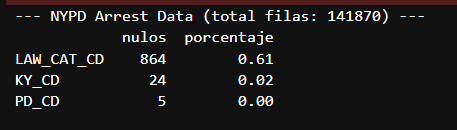
\includegraphics[width=\linewidth]{imagenes/image.png}\\[0.25cm]
        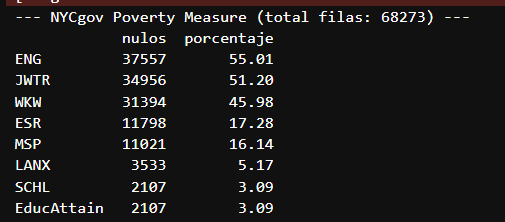
\includegraphics[width=\linewidth]{imagenes/image3.png}
    \end{minipage}\hfill
    \begin{minipage}[c]{0.50\textwidth}
        \centering
        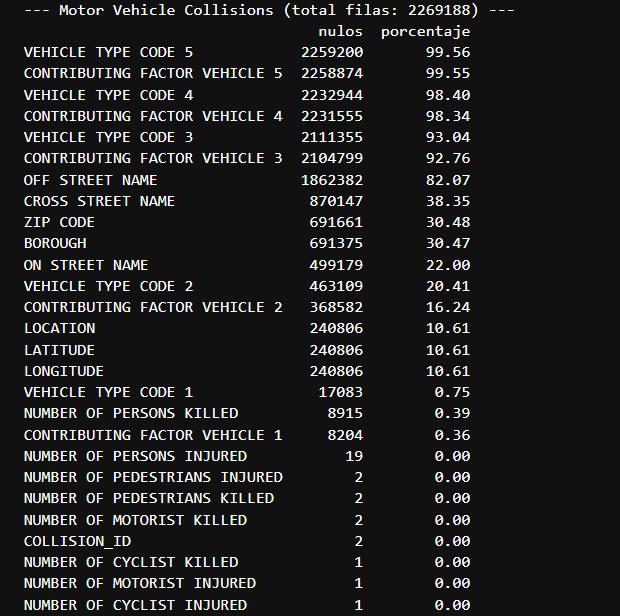
\includegraphics[width=\linewidth]{imagenes/image2.png}
    \end{minipage}
    \caption{Conteo y porcentaje de valores nulos en NYPD Arrest Data (izq. arriba), NYCgov Poverty Measure (izq. abajo) y Motor Vehicle Collisions (der.).}
    \label{fig:eda_elemento1_nulos}
\end{figure}

\subsection{Elemento 2 --- Estadísticos descriptivos generales}
\label{subsec:eda_elemento2}

Se calcularon estadísticos descriptivos distribuidos (conteo, media, desviación estándar, mínimo y máximo) mediante \texttt{.describe()} sobre variables numéricas clave de cada dataset. Para \textit{NYPD Arrest Data}, el precinto promedio de arresto es $63.41$ (desviación estándar de $34.01$, rango de $1$ a $123$), pero en las coordenadas planas estatales se detectó un mínimo anómalo de $-74$ en \texttt{X\_COORD\_CD} y de $40$ en \texttt{Y\_COORD\_CD}, valores que corresponden a latitud/longitud en grados decimales truncados y no a pies del sistema NAD 83. Para \textit{Motor Vehicle Collisions}, luego de aplicar conversión segura (\texttt{try\_cast}) sobre los conteos de víctimas, el promedio de personas heridas por colisión es $0.338$ ($\text{DE} = 0.722$, máximo $43$) y el de personas fallecidas es $0.00162$ ($\text{DE} = 0.0426$, máximo $8$).

\begin{figure}[H]
    \centering
    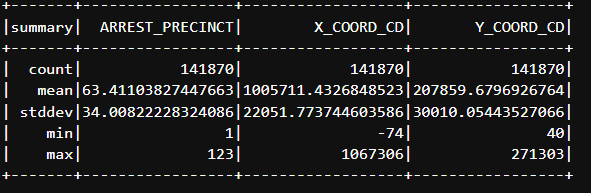
\includegraphics[width=0.75\textwidth]{imagenes/image4.png}\\[0.3cm]
    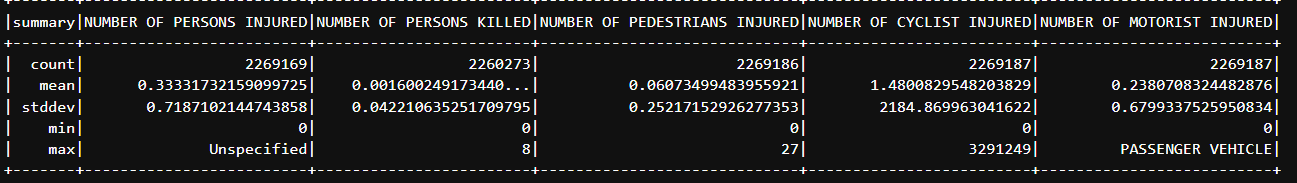
\includegraphics[width=0.95\textwidth]{imagenes/image5.png}
    \caption{Estadísticos descriptivos distribuidos (\texttt{.describe()}) para variables numéricas de arrestos y siniestros viales.}
    \label{fig:eda_elemento2_describe}
\end{figure}

\subsection{Elemento 3 --- Arrestos por Borough}
\label{subsec:eda_elemento3}

Brooklyn (\texttt{K}) concentra la mayor cantidad absoluta de arrestos con $42,877$ casos, seguido de Bronx (\texttt{B}) con $32,682$, Manhattan (\texttt{M}) con $32,089$, Queens (\texttt{Q}) con $29,053$ y, muy por debajo, Staten Island (\texttt{S}) con $5,169$. Esta distribución absoluta responde tanto al tamaño demográfico de cada condado como a la intensidad de patrullaje policial, motivo por el cual en la Sección \ref{sec:limpieza_transformacion} se estandariza por cada $100,000$ habitantes.

\begin{figure}[H]
    \centering
    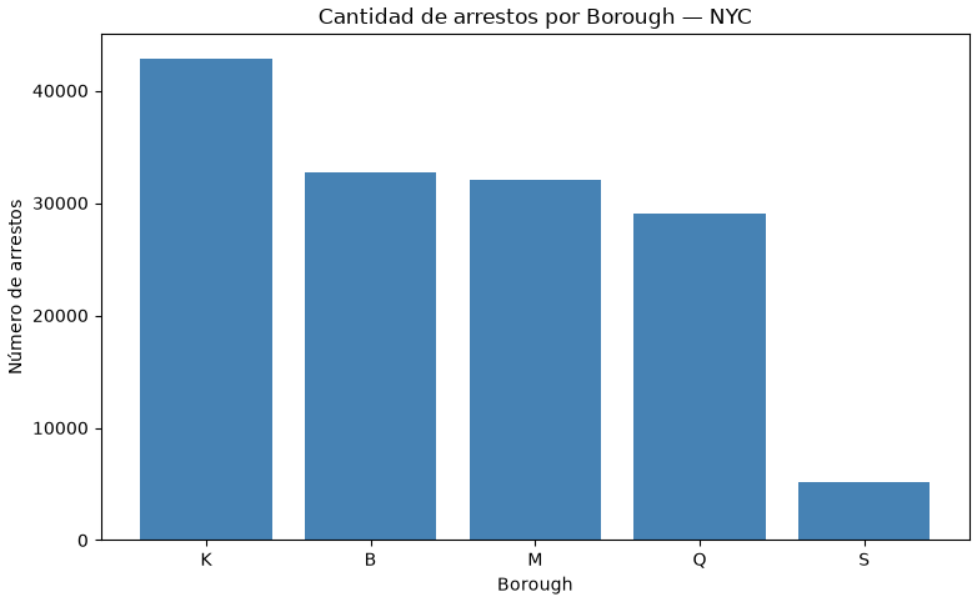
\includegraphics[width=0.75\textwidth]{imagenes/image6.png}
    \caption{Distribución absoluta de arrestos por condado (\textit{Borough}).}
    \label{fig:eda_elemento3_borough}
\end{figure}

\subsection{Elemento 4 --- Distribución de arrestos por nivel de gravedad de la ofensa}
\label{subsec:eda_elemento4}

El $58.5\%$ de los arrestos corresponden a delitos menores (\textit{misdemeanor}, \texttt{M}: $82,929$ casos), el $39.2\%$ a delitos graves (\textit{felony}, \texttt{F}: $55,651$ casos) y el $1.3\%$ a contravenciones (\textit{violation}, \texttt{V}: $1,896$ casos). Adicionalmente, se identificaron $864$ registros sin clasificación (\texttt{NaN}), $426$ registros con el código atípico \texttt{'9'}, $99$ con el código \texttt{'I'} (infracciones de tránsito/administrativas fuera de la tríada penal \texttt{F/M/V}) y $5$ con el texto \texttt{'(null)'}, sumando $1,394$ registros que se tratan en la fase de limpieza.

\begin{figure}[H]
    \centering
    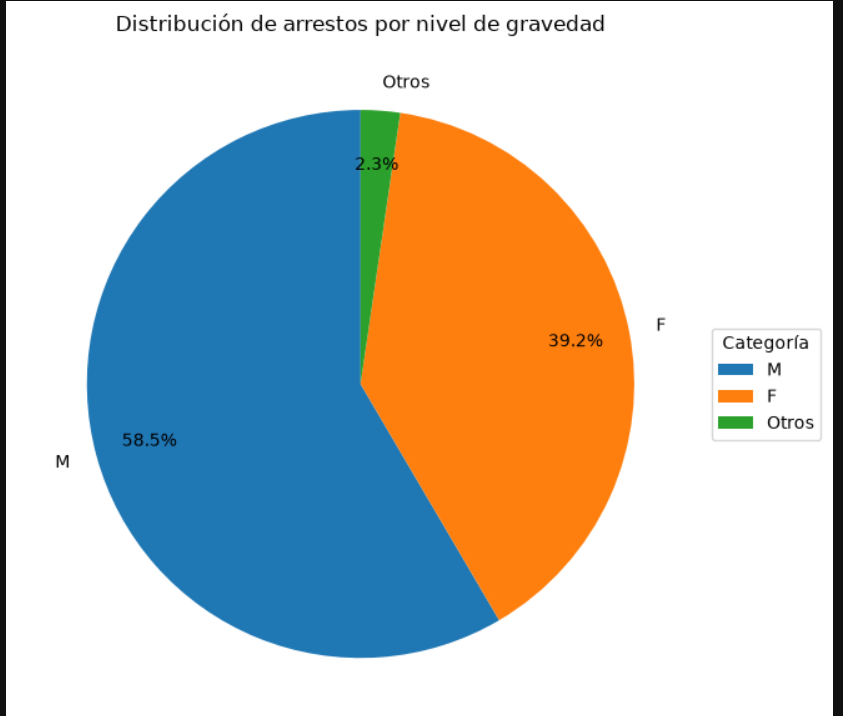
\includegraphics[width=0.75\textwidth]{imagenes/image7.png}
    \caption{Distribución de arrestos por nivel de gravedad de la ofensa (\texttt{LAW\_CAT\_CD}).}
    \label{fig:eda_elemento4_gravedad}
\end{figure}

\subsection{Elemento 5 --- Serie temporal de arrestos por mes}
\label{subsec:eda_elemento5}

Los arrestos mensuales muestran un comportamiento estable durante el primer semestre de 2026: enero registró $23,542$ detenciones, febrero presentó el punto más bajo ($21,069$, asociado también al menor número de días del mes), marzo subió a $24,696$, abril y mayo alcanzaron el máximo semestral prácticamente empatados ($25,129$ y $25,128$ respectivamente) y junio cerró en $22,306$ registros.

\begin{figure}[H]
    \centering
    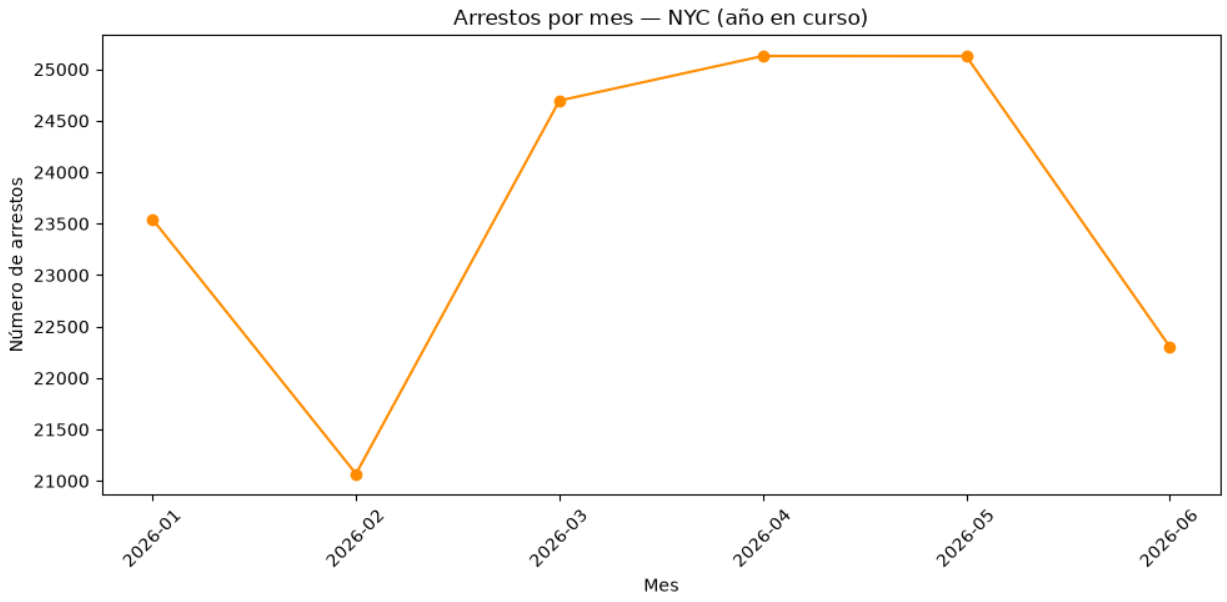
\includegraphics[width=0.70\textwidth]{imagenes/image8.png}
    \caption{Serie temporal mensual de arrestos en la Ciudad de Nueva York (enero a junio de 2026).}
    \label{fig:eda_elemento5_serie_temporal}
\end{figure}

\subsection{Elemento 6 --- Distribución de arrestos por grupo etario}
\label{subsec:eda_elemento6}

El grupo etario de \texttt{25-44} años concentra la mayoría de los arrestos con $81,521$ registros (equivalente al $57.46\%$ del total), seguido por el grupo de \texttt{45-64} años ($30,611$ registros, $21.58\%$) y el de \texttt{18-24} años ($20,946$ registros, $14.76\%$). Los extremos etarios (\texttt{<18} y \texttt{65+}) representan una proporción mucho menor ($5,587$ y $3,205$ arrestos, respectivamente).

\begin{figure}[H]
    \centering
    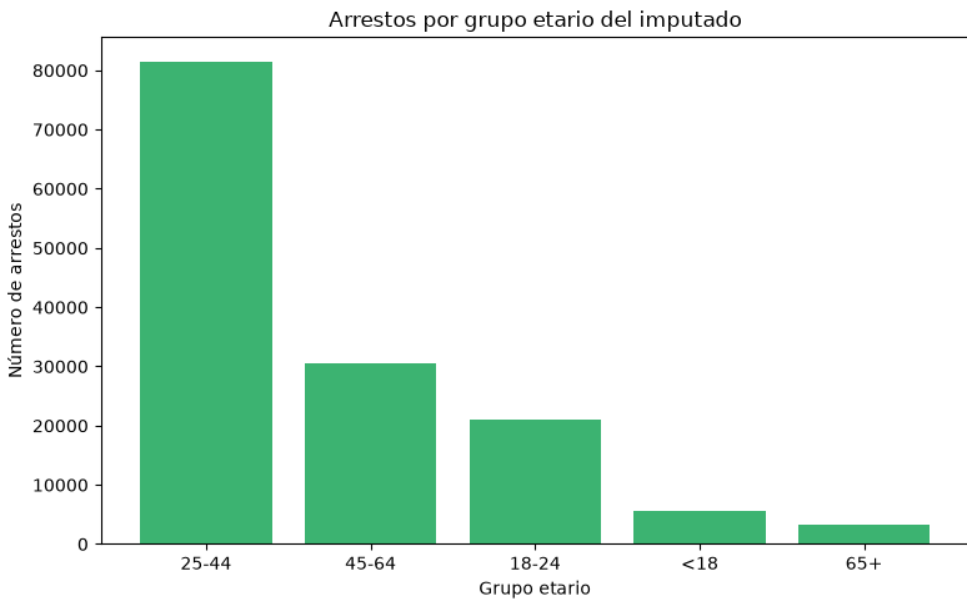
\includegraphics[width=0.65\textwidth]{imagenes/image9.png}
    \caption{Distribución de arrestos por grupo etario del imputado (\texttt{AGE\_GROUP}).}
    \label{fig:eda_elemento6_edad}
\end{figure}

\subsection{Elemento 7 --- Top 10 precincts con más arrestos}
\label{subsec:eda_elemento7}

El precinto $75$ (\textit{East New York}, Brooklyn) lidera el volumen de detenciones de toda la ciudad con $5,341$ arrestos, seguido del precinto $14$ (\textit{Midtown South}, Manhattan) con $4,382$ y el precinto $40$ (\textit{Mott Haven}, Bronx) con $4,061$. Completan los diez primeros lugares los precintos $46$ ($3,951$), $44$ ($3,882$), $103$ ($3,837$), $73$ ($3,524$), $52$ ($3,409$), $47$ ($3,084$) y $110$ ($3,001$), concentrados principalmente en el sur y centro del Bronx, el este de Brooklyn y el centro comercial de Manhattan.

\begin{figure}[H]
    \centering
    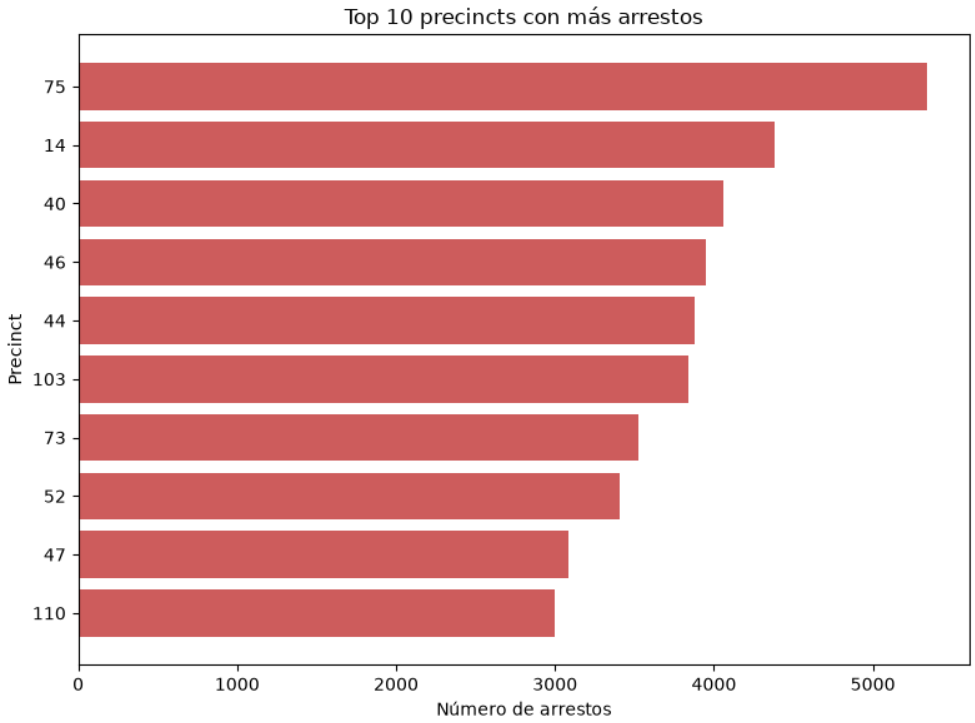
\includegraphics[width=0.75\textwidth]{imagenes/imagea.png}
    \caption{Top 10 distritos policiales (\textit{precincts}) con mayor volumen de arrestos.}
    \label{fig:eda_elemento7_top_precincts}
\end{figure}

\subsection{Elemento 8 --- Severidad de colisiones por tipo de persona involucrada (detección de registros desplazados)}
\label{subsec:eda_elemento8}

En la lectura exploratoria sin filtro de coherencia ni opción multilínea (Figura \ref{fig:eda_elemento8_severidad}), se detectó una anomalía crítica de calidad de datos: la suma de heridos por categoría superaba varias veces el total general de personas heridas debido a filas desplazadas por saltos de línea o comillas dentro de las direcciones, donde el identificador de colisión (\texttt{COLLISION\_ID} $\approx 3,291,249$) caía por error en la columna \texttt{NUMBER OF CYCLIST INJURED}. Este hallazgo motivó directamente la regla de lectura multilínea y el filtro de coherencia aritmética implementados en la Sección \ref{sec:limpieza_transformacion} (donde se presenta la distribución depurada real con $779,372$ heridos y $3,746$ fallecidos en la Figura \ref{fig:severidad_colisiones_limpia}).

\begin{figure}[H]
    \centering
    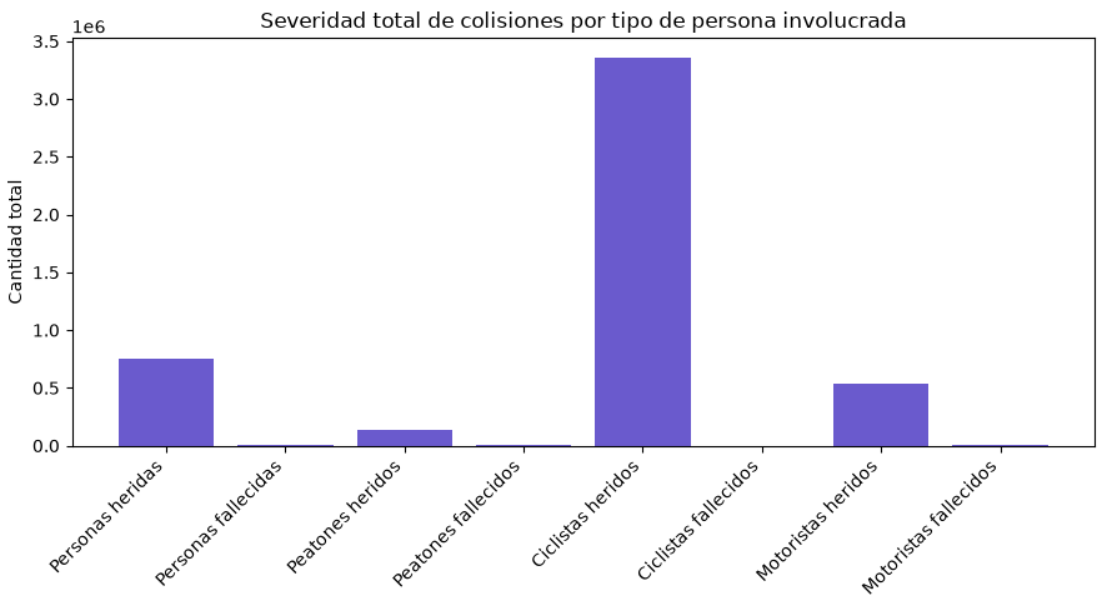
\includegraphics[width=0.85\textwidth]{imagenes/imageb.png}
    \caption{Inconsistencia detectada en la lectura preliminar de severidad de colisiones antes de aplicar el filtro de coherencia aritmética.}
    \label{fig:eda_elemento8_severidad}
\end{figure}

\subsection{Elemento 9 --- Cruce exploratorio entre tasa de pobreza y arrestos por Borough}
\label{subsec:eda_elemento9}

Al homologar los códigos de condado entre la encuesta de pobreza y los arrestos (Figura \ref{fig:eda_elemento9_pobreza_arrestos}), el Bronx presenta la mayor proporción muestral de pobreza ($25.79\%$), seguido de Brooklyn ($18.26\%$), Queens ($15.84\%$), y Manhattan y Staten Island ($13.83\%$ cada uno). En conteos brutos sin ponderar por población, Brooklyn registra más arrestos ($42,877$) que el Bronx ($32,682$); esta distorsión por tamaño poblacional se corrige en la Sección \ref{sec:limpieza_transformacion} mediante los factores de expansión \texttt{PWGTP}.

\begin{figure}[H]
    \centering
    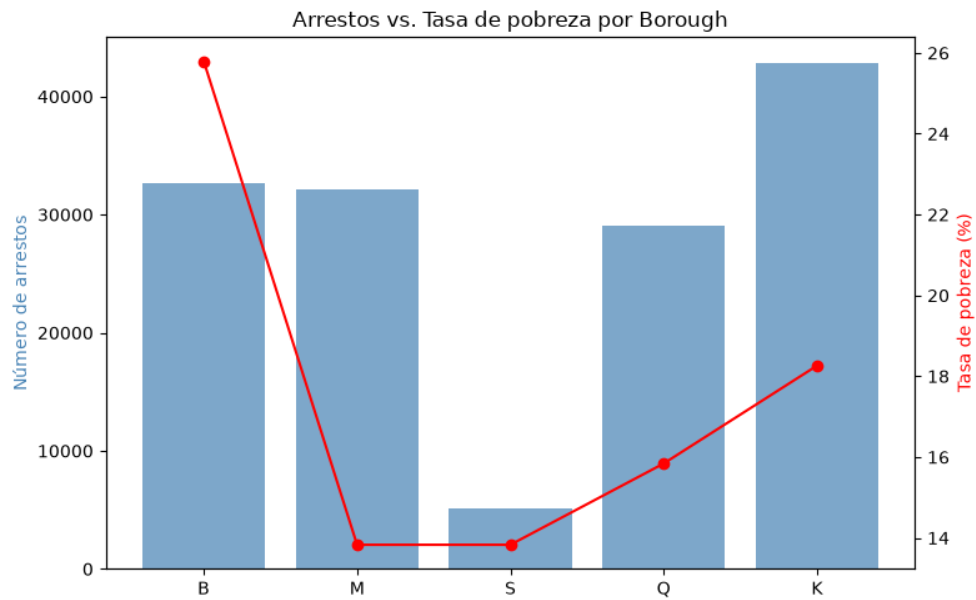
\includegraphics[width=0.8\textwidth]{imagenes/imagec.png}
    \caption{Cruce exploratorio inicial entre proporción muestral de pobreza y volumen bruto de arrestos por Borough.}
    \label{fig:eda_elemento9_pobreza_arrestos}
\end{figure}


\section{Reporte de Calidad de Datos}
\label{sec:reporte_calidad}

La evaluación rigurosa de la calidad de los datos garantiza que las respuestas a las preguntas de negocio y los modelos de aprendizaje automático en \textbf{Spark MLlib} no sufran sesgos por registros corruptos, duplicados o codificaciones inconsistentes. A continuación se sintetiza el diagnóstico de valores faltantes e inconsistencias detectadas en el clúster de Apache Spark y la estrategia técnica adoptada para cada caso.

\subsection{Conteo Distribuido de Valores Faltantes e Inconsistencias}
\label{subsec:conteo_faltantes}

\paragraph{A. Seguridad Ciudadana: NYPD Arrest Data ($141,870$ registros).}
Presenta una completitud superior al $99\%$ en sus atributos principales ($0\%$ de nulos en \texttt{ARREST\_KEY}, \texttt{ARREST\_DATE}, \texttt{ARREST\_BORO}, \texttt{ARREST\_PRECINCT}, \texttt{AGE\_GROUP}, \texttt{PERP\_SEX} y \texttt{PERP\_RACE}):
\begin{itemize}
    \item \textbf{\texttt{LAW\_CAT\_CD} (Nivel de gravedad de la ofensa):} $869$ valores nulos o equivalentes a texto vacío/\texttt{'(null)'} ($0.61\%$), a los que se suman $426$ registros con el código inválido \texttt{'9'} y $99$ registros con el código \texttt{'I'} (infracciones no clasificadas en \texttt{F/M/V}), totalizando $1,394$ registros ($0.98\%$) que requieren estandarización.
    \item \textbf{\texttt{PD\_DESC}, \texttt{OFNS\_DESC} y \texttt{KY\_CD}:} $24$ nulos cada uno ($0.02\%$).
    \item \textbf{\texttt{PD\_CD} y \texttt{LAW\_CODE}:} $5$ nulos cada uno ($0.00\%$).
    \item \textbf{Coordenadas planas (\texttt{X\_COORD\_CD}, \texttt{Y\_COORD\_CD}):} $9$ registros con coordenadas fuera del rango válido del plano estatal de Nueva York (valores truncados como $-74$ y $40$).
\end{itemize}

\paragraph{B. Siniestralidad Vial: Motor Vehicle Collisions ($2,305,623$ registros crudos).}
Presenta tres familias diferenciadas de problemas de calidad:
\begin{itemize}
    \item \textbf{Nulos estructurales en vehículos secundarios (3, 4 y 5):} \texttt{VEHICLE TYPE CODE 5} ($2,295,439$ nulos, $99.56\%$), \texttt{CONTRIBUTING FACTOR VEHICLE 5} ($2,295,099$, $99.54\%$), \texttt{VEHICLE TYPE CODE 4} ($2,268,679$, $98.40\%$), \texttt{CONTRIBUTING FACTOR VEHICLE 4} ($2,267,226$, $98.33\%$), \texttt{VEHICLE TYPE CODE 3} ($2,145,137$, $93.04\%$) y \texttt{CONTRIBUTING FACTOR VEHICLE 3} ($2,138,209$, $92.74\%$). En el vehículo 2 los nulos son del $20.62\%$ y $16.24\%$, y en el vehículo 1 apenas del $0.77\%$ ($17,718$) y $0.36\%$ ($8,228$).
    \item \textbf{Faltantes de geocodificación y etiquetas administrativas:} \texttt{CROSS STREET NAME} ($81.85\%$), \texttt{OFF STREET NAME} ($38.48\%$), \texttt{ZIP CODE} ($701,201$ nulos, $30.41\%$), \texttt{BOROUGH} ($674,935$ nulos, $29.27\%$) y \texttt{LATITUDE}/\texttt{LONGITUDE} ($240,776$ nulos, $10.44\%$, más $8,566$ puntos con coordenadas $(0,0)$ o fuera del rectángulo geográfico de NYC).
    \item \textbf{Registros corruptos, conteos incoherentes y separador decimal local:} $268$ registros presentan desplazamientos de columnas, conteos nulos en \texttt{NUMBER OF PERSONS KILLED} ($31$) o \texttt{INJURED} ($18$), llaves duplicadas o sumas de subcategorías mayores al total de víctimas; además, las columnas \texttt{LATITUDE} y \texttt{LONGITUDE} almacenan decimales con coma (\texttt{'40,62179'}).
\end{itemize}

\paragraph{C. Determinantes Socioeconómicos: NYCgov Poverty Measure ($68,273$ registros).}
La ausencia de datos obedece al diseño de salto lógico (\textit{skip logic}) del cuestionario censal ACS:
\begin{itemize}
    \item \textbf{\texttt{ENG} (Dominio del inglés):} $37,557$ nulos ($55.01\%$, personas que solo hablan inglés en casa).
    \item \textbf{\texttt{JWTR} (Medio de transporte al trabajo):} $34,956$ nulos ($51.20\%$, personas que no trabajaron la semana previa).
    \item \textbf{\texttt{WKW} (Semanas trabajadas):} $31,394$ nulos ($45.98\%$).
    \item \textbf{\texttt{ESR} (Estatus de empleo) y \texttt{MSP} (Estado civil):} $11,798$ ($17.28\%$) y $11,021$ ($16.14\%$) nulos (menores de 15 o 16 años a quienes no aplica la pregunta).
    \item \textbf{\texttt{LANX} ($5.17\%$) y \texttt{SCHL}/\texttt{EducAttain} ($3.09\%$):} Menores de 3 o 5 años fuera del universo escolar.
\end{itemize}

\subsection{Estrategia Técnica Implementada para el Tratamiento de Calidad}
\label{subsec:tecnicas_faltantes}

Descartar por completo cualquier fila con algún campo nulo (\textit{list-wise deletion}) habría eliminado más del $99\%$ de las colisiones vehiculares y más del $55\%$ de la encuesta socioeconómica. Por ello, en el pipeline de PySpark (documentado y ejecutado en la Sección \ref{sec:limpieza_transformacion}) se adoptaron cuatro mecanismos específicos:

\begin{enumerate}
    \item \textbf{Validación Geoespacial por Caja Delimitadora y Malla Regular de $0.01^\circ \times 0.01^\circ$:} Dado que el $29.27\%$ de las colisiones carece de la etiqueta \texttt{BOROUGH} pero el $89.19\%$ ($2,056,013$ siniestros) posee coordenadas geográficas válidas dentro de Nueva York ($\text{lat} \in [40.49^\circ, 40.92^\circ]$, $\text{lon} \in [-74.27^\circ, -73.68^\circ]$), se creó el indicador booleano \texttt{coord\_valida} y se discretizó el territorio en cuadrículas uniformes de $0.01^\circ \times 0.01^\circ$ ($\approx 1.1\text{ km} \times 0.85\text{ km}$) usando funciones nativas de PySpark (\texttt{F.floor(lat * 100)}). Esto permitió realizar el cruce espacial entre colisiones y arrestos y entrenar los modelos de MLlib conservando el $100\%$ de los eventos válidamente georreferenciados sin depender de extensiones externas ni imputar artificialmente el condado en análisis administrativos.
    \item \textbf{Imputación Jerárquica por Moda Condicionada (\texttt{Window.partitionBy}):} Para los $1,394$ registros de arrestos sin categoría penal válida en \texttt{LAW\_CAT\_CD}, en lugar de aplicar únicamente una moda global ciega, se calculó en PySpark la moda de \texttt{LAW\_CAT\_CD} dentro de cada código específico de delito (\texttt{PD\_CD}) mediante una ventana particionada, usando la moda global (\texttt{M}) solo como respaldo cuando el \texttt{PD\_CD} también era nulo. Además, se preservó la columna \texttt{gravedad\_reportada} sin imputar para garantizar total transparencia en las consultas descriptivas por gravedad.
    \item \textbf{Codificación Explícita de Ausencia Estructural (\textit{Missing Indicators}):} En las columnas de los vehículos 3, 4 y 5 de colisiones se asignó la categoría explícita \texttt{SIN\_VEHICULO\_3}, \texttt{SIN\_VEHICULO\_4} y \texttt{SIN\_VEHICULO\_5}, y en las variables numéricas con salto lógico de la encuesta de pobreza (\texttt{ENG}, \texttt{JWTR}, \texttt{WKW}, \texttt{ESR}, \texttt{MSP}, \texttt{LANX}) se asignó el código centinela $-1$ (\textit{``no aplica''}), reduciendo a $0$ los valores nulos en dichas columnas.
    \item \textbf{Estandarización de Separadores Numéricos y Filtrado de Integridad:} Se convirtieron las comas decimales y puntos de miles en coordenadas e importes monetarios mediante expresiones regulares distribuidas (\texttt{try\_cast(replace(...))}), descartando únicamente los $268$ registros de colisiones con llaves ausentes, duplicadas o conteos de víctimas aritméticamente imposibles.
\end{enumerate}


\section{Planteamiento de Preguntas de Negocio sobre los Datos}
\label{sec:preguntas_negocio}

Para guiar la extracción de conocimiento y el modelado en \textbf{Spark MLlib} en línea con los tres objetivos de negocio del proyecto (\textit{NYPD}, \textit{NYC DOT Vision Zero} y \textit{NYC Opportunity}), se formularon ocho preguntas directrices de negocio. Todas ellas se resuelven cuantitativa y visualmente en las Secciones \ref{sec:respuestas_preguntas} y \ref{sec:modelado_evaluacion}:

\begin{enumerate}

    \item \textbf{¿Cómo varía la concentración espacial y temporal de los arrestos por delitos graves (felonías) a lo largo del ciclo semanal en los distintos condados de Nueva York?}\\
    \textit{Justificación de negocio (Objetivo 1 --- NYPD):} Dado que los registros abiertos de arrestos del NYPD informan la fecha exacta del evento con granularidad diaria (\texttt{ARREST\_DATE}), caracterizar cómo se distribuyen las felonías (\texttt{LAW\_CAT\_CD = 'F'}) entre los días de la semana (lunes a domingo y días laborales frente a fin de semana) en cada uno de los cinco condados permite identificar los picos operativos de actividad criminal y optimizar la programación semanal de patrullas y unidades tácticas.

    \item \textbf{¿Existe una correlación significativa entre los condados con mayor índice de pobreza ponderada y el volumen o la tasa de arrestos por delitos menores?}\\
    \textit{Justificación de negocio (Objetivos 1 y 3 --- NYPD y NYC Opportunity):} Busca contrastar empíricamente si las detenciones por delitos menores (\textit{misdemeanors}, \texttt{M}) se asocian a nivel de condado con la proporción de población en pobreza (\texttt{NYCgov\_Pov\_Stat = 1} ponderada con \texttt{PWGTP}), tanto en conteos absolutos como en tasas por cada $100,000$ habitantes, orientando el balance entre políticas de prevención social y control policial.

    \item \textbf{En el marco de la iniciativa \textit{Vision Zero}, ¿cuáles son los factores contribuyentes y los tipos de vehículos más frecuentes en las colisiones que resultan en peatones o ciclistas heridos o fallecidos?}\\
    \textit{Justificación de negocio (Objetivo 2 --- NYC DOT Vision Zero):} Aislar las causas conductuales (distracción, no ceder el paso, velocidad) y las tipologías vehiculares (SUV, sedanes, transporte comercial) involucradas en siniestros con actores viales vulnerables provee evidencia directa para focalizar controles de tránsito y rediseño de intersecciones.

    \item \textbf{¿Qué relación guardan las condiciones socioeconómicas de desempleo y nivel educativo alcanzado con las tasas de siniestralidad vial fatal por cada $100,000$ habitantes en los cinco condados?}\\
    \textit{Justificación de negocio (Objetivos 2 y 3 --- Vision Zero y NYC Opportunity):} Cruzar la tasa ponderada de desempleo civil (\texttt{ESR}) y la distribución de escolaridad en mayores de 25 años (\texttt{SCHL}) con la tasa de colisiones mortales por cada $100,000$ habitantes permite evaluar si la letalidad vial a escala macro de condado responde a brechas socioeconómicas o a dinámicas de exposición vial e infraestructura arterial.

    \item \textbf{¿Cuáles son las cinco ``zonas calientes duales'' (\textit{hotspots}) donde coinciden geográficamente la mayor concentración de arrestos y de colisiones de tránsito fatales?}\\
    \textit{Justificación de negocio (Objetivos 1 y 2 --- Intervención Conjunta Alcaldía):} Identificar a alta resolución espacial (cuadrículas de $0.01^\circ \times 0.01^\circ$) los cinco microterritorios que encabezan simultáneamente el percentil de detenciones y de siniestros mortales permite a la Alcaldía focalizar presupuestos integrados (iluminación, cámaras, señalización y patrullaje) con doble retorno social.

    \item \textbf{¿Cuál es el perfil demográfico predominante (grupo etario, sexo y raza registrada) de los individuos arrestados según el nivel de severidad del delito (Contravención, Delito Menor y Felonía)?}\\
    \textit{Justificación de negocio (Objetivos 1 y 3 --- NYPD y Política Social):} Caracterizar la composición demográfica de las detenciones en las categorías \texttt{V}, \texttt{M} y \texttt{F} permite identificar los grupos poblacionales con mayor incidencia en los registros policiales y diseñar programas focalizados de prevención comunitaria.

    \item \textbf{¿Cómo difiere el comportamiento horario y la frecuencia de los accidentes de tránsito en un condado de altísima densidad comercial (Manhattan) frente a un condado de carácter residencial y suburbano (Staten Island)?}\\
    \textit{Justificación de negocio (Objetivo 2 --- Gestión de Tráfico NYC DOT):} Comparar tanto el volumen horario absoluto como la curva porcentual intradiaria de siniestros entre Manhattan y Staten Island permite cuantificar el impacto de la población flotante y ajustar de forma asimétrica los planes de semaforización y agentes de tránsito.

    \item \textbf{¿Qué variables (hora del día, coordenadas geográficas, tipo de vehículo y factor contribuyente) se asocian en mayor medida con la probabilidad de que un accidente vehicular resulte en fatalidad dentro de un modelo de aprendizaje automático en Spark MLlib?}\\
    \textit{Justificación de negocio (Objetivo 2 --- Núcleo Predictivo en MLlib):} Constituye el puente entre las preguntas de negocio y la fase de modelado supervisado, permitiendo cuantificar la capacidad discriminativa de los atributos reportados en el formulario MV-104AN y el peso relativo de cada familia de predictores sobre el riesgo de muerte vial.

\end{enumerate}


% --- SECCIONES MODULARES: ENTREGA FINAL (FASES III, IV, V Y VI CRISP-DM) ---
\section{Filtros, Limpieza y Transformaciones Finales}
\label{sec:limpieza_transformacion}

De acuerdo con los requisitos de la entrega final, una vez consolidado el entendimiento del negocio y de los datos, se culminó el pipeline de limpieza, filtrado y transformación distribuida en \textbf{Apache Spark} (\texttt{spark://10.195.34.34:7077}). El diseño se estructuró en tres capas de datos en memoria: (i) \textit{datos de origen} (\texttt{df\_arrests}, \texttt{df\_col\_raw}, \texttt{df\_poverty}), que preservan los registros recibidos para auditar esquemas y nulos; (ii) \textit{datos depurados} (\texttt{arr\_dep}, \texttt{col\_dep}, \texttt{pov\_dep}), sobre los cuales se aplican las reglas de filtrado de integridad; y (iii) \textit{datos para análisis y modelado} (\texttt{arr\_analisis}, \texttt{col\_analisis}, \texttt{pov\_analisis}), enriquecidos con las transformaciones e imputaciones requeridas para responder las preguntas de negocio y entrenar los modelos en \textbf{Spark MLlib}.

\subsection{Filtros Aplicados y su Justificación Técnica y de Negocio}
\label{subsec:filtros_inconsistentes}

Se implementaron \textbf{cuatro filtros principales} sobre los DataFrames de Spark (superando el mínimo de dos filtros exigido), complementados con un filtro lógico no destructivo para coordenadas geoespaciales (\texttt{coord\_valida}). La Tabla \ref{tab:reglas_filtrado} detalla cada regla y su justificación.

\begin{table}[H]
\centering
\scriptsize
\renewcommand{\arraystretch}{1.25}
\caption{Reglas finales de filtrado implementadas en PySpark y su justificación.}
\label{tab:reglas_filtrado}
\begin{tabularx}{\linewidth}{c l >{\raggedright\arraybackslash}p{3.6cm} >{\raggedright\arraybackslash}p{4.2cm} X}
\toprule
\textbf{\#} & \textbf{Dataset} & \textbf{Problema detectado} & \textbf{Filtro aplicado en PySpark} & \textbf{Justificación técnica y de negocio} \\
\midrule
F1 & Collisions & Filas desplazadas por saltos de línea, llave ausente o conteos no convertibles / negativos en las 8 columnas \texttt{NUMBER OF...} & Lectura con \texttt{multiLine=True}, \texttt{quote}, \texttt{escape}; \texttt{COLLISION\_ID.isNotNull() \& length > 0} y \texttt{try\_cast(c AS INT) >= 0} en las 8 columnas de víctimas. & Garantiza que cada registro represente un evento vial real y elimina corrupciones de parseo (p.\,ej., el valor espurio de $3,291,249$ en ciclistas heridos detectado en el EDA). \\
F2 & Collisions & Incoherencia aritmética entre subcategorías y el total de víctimas del choque & \texttt{(PEDESTRIANS + CYCLIST + MOTORIST INJURED) <= PERSONS INJURED} (e idéntica condición para \texttt{KILLED}). & Peatones, ciclistas y motoristas son subconjuntos disjuntos del total de personas afectadas; violar esta desigualdad altera las tasas de letalidad de \textit{Vision Zero}. \\
F3 & Collisions \& Arrests & Duplicidad de registros de eventos por llave primaria & \texttt{dropDuplicates(['COLLISION\_ID'])} en colisiones y \texttt{ARREST\_KEY.isNotNull()} con \texttt{dropDuplicates(['ARREST\_KEY'])} en arrestos. & Previene el doble conteo de detenciones o siniestros viales en las agregaciones territoriales y en el entrenamiento supervisado. \\
F4 & Poverty & Factores de expansión muestral nulos o no positivos & \texttt{filter(F.col('PWGTP') > 0)} sobre los microdatos socioeconómicos. & Las estimaciones ponderadas de población, pobreza y desempleo exigen pesos muestrales estrictamente positivos como denominador. \\
\bottomrule
\end{tabularx}
\end{table}

\subsubsection{Evidencia Cuantitativa de los Filtros (Conteos Antes y Después)}

La Tabla \ref{tab:conteos_filtros} reporta el resultado exacto de la ejecución distribuida de los filtros F1 a F4 sobre el clúster de Spark, junto con la evaluación del indicador de calidad espacial \texttt{coord\_valida} (definido como $\text{lat} \in [40.49^\circ, 40.92^\circ]$ y $\text{lon} \in [-74.27^\circ, -73.68^\circ]$ en colisiones, y $X \in [900{,}000, 1{,}070{,}000]$, $Y \in [110{,}000, 275{,}000]$ pies NAD 83 en arrestos). Conservar los registros con \texttt{coord\_valida = False} en la tabla general y filtrarlos únicamente en las consultas geoespaciales evita perder información válida en los análisis temporales y categóricos.

\begin{table}[H]
\centering
\scriptsize
\renewcommand{\arraystretch}{1.2}
\caption{Conteo de registros antes y después de los filtros de integridad y validación espacial en Spark.}
\label{tab:conteos_filtros}
\resizebox{\textwidth}{!}{%
\begin{tabular}{l r r r r r}
\toprule
\textbf{Conjunto de Datos} & \textbf{Registros antes} & \textbf{Registros después} & \textbf{Descartados} & \textbf{\texttt{coord\_valida = True}} & \textbf{\texttt{coord\_valida = False}} \\
\midrule
NYPD Arrest Data & 141,870 & 141,870 & 0 & 141,861 (99.99\%) & 9 (0.01\%) \\
Motor Vehicle Collisions & 2,305,623 & 2,305,355 & 268 & 2,056,013 (89.18\%) & 249,342 (10.82\%) \\
NYCgov Poverty Measure & 68,273 & 68,273 & 0 & N/A (nivel \texttt{Boro}) & N/A \\
\bottomrule
\end{tabular}%
}
\end{table}

\subsection{Transformaciones Finales y su Justificación}
\label{subsec:limpieza_datos}

Sobre los datos depurados se aplicaron \textbf{seis transformaciones distribuidas} (superando ampliamente el mínimo de tres transformaciones requerido), resumidas en la Tabla \ref{tab:transformaciones_finales}.

\begin{table}[H]
\centering
\scriptsize
\renewcommand{\arraystretch}{1.25}
\caption{Transformaciones finales implementadas sobre los DataFrames en Apache Spark.}
\label{tab:transformaciones_finales}
\begin{tabularx}{\linewidth}{c l >{\raggedright\arraybackslash}p{4.3cm} X}
\toprule
\textbf{\#} & \textbf{Dataset} & \textbf{Transformación implementada} & \textbf{Justificación técnica y de negocio} \\
\midrule
T1 & Todos & \textbf{Conversión de separadores numéricos y tipos:} Reemplazo de coma decimal por punto en coordenadas (\texttt{replace(LATITUDE, ',', '.')}) y limpieza de puntos de miles y comas decimales en las $22$ columnas monetarias de pobreza (\texttt{EST\_*}, \texttt{*\_adj}, \texttt{NYCgov\_Income}, \texttt{NYCgov\_Threshold}, \texttt{PreTaxIncome\_PU}) antes de aplicar \texttt{try\_cast(... AS DOUBLE)}. & Los archivos CSV utilizan convención numérica local; sin esta transformación, el motor infiere las coordenadas y los ingresos como texto (\texttt{StringType}) o produce \texttt{NULL} al convertirlos directamente. \\
T2 & Arrests \& Collisions & \textbf{Estandarización temporal y textual:} Conversión de \texttt{ARREST\_DATE} y \texttt{CRASH DATE} a \texttt{DateType} (\texttt{MM/dd/yyyy}), extracción de la hora entera $\texttt{hora} \in \{0,\dots,23\}$ desde \texttt{CRASH TIME} (\texttt{H:mm}), e higienización textual (\texttt{F.upper(F.trim(...))}) en descripciones delictivas, calles, vehículos y factores. & Habilita el particionamiento temporal por año/semestre, el análisis horario de siniestralidad y elimina categorías duplicadas por diferencias de mayúsculas o espacios en blanco. \\
T3 & Arrests & \textbf{Depuración de catálogo e imputación jerárquica de \texttt{LAW\_CAT\_CD} por moda condicionada:} Preservación de la columna original en \texttt{gravedad\_reportada}; recodificación a \texttt{NULL} de valores fuera de \texttt{\{F, M, V\}} (\texttt{'9'}, \texttt{'I'}, \texttt{'(null)'}) e imputación de los $1,394$ nulos mediante la moda de \texttt{LAW\_CAT\_CD} particionada por código interno de delito (\texttt{Window.partitionBy('PD\_CD')}), con respaldo en la moda global (\texttt{M}). & Dado que cada código interno \texttt{PD\_CD} tipifica un delito específico, imputar según la moda de su propio \texttt{PD\_CD} preserva la correspondencia jurídica real (dejando $0$ nulos), mientras que conservar \texttt{gravedad\_reportada} evita alterar los conteos descriptivos de las preguntas 1, 2 y 6. \\
T4 & Collisions \& Poverty & \textbf{Codificación explícita de nulos estructurales:} Asignación de la etiqueta \texttt{SIN\_VEHICULO\_3..5} en los tipos y factores de vehículos 3 a 5 de colisiones, y del código centinela $-1$ en \texttt{ENG}, \texttt{JWTR}, \texttt{WKW}, \texttt{ESR}, \texttt{MSP} y \texttt{LANX} de pobreza, más normalización de \texttt{AGE\_GROUP} fuera de catálogo a \texttt{DESCONOCIDO}. & Distingue la ausencia estructural (choques con menos de 3 vehículos o saltos lógicos del cuestionario censal) de la pérdida accidental de información, logrando $0$ nulos en todas las variables tratadas. \\
T5 & Todos & \textbf{Armonización interinstitucional de condados (\texttt{BORO}) y cálculo de tasas por $100,000$ habitantes:} Homologación de códigos numéricos (\texttt{1..5} en pobreza) y alfabéticos (\texttt{B, K, M, Q, S} en arrestos) al nombre estándar en mayúsculas (\texttt{BRONX, BROOKLYN, MANHATTAN, QUEENS, STATEN ISLAND}) y cálculo de tasas dividiendo por la población expandida $\sum \texttt{PWGTP}$. & Permite cruzar los tres conjuntos de datos y comparar condados de tamaños demográficos muy dispares (desde $469,393$ hab. en Staten Island hasta $2,540,638$ hab. en Brooklyn) bajo una métrica epidemiológica y criminológica estándar. \\
T6 & Collisions \& Arrests & \textbf{Ingeniería de características espaciales y matemáticas para MLlib:} Discretización en cuadrículas de $0.01^\circ \times 0.01^\circ$ ($\texttt{x} = \lfloor \texttt{lon}\times 100\rfloor$, $\texttt{y} = \lfloor \texttt{lat}\times 100\rfloor$), codificación cíclica de la hora ($\sin(2\pi h/24)$, $\cos(2\pi h/24)$), transformación logarítmica $\log(1+x)$ de conteos por zona e indicadores binarios de fatalidad y afectación a vulnerables. & Provee las variables de entrada estandarizadas para el ranking espacial (Pregunta 5), la Regresión Logística, el agrupamiento K-Means y la Red Neuronal Profunda. \\
\bottomrule
\end{tabularx}
\end{table}

\subsubsection{Resultados de la Transformación T5: Tasas Estandarizadas por 100,000 Habitantes}

Al expandir la muestra de \textit{NYCgov Poverty Measure} mediante la suma del peso personal \texttt{PWGTP} por condado y cruzarla con los arrestos acumulados del semestre y las colisiones con condado informado del último año completo de referencia ($2025$), se obtiene la Tabla \ref{tab:tasas_100k} y la Figura \ref{fig:tasas_100k}.

\begin{table}[H]
\centering
\small
\renewcommand{\arraystretch}{1.2}
\caption{Población estimada (\texttt{PWGTP}) y tasas estandarizadas de arrestos y colisiones por cada 100,000 habitantes.}
\label{tab:tasas_100k}
\resizebox{\textwidth}{!}{%
\begin{tabular}{l r r r r r}
\toprule
\textbf{Condado (\texttt{BORO})} & \textbf{Población est. (\texttt{PWGTP})} & \textbf{Arrestos} & \textbf{Colisiones (2025)} & \textbf{Arrestos / 100k} & \textbf{Colisiones / 100k} \\
\midrule
BRONX & 1,388,068.2 & 32,682 & 12,291 & \textbf{2,354.5} & 885.5 \\
MANHATTAN & 1,554,658.6 & 32,089 & 14,488 & 2,064.1 & 931.9 \\
BROOKLYN & 2,540,638.0 & 42,877 & 26,712 & 1,687.6 & \textbf{1,051.4} \\
QUEENS & 2,250,749.0 & 29,053 & 21,840 & 1,290.8 & 970.3 \\
STATEN ISLAND & 469,393.0 & 5,169 & 3,128 & 1,101.2 & 666.4 \\
\bottomrule
\end{tabular}%
}
\end{table}

\begin{figure}[H]
    \centering
    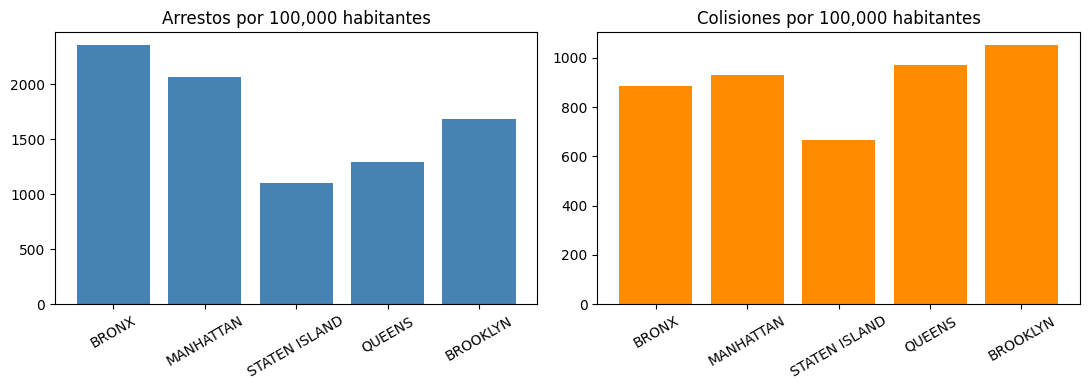
\includegraphics[width=0.92\textwidth]{imagenes/fig_cell_43_1.png}
    \caption{Comparación de tasas estandarizadas de arrestos y colisiones por cada 100,000 habitantes entre los cinco condados.}
    \label{fig:tasas_100k}
\end{figure}

\noindent \textbf{Hallazgo clave de la estandarización:} Mientras que en cifras brutas Brooklyn ocupaba el primer lugar en arrestos ($42,877$), al normalizar por la población estimada de cada condado \textbf{El Bronx pasa a encabezar la tasa de detenciones con $2,354.5$ arrestos por cada $100,000$ habitantes}, seguido de Manhattan ($2,064.1$, influenciado por su alta población flotante) y desplazando a Brooklyn al tercer lugar ($1,687.6$). En contraste, en siniestralidad vial de 2025, \textbf{Brooklyn mantiene el primer lugar tanto en volumen absoluto ($26,712$) como en tasa relativa ($1,051.4$ colisiones por cada $100,000$ habitantes)}, seguido por Queens ($970.3$).

\subsubsection{Verificación de Severidad Vial tras el Filtrado de Integridad (Elemento 8 Depurado)}

Una vez aplicados los filtros F1, F2 y F3 sobre el histórico de colisiones ($2,305,355$ registros limpios), se recalculó la distribución acumulada de heridos y fallecidos por tipo de actor vial (Figura \ref{fig:severidad_colisiones_limpia}). Se verifica la eliminación total de la distorsión detectada en la exploración preliminar: el histórico limpio registra exactamente \textbf{$779,372$ personas heridas} y \textbf{$3,746$ personas fallecidas}. Los ocupantes de vehículos motorizados concentran el mayor volumen de heridos ($552,978$, seguidos de $141,625$ peatones y $68,866$ ciclistas), pero \textbf{los peatones concentran la mayor cantidad de víctimas mortales ($1,847$ fallecidos, equivalentes al $49.3\%$ del total de muertes viales)}, superando a los motoristas ($1,484$) y ciclistas ($273$).

\begin{figure}[H]
    \centering
    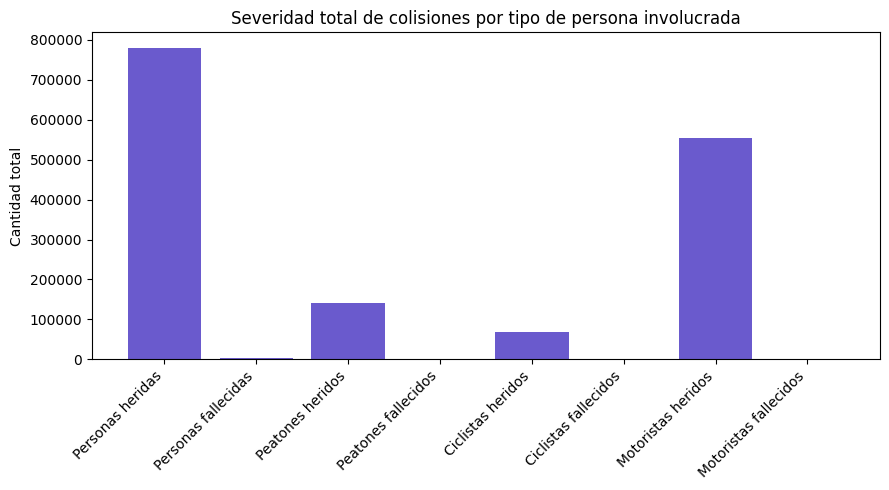
\includegraphics[width=0.78\textwidth]{imagenes/fig_cell_46_1.png}
    \caption{Severidad total acumulada de colisiones por tipo de persona involucrada sobre el conjunto depurado ($2,305,355$ siniestros).}
    \label{fig:severidad_colisiones_limpia}
\end{figure}


\section{Enriquecimiento Analítico: Web Scraping de Salud Pública y API Climática}
\label{sec:bonos}

Esta sección documenta la integración de las dos fuentes externas de enriquecimiento territorial y ambiental (previstas en el numeral 2.4 y conectadas en Spark con los conjuntos principales de arrestos, colisiones y pobreza): la extracción automatizada de tasas de incidencia de cáncer por vecindario mediante \textit{web scraping} del \textit{NYS Department of Health} y la extracción de series meteorológicas diarias mediante API REST (\textit{OpenWeather One Call 3.0 / Open-Meteo}).

\subsection{Web Scraping: Tasas de Cáncer por Vecindario PUMA (NYS Department of Health)}
\label{subsec:bono_cancer}

La fuente consultada es el tablero oficial \textit{``Rate by PUMA''} del \textit{New York State Cancer Registry} \cite{nys_cancer_registry_2026}, donde los vecindarios de Nueva York se delimitan mediante unidades censales PUMA (\textit{Public Use Microdata Areas}), equivalentes aproximadamente a los distritos comunitarios de la ciudad. Dado que la página institucional incrusta una vista dinámica de \textit{Tableau Public} en lugar de una tabla HTML estática, el flujo programado en Python ejecuta cuatro etapas: (i) descarga el documento HTML de \texttt{ratebyPUMA.htm} mediante \texttt{requests}, (ii) identifica mediante expresiones regulares la ruta del libro (\texttt{cancerstatisticreportcounty}) y la hoja (\texttt{7\_RatebyPUMA}) a partir de los metadatos de vista previa de Tableau, (iii) descarga directamente el flujo CSV subyacente desde el servidor de \textit{Tableau Public} y (iv) normaliza las columnas para conservar la serie agregada (\textit{All Sites Combined}, ambos sexos) para cada uno de los $55$ PUMA de la Ciudad de Nueva York, almacenando además una copia en caché local (\texttt{cancer\_tasas\_puma\_nyc.csv}) para garantizar reproducibilidad en entornos de clúster con acceso restringido.

\subsection{Resultados del Scraping: Distribución de Tasas por PUMA y Condado}
\label{subsec:bono_puma}

Se extrajeron exitosamente los registros de los $55$ PUMA de la metrópoli ($10$ en el Bronx, $18$ en Brooklyn, $10$ en Manhattan, $14$ en Queens y $3$ en Staten Island). La tasa promedio de incidencia en los vecindarios de la ciudad es de $423.5$ casos por cada $100,000$ habitantes, con un rango entre $355.7$ (\textit{Bushwick}, Brooklyn) y $541.0$ (\textit{South Shore}, Staten Island). La Tabla \ref{tab:top10_puma_cancer} presenta los diez vecindarios con mayor tasa y la Figura \ref{fig:bono_cancer_puma} ilustra la dispersión intraterritorial por condado junto con el ranking de los diez primeros PUMA.

\begin{table}[H]
\centering
\small
\caption{Top 10 de vecindarios PUMA con mayor tasa de incidencia de cáncer (todos los sitios combinados, ambos sexos).}
\label{tab:top10_puma_cancer}
\begin{tabularx}{\linewidth}{c l X r}
\toprule
\textbf{\#} & \textbf{Condado} & \textbf{PUMA (vecindario)} & \textbf{Tasa por 100,000 hab.} \\
\midrule
1 & Staten Island & South Shore & 541.0 \\
2 & Staten Island & Mid-Island & 512.7 \\
3 & Staten Island & North Shore & 490.4 \\
4 & Brooklyn & Sheepshead Bay \& Gravesend (East) & 476.1 \\
5 & Queens & The Rockaways & 464.4 \\
6 & Manhattan & Upper East Side \& Roosevelt Island & 460.9 \\
7 & Brooklyn & Coney Island \& Brighton Beach & 459.7 \\
8 & Manhattan & Midtown, East Midtown, \& Flatiron & 450.6 \\
9 & Brooklyn & Park Slope \& Carroll Gardens & 450.0 \\
10 & Brooklyn & Bay Ridge \& Dyker Heights & 449.9 \\
\bottomrule
\end{tabularx}
\end{table}

\begin{figure}[H]
    \centering
    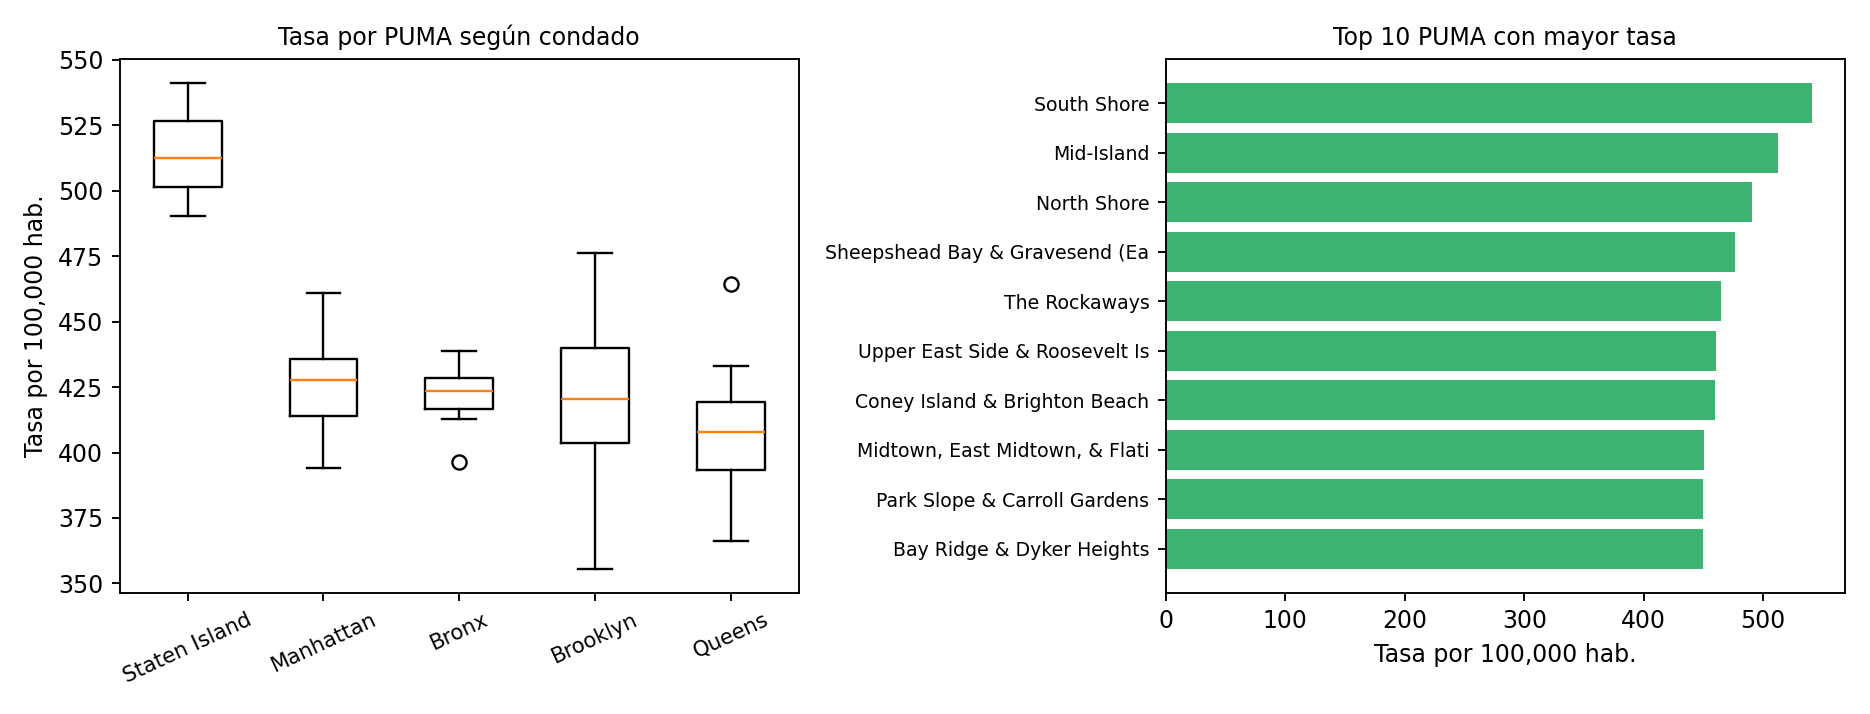
\includegraphics[width=0.92\textwidth]{imagenes/imaged.png}
    \caption{Distribución de la tasa de incidencia de cáncer por PUMA según condado (izquierda) y top 10 de PUMA con mayor tasa (derecha).}
    \label{fig:bono_cancer_puma}
\end{figure}

\subsection{Cruce Multidimensional: Cáncer, Pobreza, Arrestos y Colisiones por Condado}
\label{subsec:bono_cruce}

La Tabla \ref{tab:cruce_condado_cancer} y la Figura \ref{fig:bono_cruce_cancer} integran la tasa promedio de incidencia de cáncer por condado con la proporción de pobreza y las tasas estandarizadas de arrestos y colisiones por cada $100,000$ habitantes calculadas en la Sección \ref{sec:limpieza_transformacion} (Tabla \ref{tab:tasas_100k}). Se observa un contraste demográfico revelador: Staten Island exhibe el mayor promedio de incidencia de cáncer ($514.7$ por $100,000$ hab., asociado a una estructura poblacional de mayor edad media y mayor detección diagnóstica) pero simultáneamente presenta la menor tasa de arrestos ($1,101.2$), la menor tasa de colisiones viales ($666.4$) y una de las menores tasas de pobreza ($13.8\%$). Por el contrario, el Bronx registra la mayor pobreza ($25.8\%$) y la mayor tasa de arrestos ($2,354.5$), mientras que Brooklyn lidera la tasa de siniestralidad vial ($1,051.4$), manteniendo ambos tasas promedio de cáncer cercanas a la media urbana ($421.7$ y $421.1$, respectivamente).

\begin{table}[H]
\centering
\scriptsize
\renewcommand{\arraystretch}{1.2}
\caption{Cruce por condado entre tasa promedio de cáncer (PUMA), pobreza y tasas de arrestos y colisiones por 100,000 habitantes.}
\label{tab:cruce_condado_cancer}
\begin{tabularx}{\linewidth}{l c >{\centering\arraybackslash}X >{\centering\arraybackslash}X >{\centering\arraybackslash}X >{\centering\arraybackslash}X}
\toprule
\textbf{Condado} & \textbf{N.$^{\circ}$ PUMA} & \textbf{Tasa cáncer (prom.)} & \textbf{Pobreza (\%)} & \textbf{Arrestos / 100k} & \textbf{Colisiones / 100k} \\
\midrule
Staten Island & 3 & 514.7 & 13.8 & 1,101.2 & 666.4 \\
Manhattan & 10 & 427.1 & 13.8 & 2,064.1 & 931.9 \\
Bronx & 10 & 421.7 & 25.8 & 2,354.5 & 885.5 \\
Brooklyn & 18 & 421.1 & 18.3 & 1,687.6 & 1,051.4 \\
Queens & 14 & 405.9 & 15.8 & 1,290.8 & 970.3 \\
\bottomrule
\end{tabularx}
\end{table}

\begin{figure}[H]
    \centering
    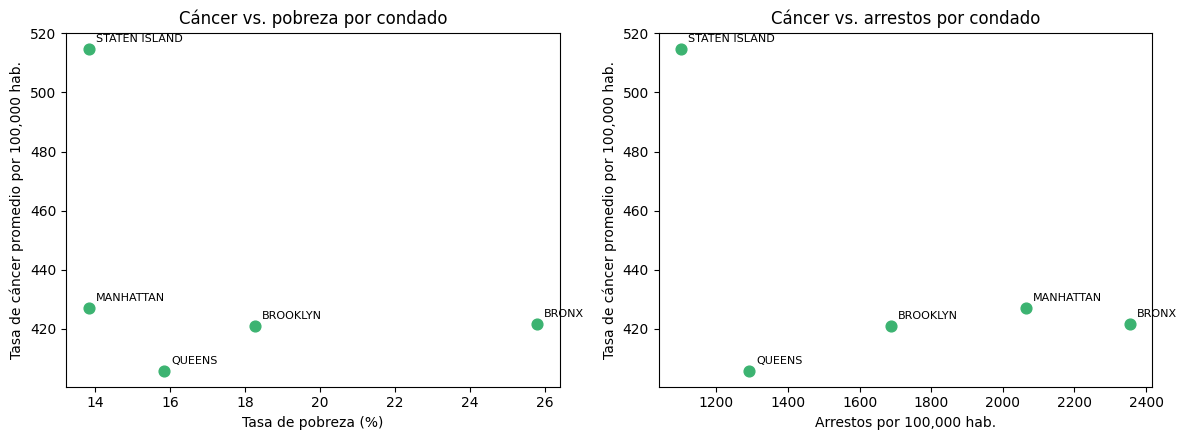
\includegraphics[width=0.9\textwidth]{imagenes/imagee.png}
    \caption{Tasa promedio de cáncer por condado frente a la tasa de pobreza (izquierda) y a los arrestos por 100,000 habitantes (derecha).}
    \label{fig:bono_cruce_cancer}
\end{figure}

\subsection{API Climática: Extracción y Caracterización Meteorológica Diaria en NYC}
\label{subsec:bono_api_clima}

El pipeline consulta las variables meteorológicas diarias para el centro geográfico de la Ciudad de Nueva York ($\text{lat } 40.7128, \text{lon } -74.0060$) cubriendo exactamente las $546$ fechas comprendidas entre el 1 de enero de 2025 (año completo de referencia de colisiones) y el 30 de junio de 2026 (horizonte del conjunto de arrestos y conjunto de prueba de los modelos). El conector soporta el endpoint \texttt{day\_summary} de \textit{OpenWeather One Call API 3.0} \cite{openweather_onecall_2026} y el archivo histórico de \textit{Open-Meteo} \cite{openmeteo_historical_2026}, persistiendo las $546$ observaciones diarias en \texttt{clima\_nyc\_diario.csv} con temperatura mínima y máxima ($^\circ\text{C}$), precipitación total ($\text{mm}$) y velocidad máxima del viento ($\text{m/s}$).

La Tabla \ref{tab:clima_mensual_nyc} y la Figura \ref{fig:bono_clima_diario} sintetizan el comportamiento mensual y diario extraído: julio de 2025 presentó la mayor temperatura máxima media diaria ($31.8\,^\circ\text{C}$) y febrero de 2026 la mínima media diaria más baja ($-7.4\,^\circ\text{C}$), mientras que mayo de 2025 fue el mes de mayor precipitación acumulada ($201.1\text{ mm}$ en $16$ días con lluvia $\ge 1\text{ mm}$).

\begin{table}[H]
\centering
\scriptsize
\caption{Resumen mensual del clima extraído en NYC (enero de 2025 a junio de 2026).}
\label{tab:clima_mensual_nyc}
\setlength{\tabcolsep}{4pt}
\begin{tabularx}{\linewidth}{c c >{\centering\arraybackslash}X >{\centering\arraybackslash}X >{\centering\arraybackslash}X c c}
\toprule
\textbf{Mes} & \textbf{Días} & \textbf{T.~mín. ($^{\circ}$C)} & \textbf{T.~máx. ($^{\circ}$C)} & \textbf{Precip. (mm)} & \textbf{Días lluvia} & \textbf{Viento (m/s)} \\
\midrule
2025-01 & 31 & $-5.3$ & $1.3$ & $30.3$ & 6 & $8.3$ \\
2025-02 & 28 & $-3.2$ & $4.1$ & $79.4$ & 11 & $8.0$ \\
2025-03 & 31 & $2.1$ & $12.6$ & $162.5$ & 10 & $8.5$ \\
2025-04 & 30 & $7.3$ & $17.1$ & $73.1$ & 10 & $8.4$ \\
2025-05 & 31 & $12.7$ & $21.1$ & $201.1$ & 16 & $7.1$ \\
2025-06 & 30 & $18.9$ & $28.8$ & $74.9$ & 12 & $5.8$ \\
2025-07 & 31 & $22.4$ & $31.8$ & $111.4$ & 15 & $6.3$ \\
2025-08 & 31 & $18.4$ & $28.5$ & $23.8$ & 6 & $6.3$ \\
2025-09 & 30 & $16.6$ & $25.6$ & $119.5$ & 9 & $5.7$ \\
2025-10 & 31 & $9.7$ & $18.4$ & $110.5$ & 7 & $7.9$ \\
2025-11 & 30 & $3.6$ & $11.2$ & $49.7$ & 9 & $7.8$ \\
2025-12 & 31 & $-3.9$ & $3.3$ & $79.9$ & 8 & $8.5$ \\
2026-01 & 31 & $-6.2$ & $1.1$ & $68.7$ & 6 & $8.3$ \\
2026-02 & 28 & $-7.4$ & $0.7$ & $53.2$ & 6 & $9.2$ \\
2026-03 & 31 & $2.2$ & $12.3$ & $106.9$ & 12 & $9.2$ \\
2026-04 & 30 & $7.6$ & $18.1$ & $72.7$ & 13 & $6.5$ \\
2026-05 & 31 & $12.9$ & $23.1$ & $98.2$ & 11 & $7.6$ \\
2026-06 & 30 & $18.9$ & $29.0$ & $95.0$ & 14 & $8.7$ \\
\bottomrule
\end{tabularx}
\end{table}

\begin{figure}[H]
    \centering
    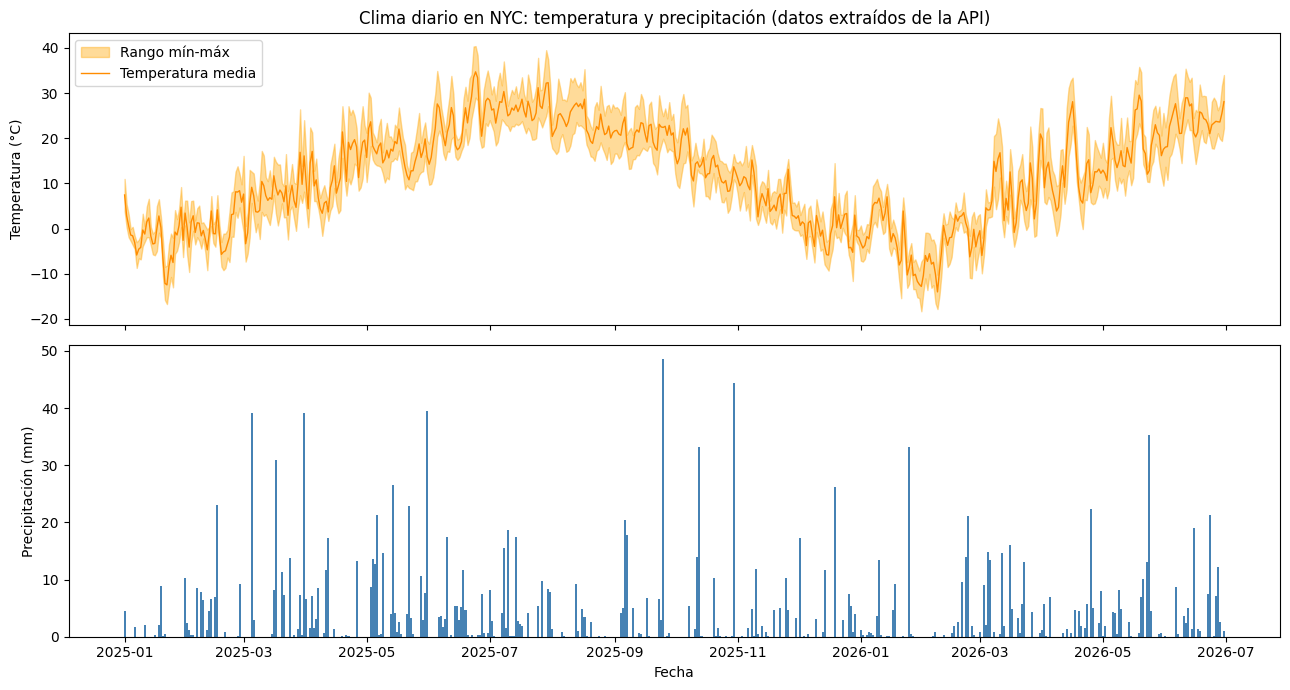
\includegraphics[width=0.88\textwidth]{imagenes/imagef.png}
    \caption{Temperatura (banda mínima--máxima y media diaria) y precipitación diaria en NYC (enero de 2025 a junio de 2026).}
    \label{fig:bono_clima_diario}
\end{figure}

\subsection{Cruce Distribuido en Spark: Clima frente a Colisiones y Arrestos Diarios}
\label{subsec:bono_cruce_clima}

Para conectar las variables meteorológicas con los indicadores de negocio (Objetivo 3), la serie climática se convirtió a un DataFrame distribuido de Spark (\texttt{clima\_sdf}) definiendo la temperatura media diaria $\texttt{temp\_media\_c} = (\texttt{temp\_min\_c} + \texttt{temp\_max\_c})/2$ y el indicador binario de día lluvioso ($\texttt{lluvia} = \mathbb{I}(\texttt{precip\_mm} \ge 1)$). Posteriormente, se efectuó un \texttt{inner join} por fecha con las colisiones diarias agregadas de 2025 ($365$ días) y con los arrestos diarios del primer semestre de 2026 ($181$ días). La Tabla \ref{tab:correlacion_clima} y la Figura \ref{fig:clima_vs_colisiones_arrestos} presentan las correlaciones de Pearson obtenidas.

\begin{table}[H]
\centering
\small
\renewcommand{\arraystretch}{1.2}
\caption{Correlación de Pearson entre variables meteorológicas diarias y el volumen de colisiones, heridos y arrestos.}
\label{tab:correlacion_clima}
\begin{tabular}{l c r r r}
\toprule
\textbf{Indicador Diario} & \textbf{Días ($n$)} & \textbf{Temp.~media ($^{\circ}$C)} & \textbf{Precipitación (mm)} & \textbf{Viento máx. (m/s)} \\
\midrule
Colisiones diarias (2025) & 365 & $+0.301$ & $+0.077$ & $-0.132$ \\
Personas heridas por día (2025) & 365 & $\mathbf{+0.469}$ & $+0.051$ & $-0.159$ \\
Arrestos diarios (2026-I) & 181 & $+0.134$ & $\mathbf{-0.306}$ & $-0.190$ \\
\bottomrule
\end{tabular}
\end{table}

\begin{figure}[H]
    \centering
    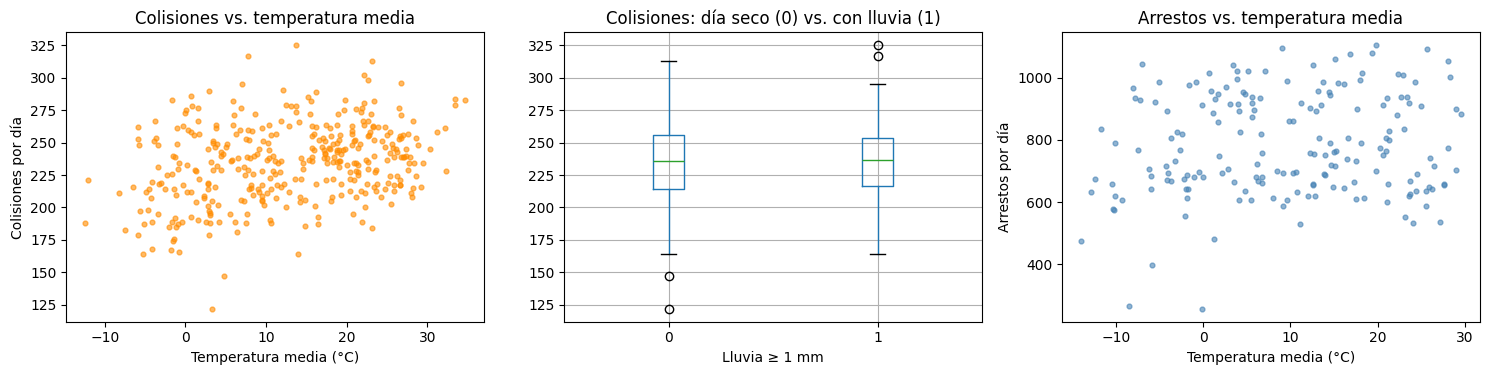
\includegraphics[width=0.95\textwidth]{imagenes/fig_cell_92_1.png}
    \caption{Relación diaria entre temperatura media, condición de lluvia ($\ge 1\text{ mm}$) y volumen de colisiones y arrestos en NYC.}
    \label{fig:clima_vs_colisiones_arrestos}
\end{figure}

\noindent \textbf{Interpretación de negocio:} En 2025, la temperatura media diaria presentó una correlación positiva de $r = +0.301$ con el conteo de colisiones y de $r = +0.469$ con el total diario de personas heridas, explicada por el incremento estacional de flujos peatonales, ciclistas y motociclistas durante la primavera y el verano. El promedio diario en los $119$ días con lluvia fue de $235.1$ colisiones frente a $234.0$ en los $246$ días secos. Por su parte, en el primer semestre de 2026, los arrestos diarios exhibieron una correlación negativa moderada con la precipitación ($r = -0.306$), evidenciando que los eventos de lluvia reducen la actividad en espacio público y las detenciones en vía abierta.


\section{Respuestas a las Preguntas de Negocio Planteadas}
\label{sec:respuestas_preguntas}

En esta sección se presentan las tablas y visualizaciones generadas sobre el clúster de \textbf{Apache Spark} que dan respuesta cuantitativa a las preguntas de negocio formuladas en la Sección \ref{sec:preguntas_negocio}. Para garantizar la comparabilidad temporal entre criminalidad y accidentalidad, el análisis transversal se acota al primer semestre de 2026 (\texttt{2026-01-01} a \texttt{2026-06-30}), y cada hallazgo establece explícitamente su \textbf{punto de contacto con el entendimiento de negocio} descrito en la Sección \ref{sec:entendimiento_negocio}. (La Pregunta 8, por constituir el núcleo del modelado predictivo supervisado, se desarrolla y evalúa integralmente en la Sección \ref{sec:modelado_evaluacion}).

\subsection{Pregunta 1: Concentración Espacial y Temporal de Arrestos por Delitos Graves (Felonías) en los Condados de Nueva York}
\label{subsec:respuesta_q1}

\paragraph{Metodología y alcance:} Como se documentó en la valoración de restricciones (Sección \ref{sec:entendimiento_negocio}), el atributo \texttt{ARREST\_DATE} del conjunto \textit{NYPD Arrest Data} se publica con granularidad diaria (\texttt{MM/dd/yyyy}) sin marca de hora. En consecuencia, se analizó la distribución de los $55,651$ arrestos por delitos graves (\texttt{gravedad\_reportada = 'F'}, felonías) registrados entre enero y junio de 2026 a lo largo de los siete días de la semana y los cinco condados, calculando tanto el volumen absoluto como el peso porcentual intrasemanal dentro de cada condado (Tablas \ref{tab:q1_felonias_dia} y \ref{tab:q1_resumen_boro}, y Figura \ref{fig:q1_felonias_dia_boro}).

\begin{table}[H]
\centering
\scriptsize
\renewcommand{\arraystretch}{1.2}
\caption{Distribución de arrestos por delitos graves (Felonías, \texttt{F}) por día de la semana y condado (conteo y \% intrasemanal, 2026-I).}
\label{tab:q1_felonias_dia}
\begin{tabularx}{\linewidth}{l >{\raggedleft\arraybackslash}X >{\raggedleft\arraybackslash}X >{\raggedleft\arraybackslash}X >{\raggedleft\arraybackslash}X >{\raggedleft\arraybackslash}X >{\raggedleft\arraybackslash}X}
\toprule
\textbf{Día} & \textbf{BRONX} & \textbf{BROOKLYN} & \textbf{MANHATTAN} & \textbf{QUEENS} & \textbf{STATEN ISL.} & \textbf{TOTAL NYC} \\
\midrule
Lunes & 1,528 (11.81\%) & 2,132 (12.47\%) & 1,282 (10.59\%) & 1,401 (12.21\%) & 253 (12.44\%) & 6,596 (11.85\%) \\
Martes & \textbf{2,440 (18.85\%)} & 3,024 (17.69\%) & 2,059 (17.01\%) & 2,004 (17.47\%) & 354 (17.41\%) & 9,881 (17.76\%) \\
Miércoles & 2,431 (18.78\%) & \textbf{3,101 (18.14\%)} & 2,145 (17.72\%) & \textbf{2,161 (18.84\%)} & 352 (17.31\%) & \textbf{10,190 (18.31\%)} \\
Jueves & 2,068 (15.98\%) & 2,861 (16.73\%) & \textbf{2,213 (18.28\%)} & 1,959 (17.07\%) & \textbf{368 (18.10\%)} & 9,469 (17.01\%) \\
Viernes & 1,751 (13.53\%) & 2,414 (14.12\%) & 1,884 (15.56\%) & 1,587 (13.83\%) & 334 (16.43\%) & 7,970 (14.32\%) \\
Sábado & 1,388 (10.72\%) & 1,860 (10.88\%) & 1,377 (11.38\%) & 1,205 (10.50\%) & 183 (9.00\%) & 6,013 (10.80\%) \\
Domingo & 1,337 (10.33\%) & 1,705 (9.97\%) & 1,145 (9.46\%) & 1,156 (10.08\%) & 189 (9.30\%) & 5,532 (9.94\%) \\
\midrule
\textbf{Total} & \textbf{12,943 (100\%)} & \textbf{17,097 (100\%)} & \textbf{12,105 (100\%)} & \textbf{11,473 (100\%)} & \textbf{2,033 (100\%)} & \textbf{55,651 (100\%)} \\
\bottomrule
\end{tabularx}
\end{table}

\begin{table}[H]
\centering
\scriptsize
\renewcommand{\arraystretch}{1.2}
\caption{Indicadores de concentración intrasemanal de felonías por condado.}
\label{tab:q1_resumen_boro}
\resizebox{\textwidth}{!}{%
\begin{tabular}{l r c r r r}
\toprule
\textbf{Condado (\texttt{BORO})} & \textbf{Total felonías} & \textbf{Día pico} & \textbf{Arrestos día pico} & \textbf{Concentración Mar--Jue (\%)} & \textbf{Fin de semana Sáb--Dom (\%)} \\
\midrule
BROOKLYN & 17,097 & Miércoles & 3,101 & 52.56\% & 20.85\% \\
BRONX & 12,943 & Martes & 2,440 & \textbf{53.61\%} & 21.05\% \\
MANHATTAN & 12,105 & Jueves & 2,213 & 53.01\% & 20.84\% \\
QUEENS & 11,473 & Miércoles & 2,161 & 53.38\% & 20.58\% \\
STATEN ISLAND & 2,033 & Jueves & 368 & 52.82\% & 18.30\% \\
\bottomrule
\end{tabular}%
}
\end{table}

\begin{figure}[H]
    \centering
    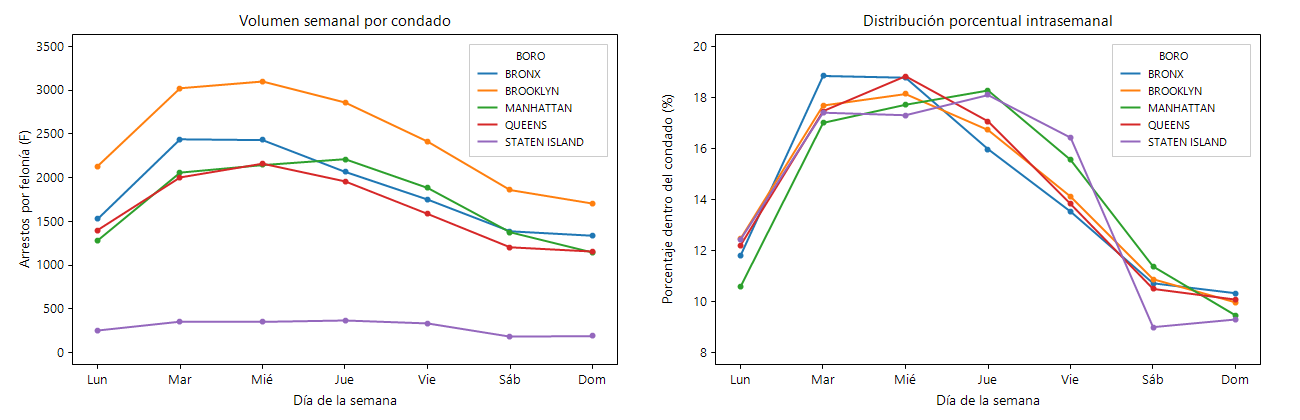
\includegraphics[width=0.96\textwidth]{imagenes/fig_q1_felonias_dia_boro.png}
    \caption{Volumen semanal absoluto (izquierda) y distribución porcentual intrasemanal (derecha) de arrestos por felonías (\texttt{F}) según condado.}
    \label{fig:q1_felonias_dia_boro}
\end{figure}

\paragraph{Interpretación y punto de contacto con el entendimiento de negocio:}
Brooklyn lidera el volumen absoluto de arrestos por delitos graves ($17,097$), seguido por el Bronx ($12,943$) y Manhattan ($12,105$). Sin embargo, al examinar el patrón porcentual intrasemanal (Figura \ref{fig:q1_felonias_dia_boro}, derecha), se descubre una regularidad operativa contundente: en los cinco condados, \textbf{entre el $52.56\%$ y el $53.61\%$ de todos los arrestos por felonías ocurren en tan solo tres días (martes, miércoles y jueves)}, sumando $29,540$ detenciones, mientras que los sábados y domingos apenas concentran el $20.75\%$ ($11,545$). Asimismo, se identifica un desplazamiento territorial del pico máximo: el Bronx alcanza su máximo los martes ($18.85\%$), Brooklyn y Queens los miércoles ($18.14\%$ y $18.84\%$), y Manhattan y Staten Island los jueves ($18.28\%$ y $18.10\%$). En conexión directa con el \textbf{Objetivo de Negocio 1 (\textit{NYPD CompStat})} de la Entrega 1, esta evidencia permite programar de manera escalonada los escuadrones especializados de cumplimiento de órdenes judiciales (\textit{warrant squads}) y refuerzos de patrulla: focalizando el Bronx los martes, Brooklyn y Queens los miércoles, y Manhattan los jueves.

\subsection{Pregunta 2: Correlación entre Pobreza Ponderada y Arrestos por Delitos Menores}
\label{subsec:respuesta_q2}

\paragraph{Metodología:} Se calculó la tasa de pobreza municipal ponderada de cada condado empleando el factor de expansión personal \texttt{PWGTP} sobre los registros válidos de \texttt{NYCgov\_Pov\_Stat} ($\in \{1, 2\}$), y se contrastó mediante el coeficiente de correlación lineal de Pearson ($r$) y su valor-$p$ bilateral frente a: (i) el conteo absoluto de arrestos por delitos menores (\texttt{gravedad\_reportada = 'M'}) en el primer semestre de 2026, y (ii) la tasa de arrestos por delitos menores por cada $100,000$ habitantes (Tabla \ref{tab:q2_pobreza_menores} y Figura \ref{fig:q2_pobreza_menores}).

\begin{table}[H]
\centering
\small
\renewcommand{\arraystretch}{1.2}
\caption{Tasa de pobreza ponderada (\texttt{PWGTP}) y arrestos por delitos menores (\texttt{M}) en volumen absoluto y tasa por 100,000 habitantes.}
\label{tab:q2_pobreza_menores}
\begin{tabular}{l r r r}
\toprule
\textbf{Condado (\texttt{BORO})} & \textbf{Pobreza ponderada (\%)} & \textbf{Arrestos menores (\texttt{M})} & \textbf{Menores por 100,000 hab.} \\
\midrule
BRONX & \textbf{27.12\%} & 19,268 & \textbf{1,388.12} \\
BROOKLYN & 20.31\% & \textbf{24,442} & 962.04 \\
QUEENS & 17.02\% & 16,767 & 744.95 \\
STATEN ISLAND & 16.00\% & 3,115 & 663.62 \\
MANHATTAN & 15.12\% & 19,337 & 1,243.81 \\
\bottomrule
\end{tabular}
\end{table}

\begin{figure}[H]
    \centering
    \begin{minipage}[c]{0.49\textwidth}
        \centering
        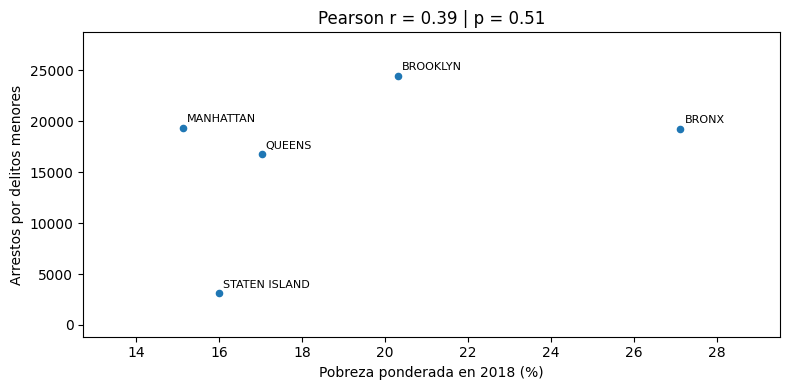
\includegraphics[width=\linewidth]{imagenes/fig_cell_51_1.png}
    \end{minipage}\hfill
    \begin{minipage}[c]{0.49\textwidth}
        \centering
        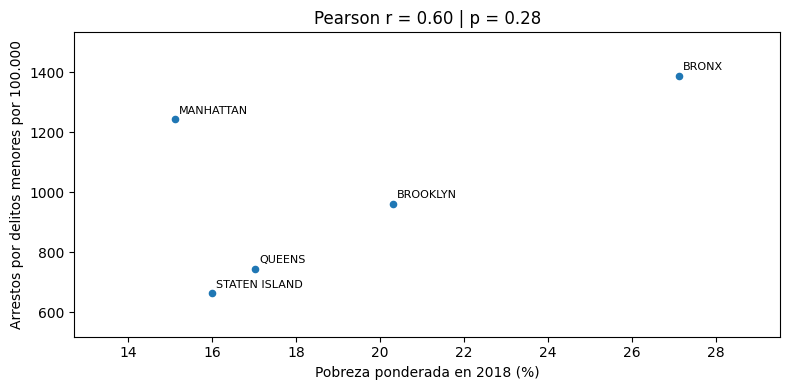
\includegraphics[width=\linewidth]{imagenes/fig_cell_51_2.png}
    \end{minipage}
    \caption{Diagramas de dispersión y correlación de Pearson entre pobreza ponderada (2018) y arrestos por delitos menores en conteo bruto (izquierda, $r=0.39$) y por 100,000 habitantes (derecha, $r=0.60$).}
    \label{fig:q2_pobreza_menores}
\end{figure}

\paragraph{Interpretación y punto de contacto con el entendimiento de negocio:}
Al comparar la pobreza ponderada con el conteo bruto de arrestos menores se obtiene una correlación débil de $r = 0.39$ ($p = 0.51$), debido a que Brooklyn domina por tamaño poblacional ($24,442$ casos) y Manhattan registra $19,337$ casos pese a tener la menor tasa de pobreza residente ($15.12\%$). Al corregir por población mediante la tasa por $100,000$ habitantes, la asociación positiva asciende a $r = 0.60$ ($p = 0.28$), ubicando al Bronx en el primer lugar tanto en pobreza ponderada ($27.12\%$) como en tasa de delitos menores ($1,388.12$ por $100,000$ hab.). Aunque con $n = 5$ condados el valor-$p$ no alcanza significancia estadística al $5\%$, el comportamiento confirma el diagnóstico macroeconómico planteado en la Sección \ref{sec:entendimiento_negocio} (\textbf{Objetivos 1 y 3}): en el Bronx la alta incidencia per cápita de contravenciones y delitos menores coincide con la vulnerabilidad económica estructural, mientras que en Manhattan ($1,243.81$ por $100,000$ hab. residentes) la tasa está inflada por el flujo diario de población flotante comercial y turística en el sistema de transporte y zonas comerciales.

\subsection{Pregunta 3: Factores Contribuyentes y Tipos de Vehículos en Colisiones con Peatones o Ciclistas Afectados}
\label{subsec:respuesta_q3}

\paragraph{Metodología:} Se filtraron las colisiones del primer semestre de 2026 con al menos un peatón o ciclista herido o fallecido. Para evitar subestimar causas o vehículos reportados en las posiciones secundarias, se inspeccionaron las cinco columnas de cada familia (\texttt{CONTRIBUTING FACTOR VEHICLE 1--5} y \texttt{VEHICLE TYPE CODE 1--5}), aplicando \texttt{array\_distinct} por \texttt{COLLISION\_ID} para contar una sola vez cada categoría presente en el siniestro y excluyendo valores genéricos (\texttt{UNSPECIFIED}, \texttt{UNKNOWN}, \texttt{DOES NOT APPLY} y \texttt{SIN\_VEHICULO\_*}) (Tabla \ref{tab:q3_vulnerables} y Figura \ref{fig:q3_vulnerables}).

\begin{table}[H]
\centering
\scriptsize
\renewcommand{\arraystretch}{1.2}
\caption{Top 10 de factores contribuyentes y tipos de vehículo en colisiones con peatones o ciclistas heridos/fallecidos (2026-I).}
\label{tab:q3_vulnerables}
\begin{tabularx}{\linewidth}{c X r c X r}
\toprule
\textbf{\#} & \textbf{Factor Contribuyente Reportado} & \textbf{Colisiones} & \textbf{\#} & \textbf{Tipo de Vehículo Reportado} & \textbf{Colisiones} \\
\midrule
1 & DRIVER INATTENTION/DISTRACTION & \textbf{1,686} & 1 & STATION WAGON/SPORT UTILITY VEHICLE & \textbf{1,741} \\
2 & FAILURE TO YIELD RIGHT-OF-WAY & \textbf{1,243} & 2 & SEDAN & \textbf{1,554} \\
3 & PEDESTRIAN/BICYCLIST ERROR/CONFUSION & 378 & 3 & BICYCLIST & 1,035 \\
4 & TRAFFIC CONTROL DISREGARDED & 170 & 4 & BIKE & 982 \\
5 & BACKING UNSAFELY & 144 & 5 & 4 DR SEDAN & 762 \\
6 & UNSAFE SPEED & 140 & 6 & TAXI & 242 \\
7 & PASSING OR LANE USAGE IMPROPER & 135 & 7 & PICK-UP TRUCK & 162 \\
8 & TURNING IMPROPERLY & 115 & 8 & VAN & 106 \\
9 & VIEW OBSTRUCTED/LIMITED & 99 & 9 & BUS & 83 \\
10 & OTHER VEHICULAR & 98 & 10 & MOPED & 74 \\
\bottomrule
\end{tabularx}
\end{table}

\begin{figure}[H]
    \centering
    \begin{minipage}[c]{0.49\textwidth}
        \centering
        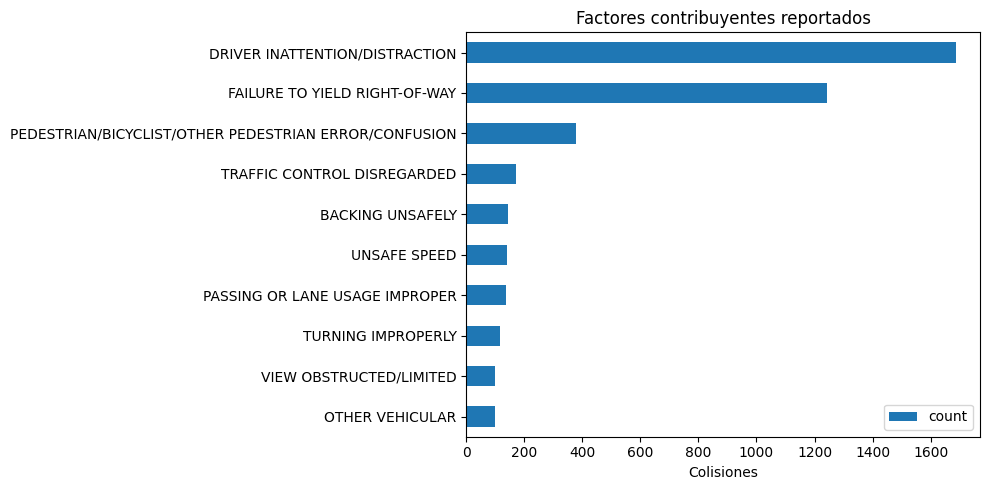
\includegraphics[width=\linewidth]{imagenes/fig_cell_54_1.png}
    \end{minipage}\hfill
    \begin{minipage}[c]{0.49\textwidth}
        \centering
        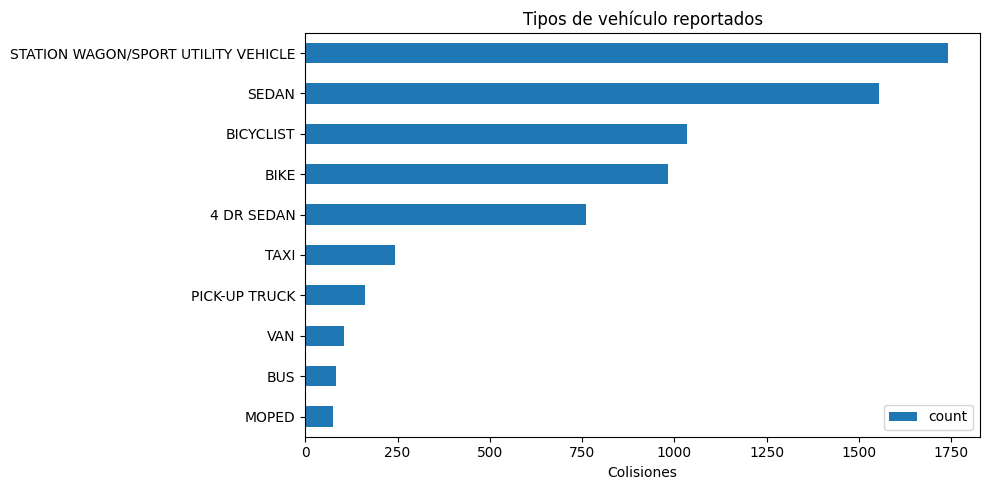
\includegraphics[width=\linewidth]{imagenes/fig_cell_54_2.png}
    \end{minipage}
    \caption{Principales factores contribuyentes (izquierda) y tipos de vehículo (derecha) en siniestros con afectación de peatones o ciclistas.}
    \label{fig:q3_vulnerables}
\end{figure}

\paragraph{Interpretación y punto de contacto con el entendimiento de negocio:}
Dos factores humanos del conductor concentran por amplio margen la accidentalidad contra actores viales vulnerables: la \textbf{distracción o falta de atención del conductor (\texttt{DRIVER INATTENTION/DISTRACTION}, $1,686$ colisiones)} y el \textbf{no ceder la prelación de paso (\texttt{FAILURE TO YIELD RIGHT-OF-WAY}, $1,243$ colisiones)}, seguidos a gran distancia por error/confusión del peatón o ciclista ($378$), desacato de señales de tránsito ($170$), reversa insegura ($144$) y velocidad insegura ($140$). En cuanto al parque automotor, las \textbf{camionetas familiares y SUV (\texttt{STATION WAGON/SPORT UTILITY VEHICLE}, $1,741$ colisiones)} encabezan los siniestros con vulnerables, superando incluso a los sedanes ($1,554$). Esto se conecta directamente con el \textbf{Objetivo de Negocio 2 (\textit{NYC DOT Vision Zero})} de la Entrega 1: la mayor altura del capó y los puntos ciegos de las SUV incrementan la severidad de los atropellamientos en giros, por lo que el NYC DOT debe priorizar fases semafóricas exclusivas para peatones (\textit{Leading Pedestrian Intervals}, LPI) e isletas de refugio en intersecciones para mitigar directamente el factor \texttt{FAILURE TO YIELD RIGHT-OF-WAY}.

\subsection{Pregunta 4: Desempleo, Nivel Educativo y Siniestralidad Vial Fatal por Condado}
\label{subsec:respuesta_q4}

\paragraph{Metodología:} Se estimó la tasa ponderada de desempleo en la fuerza laboral civil ($\texttt{ESR} = 3$ sobre $\texttt{ESR} \in \{1, 2, 3\}$) y la distribución porcentual del nivel educativo alcanzado en adultos de $25$ años o más ($\texttt{SCHL} \in [1, 24]$) usando \texttt{PWGTP}. Estos indicadores se cruzaron con el conteo y la tasa de colisiones fatales (al menos un fallecido) por cada $100,000$ habitantes en el primer semestre de 2026 (Tabla \ref{tab:q4_desempleo_edu_fatal} y Figura \ref{fig:q4_desempleo_edu_fatal}).

\begin{table}[H]
\centering
\scriptsize
\renewcommand{\arraystretch}{1.2}
\caption{Indicadores laborales y educativos (ponderados con \texttt{PWGTP}) frente a la tasa de colisiones fatales por 100,000 habitantes (2026-I).}
\label{tab:q4_desempleo_edu_fatal}
\resizebox{\textwidth}{!}{%
\begin{tabular}{l r r r r r r r}
\toprule
\textbf{Condado} & \textbf{Desempleo (\%)} & \textbf{Sin sec. (\%)} & \textbf{Secundaria (\%)} & \textbf{Sup. sin grado (\%)} & \textbf{Univ. o sup. (\%)} & \textbf{Fatales} & \textbf{Fatales / 100k} \\
\midrule
QUEENS & 5.11\% & 17.32\% & 26.53\% & 22.29\% & 33.87\% & \textbf{31} & \textbf{1.38} \\
BRONX & \textbf{9.56\%} & \textbf{26.26\%} & 27.34\% & 25.15\% & 21.25\% & 19 & 1.37 \\
MANHATTAN & 4.36\% & 11.80\% & 12.43\% & 13.35\% & \textbf{62.41\%} & 21 & 1.35 \\
BROOKLYN & 4.67\% & 16.42\% & 24.94\% & 19.09\% & 39.55\% & 26 & 1.02 \\
STATEN ISLAND & 4.40\% & 12.17\% & \textbf{30.91\%} & 23.61\% & 33.31\% & 3 & 0.64 \\
\bottomrule
\end{tabular}%
}
\end{table}

\begin{figure}[H]
    \centering
    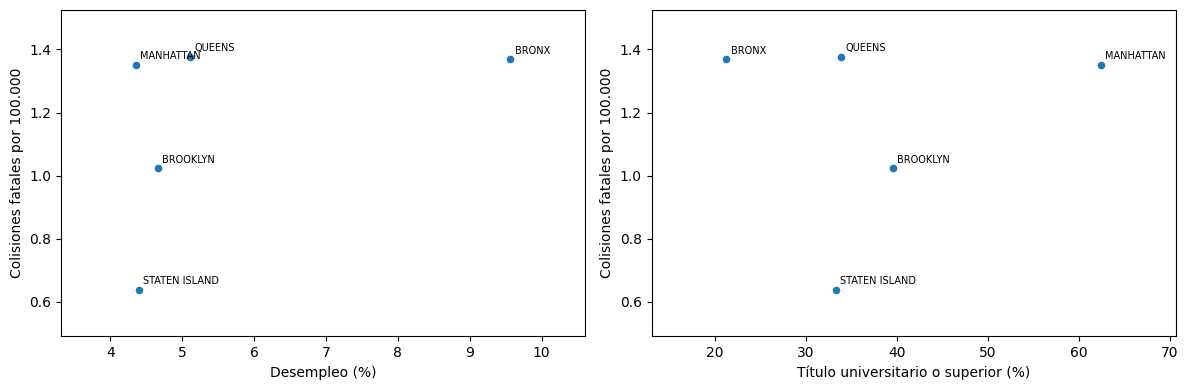
\includegraphics[width=0.95\textwidth]{imagenes/fig_cell_57_1.png}
    \caption{Tasa de colisiones fatales por 100,000 habitantes frente a la tasa de desempleo (izquierda) y al porcentaje de población con título universitario o superior (derecha).}
    \label{fig:q4_desempleo_edu_fatal}
\end{figure}

\paragraph{Interpretación y punto de contacto con el entendimiento de negocio:}
Los resultados revelan que la mortalidad vial por cada $100,000$ habitantes es prácticamente idéntica en tres condados con perfiles socioeconómicos opuestos: \textbf{Queens ($1.38$), el Bronx ($1.37$) y Manhattan ($1.35$)}, pese a que el Bronx duplica la tasa de desempleo de Manhattan ($9.56\%$ frente a $4.36\%$) y Manhattan casi triplica la proporción de graduados universitarios del Bronx ($62.41\%$ frente a $21.25\%$). Esto responde directamente a la hipótesis planteada en los \textbf{Objetivos 2 y 3} del entendimiento de negocio: a escala agregada de condado, la letalidad vial no está determinada de forma lineal simple por el nivel educativo o el desempleo promedio del condado, sino por la combinación de déficit de infraestructura segura en corredores de carga (como en el Bronx y Queens) y la altísima densidad de interacciones peatonales en centros comerciales (Manhattan), lo que exige descender a una escala microterritorial de cuadrículas como se realiza en la Pregunta 5 y en el modelo K-Means.

\subsection{Pregunta 5: Las Cinco ``Zonas Calientes Duales'' (\textit{Hotspots}) de Arrestos y Colisiones Fatales}
\label{subsec:respuesta_q5}

\paragraph{Metodología:} Se discretizaron los registros con coordenadas válidas del primer semestre de 2026 en celdas uniformes de $0.01^\circ \times 0.01^\circ$ ($\approx 1.1\text{ km} \times 0.85\text{ km}$). Sobre las celdas que registraron simultáneamente arrestos y colisiones fatales, se construyó un índice compuesto promediando el rango percentil (\texttt{percent\_rank}) del volumen de arrestos y el rango percentil de colisiones fatales:
\[
\text{Índice}_{x,y} = \frac{1}{2}\Big[\text{PercentRank}(\text{arrestos}_{x,y}) + \text{PercentRank}(\text{fatales}_{x,y})\Big].
\]
La Tabla \ref{tab:q5_hotspots} y la Figura \ref{fig:q5_hotspots} presentan las cinco cuadrículas críticas que encabezan el ranking de la ciudad.

\begin{table}[H]
\centering
\scriptsize
\renewcommand{\arraystretch}{1.2}
\caption{Top 5 de cuadrículas urbanas ($0.01^\circ \times 0.01^\circ$) con mayor concentración conjunta de arrestos y colisiones fatales (2026-I).}
\label{tab:q5_hotspots}
\resizebox{\textwidth}{!}{%
\begin{tabular}{c r r l r r r}
\toprule
\textbf{Puesto} & \textbf{Latitud centro} & \textbf{Longitud centro} & \textbf{Sector urbano de referencia} & \textbf{Arrestos} & \textbf{Colisiones fatales} & \textbf{Índice conjunto} \\
\midrule
1 & $40.845^\circ$ & $-73.905^\circ$ & Bronx Central (\textit{Tremont / Cross Bronx Expwy}) & \textbf{1,584} & \textbf{2} & \textbf{0.9674} \\
2 & $40.675^\circ$ & $-73.905^\circ$ & Brooklyn Este (\textit{Brownsville / Broadway Jct}) & \textbf{1,107} & \textbf{2} & \textbf{0.9511} \\
3 & $40.755^\circ$ & $-73.965^\circ$ & Manhattan Midtown East (\textit{2nd/3rd Ave \& E 50s}) & 138 & \textbf{2} & 0.7554 \\
4 & $40.635^\circ$ & $-74.135^\circ$ & Staten Island North Shore (\textit{Port Richmond}) & 109 & \textbf{2} & 0.7228 \\
5 & $40.715^\circ$ & $-73.975^\circ$ & Manhattan Lower East Side (\textit{Williamsburg Br / FDR}) & 77 & \textbf{2} & 0.6902 \\
\bottomrule
\end{tabular}%
}
\end{table}

\begin{figure}[H]
    \centering
    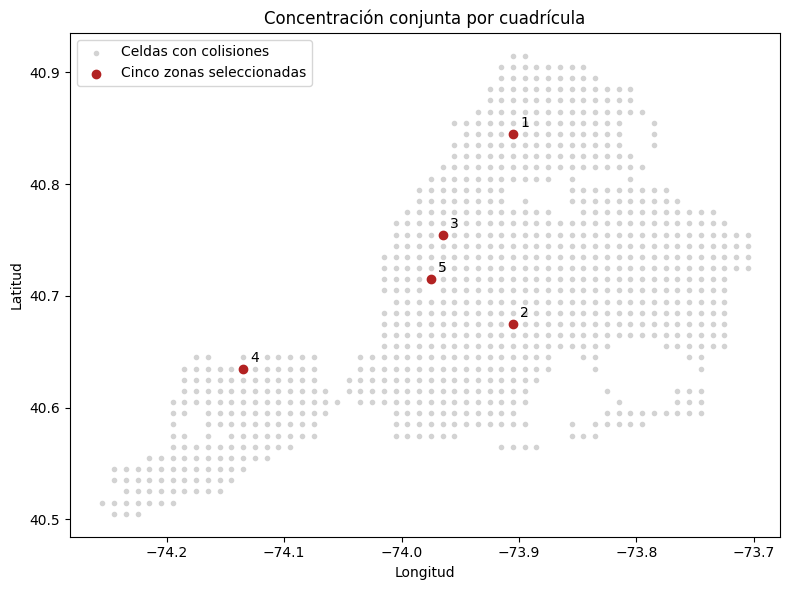
\includegraphics[width=0.72\textwidth]{imagenes/fig_cell_60_1.png}
    \caption{Mapa de cuadrículas activas con colisiones en NYC y localización exacta de las 5 zonas calientes duales seleccionadas.}
    \label{fig:q5_hotspots}
\end{figure}

\paragraph{Interpretación y punto de contacto con el entendimiento de negocio:}
Las dos primeras zonas calientes duales sobresalen de manera extraordinaria: la cuadrícula centrada en $(40.845^\circ, -73.905^\circ)$ en el corredor central del Bronx (\textit{Tremont / Cross Bronx Expressway}, área de los precintos 44, 46 y 48) acumula \textbf{$1,584$ arrestos y $2$ colisiones mortales} ($\text{índice} = 0.9674$), seguida por la cuadrícula $(40.675^\circ, -73.905^\circ)$ en el este de Brooklyn (\textit{Brownsville / Broadway Junction}, área de los precintos 73 y 75, que encabezaban el Elemento 7 del EDA) con \textbf{$1,107$ arrestos y $2$ colisiones mortales} ($\text{índice} = 0.9511$). Este resultado materializa el criterio de éxito central de la Sección \ref{sec:entendimiento_negocio}: entrega a la Alcaldía de Nueva York cinco coordenadas precisas de menos de $1\text{ km}^2$ donde la inversión simultánea en iluminación peatonal, rediseño de cruces arteriales y presencia policial genera un impacto directo tanto en \textit{CompStat} como en \textit{Vision Zero}.

\subsection{Pregunta 6: Perfil Demográfico de los Arrestos según Nivel de Gravedad de la Ofensa}
\label{subsec:respuesta_q6}

\paragraph{Metodología:} Utilizando funciones de ventana particionadas por la gravedad original reportada (\texttt{V}, \texttt{M}, \texttt{F}), se identificó el perfil demográfico conjunto más frecuente (\texttt{AGE\_GROUP}, \texttt{PERP\_SEX}, \texttt{PERP\_RACE}) y se graficó la composición porcentual separada de cada variable demográfica por categoría de gravedad (Tabla \ref{tab:q6_perfil_demografico} y Figura \ref{fig:q6_perfil_demografico}).

\begin{table}[H]
\centering
\scriptsize
\renewcommand{\arraystretch}{1.2}
\caption{Perfil demográfico conjunto modal según el nivel de gravedad reportado de la ofensa (2026-I).}
\label{tab:q6_perfil_demografico}
\resizebox{\textwidth}{!}{%
\begin{tabular}{c l c c l r}
\toprule
\textbf{Código} & \textbf{Nivel de gravedad} & \textbf{Grupo etario modal} & \textbf{Sexo modal} & \textbf{Raza registrada modal} & \textbf{Arrestos del perfil modal} \\
\midrule
\texttt{F} & Felonía (\textit{Felony}) & \texttt{25-44} & \texttt{M} (Masculino) & \texttt{BLACK} & 12,539 \\
\texttt{M} & Delito menor (\textit{Misdemeanor}) & \texttt{25-44} & \texttt{M} (Masculino) & \texttt{BLACK} & 17,778 \\
\texttt{V} & Contravención (\textit{Violation}) & \texttt{25-44} & \texttt{M} (Masculino) & \texttt{BLACK} & 570 \\
\bottomrule
\end{tabular}%
}
\end{table}

\begin{figure}[H]
    \centering
    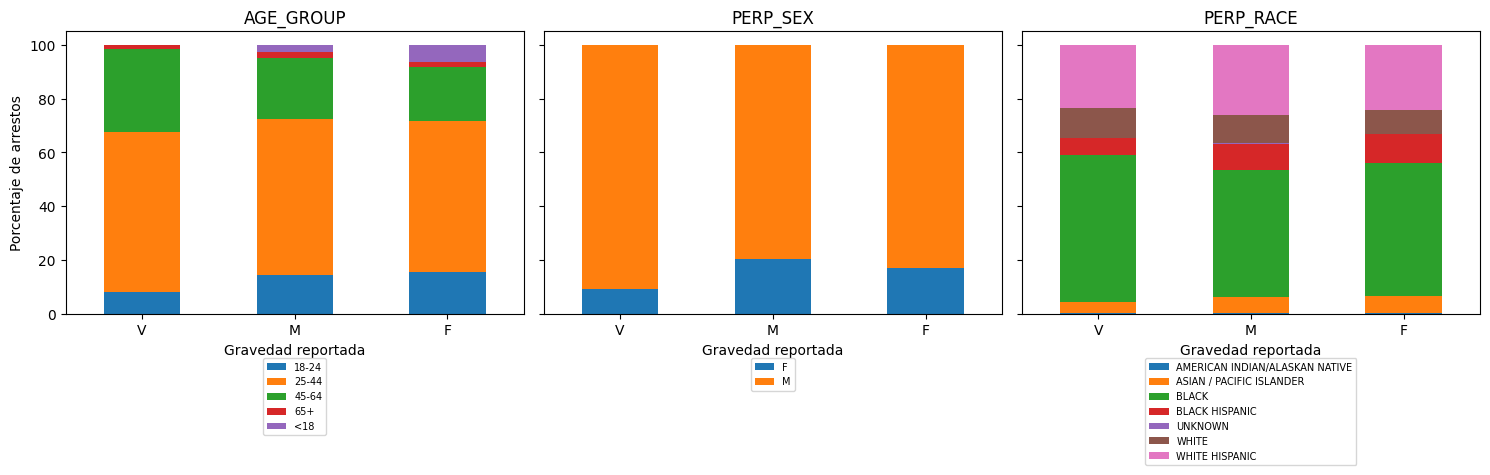
\includegraphics[width=0.98\textwidth]{imagenes/fig_cell_63_1.png}
    \caption{Composición porcentual de los arrestos según gravedad reportada (\texttt{V}, \texttt{M}, \texttt{F}) desagregada por grupo etario, sexo y raza.}
    \label{fig:q6_perfil_demografico}
\end{figure}

\paragraph{Interpretación y punto de contacto con el entendimiento de negocio:}
En las tres categorías penales (\texttt{V}, \texttt{M} y \texttt{F}), el grupo modal invariante corresponde a hombres de $25$ a $44$ años registrados como \texttt{BLACK} ($17,778$ en delitos menores, $12,539$ en felonías y $570$ en contravenciones). Asimismo, la Figura \ref{fig:q6_perfil_demografico} muestra que la proporción de jóvenes de \texttt{18-24} años y menores de $18$ años (\texttt{<18}) es mayor en las felonías (\texttt{F}) que en los delitos menores (\texttt{M}). En línea con los \textbf{Objetivos 1 y 3} del entendimiento de negocio, es fundamental subrayar que estas cifras reflejan la composición de las detenciones policiales registradas y deben articularse con programas de inserción laboral juvenil y prevención social comunitaria de \textit{NYC Opportunity} en los distritos de mayor vulnerabilidad.

\subsection{Pregunta 7: Comportamiento Horario de las Colisiones en Manhattan frente a Staten Island}
\label{subsec:respuesta_q7}

\paragraph{Metodología:} Se compararon las colisiones con hora válida del primer semestre de 2026 entre Manhattan (condado de altísima densidad comercial y población flotante) y Staten Island (condado residencial y suburbano), analizando tanto la frecuencia horaria absoluta como la curva porcentual normalizada dentro de cada condado para aislar la forma del patrón intradiario respecto del tamaño total (Tabla \ref{tab:q7_horario_manhattan_si} y Figura \ref{fig:q7_horario_manhattan_si}).

\begin{table}[H]
\centering
\scriptsize
\renewcommand{\arraystretch}{1.2}
\caption{Resumen comparativo del régimen horario de colisiones entre Manhattan y Staten Island (2026-I).}
\label{tab:q7_horario_manhattan_si}
\resizebox{\textwidth}{!}{%
\begin{tabular}{l r c r r}
\toprule
\textbf{Condado (\texttt{BOROUGH})} & \textbf{Total colisiones (2026-I)} & \textbf{Hora pico} & \textbf{Colisiones en hora pico} & \textbf{\% en hora pico dentro del condado} \\
\midrule
MANHATTAN & \textbf{7,347} & \textbf{16:00 h} & \textbf{507} & 6.90\% \\
STATEN ISLAND & 1,570 & \textbf{15:00 h} & 112 & \textbf{7.13\%} \\
\bottomrule
\end{tabular}%
}
\end{table}

\begin{figure}[H]
    \centering
    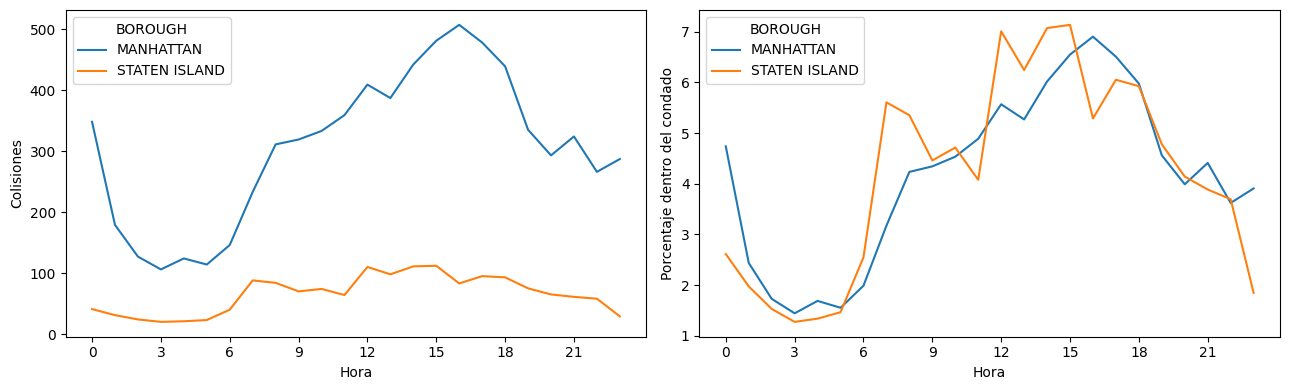
\includegraphics[width=0.96\textwidth]{imagenes/fig_cell_66_1.png}
    \caption{Comparación del volumen horario absoluto (izquierda) y del porcentaje intradiario dentro de cada condado (derecha) de las colisiones en Manhattan y Staten Island.}
    \label{fig:q7_horario_manhattan_si}
\end{figure}

\paragraph{Interpretación y punto de contacto con el entendimiento de negocio:}
Manhattan registra un volumen $4.68$ veces superior al de Staten Island ($7,347$ frente a $1,570$ colisiones). Sin embargo, la gráfica de proporciones internas (Figura \ref{fig:q7_horario_manhattan_si}, derecha) revela dos dinámicas urbanas estructuralmente distintas que validan la hipótesis del \textit{``Efecto Manhattan''} formulada en el entendimiento de negocio (\textbf{Objetivo 2 --- NYC DOT}):
\begin{enumerate}
    \item \textbf{En Staten Island (patrón bimodal pendular escolar--laboral):} Se observan dos picos agudos en horas de desplazamiento residencial: un pico matutino entre las \textbf{07:00 y las 08:00 h} ($\sim 5.6\%$ por hora) y un pico vespertino temprano entre las \textbf{12:00 y las 15:00 h} (máximo a las \textbf{15:00 h} con $112$ choques, $7.13\%$, coincidente con la salida escolar y laboral suburbana), cayendo abruptamente en la noche y la madrugada ($<2\%$ a las 23:00--05:00 h).
    \item \textbf{En Manhattan (meseta comercial continua y actividad nocturna):} El ascenso matutino es más gradual, sostiene una meseta alta durante toda la jornada laboral y comercial con máximo a las \textbf{16:00 h} ($507$ colisiones, $6.90\%$), y mantiene una proporción significativamente superior durante la noche y la madrugada (\textbf{21:00 a 01:00 h}, con casi el $4.8\%$ a las 00:00 h frente al $2.6\%$ en Staten Island), impulsada por la vida nocturna, taxis y logística urbana. Esto justifica planes de semaforización adaptativa y control nocturno diferenciados por condado.
\end{enumerate}


\section{Modelado y Evaluación de Aprendizaje de Máquina en Spark MLlib}
\label{sec:modelado_evaluacion}

Esta sección desarrolla de forma estructurada los numerales 3, 4, 5 y 6 de la entrega final sobre el clúster de \textbf{Apache Spark} (\texttt{spark://10.195.34.34:7077}) empleando la biblioteca distribuida \textbf{Spark MLlib} (\texttt{pyspark.ml}) \cite{meng2016mllib}, y da respuesta cuantitativa a la \textbf{Pregunta de Negocio 8} sobre las variables asociadas con la fatalidad vial.

\subsection{Selección y Justificación de Técnicas de Aprendizaje de Máquina}
\label{subsec:seleccion_tecnicas_num3}

En correspondencia directa con los objetivos de negocio establecidos en la Sección \ref{sec:entendimiento_negocio}, se seleccionaron una técnica de aprendizaje supervisado y una técnica de aprendizaje no supervisado nativas de \textbf{Spark MLlib}:

\begin{enumerate}
    \item \textbf{Técnica Supervisada --- Regresión Logística Regularizada (\texttt{LogisticRegression}):}
    \begin{itemize}
        \item \textit{Objetivo de negocio asociado (Objetivo 2 --- Vision Zero y Pregunta 8):} Estimar la probabilidad de que una colisión vehicular reportada resulte en al menos una persona fallecida ($\texttt{label} = \mathbb{I}(\texttt{NUMBER OF PERSONS KILLED} > 0) \in \{0, 1\}$) e identificar qué familias de variables (hora, ubicación, tipo de vehículo y factor contribuyente) presentan mayor asociación con un desenlace fatal.
        \item \textit{Justificación técnica y de negocio:} El histórico de colisiones provee una etiqueta binaria verificada para cada siniestro. A diferencia de modelos de caja negra, la Regresión Logística en MLlib permite: (i) incorporar pesos por observación (\texttt{weightCol}) para compensar el desbalance extremo de la clase fatal ($\approx 0.25\%$), (ii) controlar el sobreajuste sobre cientos de categorías codificadas mediante regularización L2 (\texttt{regParam}), y (iii) inspeccionar directamente el signo y la magnitud de los coeficientes ajustados ($\beta_j$), ofreciendo interpretabilidad auditable para las autoridades de transporte y emergencias de Nueva York.
    \end{itemize}

    \item \textbf{Técnica No Supervisada --- Agrupamiento K-Means (\texttt{KMeans}):}
    \begin{itemize}
        \item \textit{Objetivo de negocio asociado (Objetivos 1 y 2 --- Tipología Territorial de Riesgo):} Segmentar las cuadrículas urbanas activas de Nueva York ($0.01^\circ \times 0.01^\circ$) en perfiles homogéneos según su carga conjunta de siniestralidad vial, volumen de arrestos, proporción de accidentes nocturnos y proporción de accidentes con peatones o ciclistas afectados.
        \item \textit{Justificación técnica y de negocio:} Las cuadrículas geográficas carecen de una etiqueta predefinida que las clasifique a priori en tipologías operativas. El algoritmo \texttt{KMeans} distribuido de MLlib particiona el espacio multivariado estandarizado minimizando la suma de distancias euclídeas al cuadrado respecto a los centroides de cada grupo, permitiendo descubrir perfiles territoriales objetivos para diferenciar dónde desplegar estrategias integrales de alta intensidad frente a intervenciones preventivas focalizadas.
    \end{itemize}
\end{enumerate}

\subsection{Preparación de Datos para Modelado}
\label{subsec:prep_modelado_num4}

El proceso de preparación de datos para ambos modelos se estructuró rigurosamente en las tres subetapas exigidas por la metodología:

\subsubsection{Eliminación de Características Fuertemente Correlacionadas}
\label{subsubsec:num4a_correlacion}

Para prevenir problemas de multicolinealidad en la estimación de coeficientes de la Regresión Logística y evitar la redundancia de dimensiones en el cálculo de distancias euclídeas de K-Means, se implementó en PySpark la función distribuida \texttt{seleccionar\_numericas(\allowbreak df, candidatas, limite=0.90)}, la cual ensambla las variables numéricas candidatas mediante \texttt{VectorAssembler}, calcula la matriz de correlación lineal de Pearson en el clúster con \texttt{Correlation.corr(..., 'pearson')} de \texttt{pyspark.ml.stat}, verifica que cada atributo posea desviación estándar poblacional no nula y descarta cualquier variable cuya correlación absoluta con una variable previa supere el umbral $|r| \ge 0.90$.

\paragraph{1. Matriz de correlación para el modelo supervisado (Regresión Logística):}
Calculada sobre el conjunto de entrenamiento (año 2024, $n = 83,698$ colisiones válidas) entre las componentes trigonométricas de la hora (\texttt{hora\_seno}, \texttt{hora\_coseno}) y las coordenadas geográficas (\texttt{lat}, \texttt{lon}). Como muestra la Tabla \ref{tab:corr_lr}, la máxima correlación absoluta es $|r| = 0.35$ (entre latitud y longitud, por la orientación diagonal suroeste--noreste de la geografía de NYC), muy por debajo del umbral de $0.90$, por lo que se conservan las cuatro variables numéricas.

\begin{table}[H]
\centering
\small
\renewcommand{\arraystretch}{1.2}
\caption{Matriz de correlación de Pearson en Spark MLlib para las variables numéricas del modelo supervisado.}
\label{tab:corr_lr}
\begin{tabular}{l r r r r}
\toprule
\textbf{Variable} & \textbf{\texttt{hora\_seno}} & \textbf{\texttt{hora\_coseno}} & \textbf{\texttt{lat}} & \textbf{\texttt{lon}} \\
\midrule
\texttt{hora\_seno} & $1.00$ & $-0.08$ & $0.01$ & $0.02$ \\
\texttt{hora\_coseno} & $-0.08$ & $1.00$ & $0.03$ & $0.04$ \\
\texttt{lat} & $0.01$ & $0.03$ & $1.00$ & $\mathbf{0.35}$ \\
\texttt{lon} & $0.02$ & $0.04$ & $\mathbf{0.35}$ & $1.00$ \\
\bottomrule
\end{tabular}
\end{table}

\paragraph{2. Matriz de correlación para el modelo no supervisado (K-Means):}
Calculada sobre las $699$ cuadrículas urbanas de $0.01^\circ \times 0.01^\circ$ con al menos $10$ colisiones en el primer semestre de 2026. Como se observa en la Tabla \ref{tab:corr_km}, la correlación más alta ocurre entre el volumen logarítmico de colisiones y el de arrestos ($r = 0.78$), reflejando la co-ocurrencia en zonas de alta actividad urbana, pero manteniéndose por debajo del umbral $|r| = 0.90$. En consecuencia, ninguna de las cuatro variables resulta redundante y se conservan todas para el agrupamiento.

\begin{table}[H]
\centering
\scriptsize
\renewcommand{\arraystretch}{1.2}
\caption{Matriz de correlación de Pearson en Spark MLlib para las variables de perfil territorial (K-Means).}
\label{tab:corr_km}
\resizebox{\textwidth}{!}{%
\begin{tabular}{l r r r r}
\toprule
\textbf{Variable} & \textbf{\texttt{log\_colisiones}} & \textbf{\texttt{log\_arrestos}} & \textbf{\texttt{proporcion\_nocturna}} & \textbf{\texttt{proporcion\_vulnerables}} \\
\midrule
\texttt{log\_colisiones} & $1.00$ & $\mathbf{0.78}$ & $0.07$ & $0.35$ \\
\texttt{log\_arrestos} & $\mathbf{0.78}$ & $1.00$ & $-0.02$ & $0.43$ \\
\texttt{proporcion\_nocturna} & $0.07$ & $-0.02$ & $1.00$ & $-0.19$ \\
\texttt{proporcion\_vulnerables} & $0.35$ & $0.43$ & $-0.19$ & $1.00$ \\
\bottomrule
\end{tabular}%
}
\end{table}

\subsubsection{Normalización y Transformación Matemática de Variables Numéricas}
\label{subsubsec:num4b_normalizacion}

Ambos algoritmos seleccionados requieren normalización numérica: en la Regresión Logística con penalización L2 (\texttt{regParam}), las variables continuas deben compartir la misma escala para que la regularización penalice de manera equitativa sus coeficientes; en K-Means, la distancia euclídea al cuadrado es sensible a la magnitud de cada eje, por lo que una variable sin escalar dominaría por completo la asignación de clústeres. Por ello, se aplicaron tres transformaciones matemáticas dentro de los \texttt{Pipeline} de MLlib:

\begin{enumerate}
    \item \textbf{Codificación cíclica de la hora del siniestro:} Dado que la hora entera $h \in \{0, \dots, 23\}$ presenta una discontinuidad artificial en la medianoche ($23:00$ y $00:00$ están a $1$ hora de distancia real pero a $23$ unidades numéricas), se proyectó sobre el círculo unitario mediante:
    \[
    \texttt{hora\_seno} = \sin\!\left(\frac{2\pi \cdot \texttt{hora}}{24}\right), \qquad
    \texttt{hora\_coseno} = \cos\!\left(\frac{2\pi \cdot \texttt{hora}}{24}\right).
    \]
    \item \textbf{Transformación logarítmica estabilizadora en K-Means:} Como los conteos de colisiones y arrestos por cuadrícula presentan fuerte asimetría positiva (colas derechas largas en zonas céntricas), se aplicó la transformación $\texttt{log\_colisiones} = \ln(1 + \texttt{colisiones})$ y $\texttt{log\_arrestos} = \ln(1 + \texttt{arrestos})$ mediante \texttt{F.log1p(...)}.
    \item \textbf{Estandarización Z-score (\texttt{StandardScaler}):} Se aplicó \texttt{StandardScaler(withMean=True, withStd=True)} de \texttt{pyspark.ml.feature}, transformando cada atributo numérico $x_j$ en $z_j = (x_j - \mu_j)/\sigma_j$ con media cero y desviación estándar unitaria. En el modelo supervisado, el \texttt{StandardScaler} y los codificadores categóricos se ajustaron (\texttt{.fit()}) \textbf{exclusivamente sobre el subconjunto de entrenamiento (2024)} y luego se aplicaron (\texttt{.transform()}) sobre validación (2025) y prueba (2026), garantizando cero fuga de información (\textit{data leakage}).
\end{enumerate}

\subsubsection{Selección Final de Variables según Criterio de Negocio}
\label{subsubsec:num4c_seleccion_negocio}

Luego del análisis de correlación del apartado 4.a y la normalización del apartado 4.b, la Tabla \ref{tab:variables_finales_mllib} describe el conjunto definitivo de variables seleccionadas para cada modelo junto con su justificación de negocio.

\begin{table}[H]
\centering
\scriptsize
\renewcommand{\arraystretch}{1.25}
\caption{Grupo final de variables seleccionadas para los modelos supervisado y no supervisado en Spark MLlib.}
\label{tab:variables_finales_mllib}
\begin{tabularx}{\linewidth}{>{\raggedright\arraybackslash}p{2.2cm} >{\raggedright\arraybackslash}p{3.4cm} >{\raggedright\arraybackslash}p{3.0cm} X}
\toprule
\textbf{Modelo} & \textbf{Variable / Familia} & \textbf{Rol y Codificación} & \textbf{Criterio de negocio para su selección o exclusión} \\
\midrule
Reg. Logística & \texttt{label} (Fatalidad) & Objetivo binario $\{0, 1\}$ & Toma el valor $1.0$ si $\texttt{PERSONS KILLED} > 0$ y $0.0$ en caso contrario (prioridad crítica de \textit{Vision Zero}). \\
Reg. Logística & \texttt{hora\_seno}, \texttt{hora\_coseno} & Numéricas escaladas (2 dim.) & Capturan la variación del riesgo letal según la franja horaria (visibilidad nocturna y velocidades de madrugada). \\
Reg. Logística & \texttt{lat}, \texttt{lon} & Numéricas escaladas (2 dim.) & Capturan el gradiente espacial continuo de severidad vial en la red arterial de NYC (\texttt{coord\_valida = True}). \\
Reg. Logística & \texttt{VEHICLE TYPE CODE 1} & Categórica (\texttt{StringIndexer} + \texttt{OneHotEncoder}) & Representa la masa y geometría del vehículo principal involucrado (camiones, SUV, motocicletas, ambulancias, sedanes). \\
Reg. Logística & \texttt{CONTRIBUTING FACTOR 1} & Categórica (\texttt{StringIndexer} + \texttt{OneHotEncoder}) & Representa la causa operativa reportada del siniestro (velocidad, iluminación, distracción, falla mecánica). \\
Reg. Logística & \textit{Excluidas:} \texttt{INJURED} y \texttt{KILLED} & Excluidas de \texttt{features} & \textbf{Exclusión obligatoria por negocio:} Son resultados posteriores al impacto que determinan directamente la etiqueta fatal (\textit{target leakage}). \\
\midrule
K-Means (699) & \texttt{log\_colisiones} & Numérica escalada & Mide el nivel general de exposición y frecuencia de siniestros viales en cada cuadrícula de $0.01^\circ \times 0.01^\circ$. \\
K-Means (699) & \texttt{log\_arrestos} & Numérica escalada & Mide la presión simultánea de criminalidad y demanda policial del NYPD en la misma celda geográfica. \\
K-Means (699) & \texttt{proporcion\_nocturna} & Numérica escalada $[0,1]$ & Fracción de colisiones ocurridas entre las 22:00 y las 05:59 h; orienta operativos de control nocturno e iluminación. \\
K-Means (699) & \texttt{proporcion\_vulnerables} & Numérica escalada $[0,1]$ & Fracción de colisiones con peatones o ciclistas heridos/fallecidos; orienta rediseño peatonal y ciclorrutas de \textit{Vision Zero}. \\
\bottomrule
\end{tabularx}
\end{table}

\subsection{Aplicación de las Técnicas Seleccionadas sobre el Clúster Spark}
\label{subsec:aplicacion_mllib_num5}

\subsubsection{Partición Temporal y Ponderación de Clases en el Modelo Supervisado}

Sobre las colisiones con coordenadas y hora válidas ocurridas entre el 1 de enero de 2024 y el 30 de junio de 2026 ($206,989$ siniestros), se realizó una partición cronológica estricta para simular el despliegue real sobre eventos futuros (Tabla \ref{tab:particion_temporal_lr}).

\begin{table}[H]
\centering
\scriptsize
\renewcommand{\arraystretch}{1.2}
\caption{Partición temporal del conjunto de datos para el modelado supervisado en Spark MLlib.}
\label{tab:particion_temporal_lr}
\resizebox{\textwidth}{!}{%
\begin{tabular}{l c r r r r}
\toprule
\textbf{Subconjunto} & \textbf{Periodo} & \textbf{No fatales (\texttt{0.0})} & \textbf{Fatales (\texttt{1.0})} & \textbf{Total colisiones} & \textbf{Prevalencia fatal} \\
\midrule
Entrenamiento (\texttt{train\_lr}) & Año 2024 & 83,479 & 219 & 83,698 & 0.2617\% \\
Validación (\texttt{val\_lr}) & Año 2025 & 82,713 & 205 & 82,918 & 0.2472\% \\
Prueba (\texttt{test\_lr}) & 2026-I (Ene--Jun) & 40,271 & 102 & 40,373 & 0.2526\% \\
\bottomrule
\end{tabular}%
}
\end{table}

El pipeline de preparación (\texttt{VectorAssembler} $\rightarrow$ \texttt{StandardScaler} $\rightarrow$ \texttt{StringIndexer(handleInvalid='keep')} $\rightarrow$ \texttt{OneHotEncoder} $\rightarrow$ \texttt{VectorAssembler}) generó un vector disperso de \textbf{$347$ características} (\texttt{features}). Dado que en el entrenamiento solo existen $219$ colisiones fatales frente a $83,479$ no fatales, un clasificador sin ponderación predeciría siempre la clase mayoritaria. Para corregirlo, se asignó a cada registro fatal del conjunto de entrenamiento un peso inversamente proporcional a su frecuencia:
\[
w_i = \begin{cases}
\dfrac{N_{0,\text{train}}}{N_{1,\text{train}}} = \dfrac{83{,}479}{219} \approx 381.18, & \text{si } \texttt{label}_i = 1.0, \\[8pt]
1.0, & \text{si } \texttt{label}_i = 0.0,
\end{cases}
\]
pasando la columna \texttt{peso} al parámetro \texttt{weightCol='peso'} de \texttt{LogisticRegression} en MLlib, mientras que los conjuntos de validación y prueba se evaluaron con su distribución real sin alterar.

\subsection{Evaluación de los Modelos de Aprendizaje de Máquina}
\label{subsec:evaluacion_modelos_num6}

\subsubsection{Evaluación Paramétrica del Modelo Supervisado (Regresión Logística)}

Dado el fuerte desbalance de clases ($\text{prevalencia} = 0.0025$), la exactitud global (\textit{accuracy}) no es una métrica adecuada (un modelo trivial que prediga siempre \texttt{0} tendría $99.75\%$ de exactitud y $0\%$ de utilidad para \textit{Vision Zero}). Por ello, se seleccionaron como métricas principales el \textbf{Área Bajo la Curva Precisión--Recall (AUPRC)}, cuya línea base de azar es la prevalencia de la clase positiva ($0.0025$), el \textbf{Área Bajo la Curva ROC (AUROC)} y, para la toma de decisiones binaria, la \textbf{Precisión}, la \textbf{Exhaustividad (\textit{Recall})} y la media armónica \textbf{F1}.

\paragraph{1. Búsqueda del parámetro de regularización (\texttt{regParam}):}
Se entrenaron tres modelos en el clúster variando $\texttt{regParam} \in \{0.01, 0.10, 1.00\}$ con $\texttt{maxIter} = 50$ y se evaluaron sobre el conjunto de validación (2025). Como muestra la Tabla \ref{tab:lr_regparam}, una regularización más fuerte ($\texttt{regParam} = 1.00$) obtuvo la mayor AUPRC en validación ($0.004822$, casi el doble de la prevalencia base de $0.002472$), al evitar el sobreajuste de los coeficientes sobre categorías vehiculares o causales poco frecuentes.

\begin{table}[H]
\centering
\small
\renewcommand{\arraystretch}{1.2}
\caption{Evaluación del hiperparámetro de regularización (\texttt{regParam}) de la Regresión Logística en validación (2025).}
\label{tab:lr_regparam}
\begin{tabular}{c c r}
\toprule
\textbf{Parámetro \texttt{regParam}} & \textbf{Iteraciones máximas (\texttt{maxIter})} & \textbf{AUPRC en Validación (2025)} \\
\midrule
$0.01$ & $50$ & $0.004247$ \\
$0.10$ & $50$ & $0.004604$ \\
$\mathbf{1.00}$ & $\mathbf{50}$ & $\mathbf{0.004822}$ \\
\bottomrule
\end{tabular}
\end{table}

\paragraph{2. Calibración del umbral de decisión ($\tau$) en validación:}
Con el modelo óptimo ($\texttt{regParam} = 1.00$), se evaluaron siete umbrales de probabilidad $\tau \in \{0.10, 0.25, 0.40, 0.55, 0.70, 0.85, 0.95\}$ sobre validación (Tabla \ref{tab:lr_umbrales_val}). El umbral $\tau = 0.55$ maximizó el puntaje F1 en validación ($\text{F1} = 0.0071$, con exhaustividad del $47.80\%$ y precisión del $0.36\%$).

\begin{table}[H]
\centering
\small
\renewcommand{\arraystretch}{1.2}
\caption{Evaluación de umbrales de clasificación ($\tau$) para la Regresión Logística ($\texttt{regParam}=1.00$) en validación (2025).}
\label{tab:lr_umbrales_val}
\begin{tabular}{c r r r r r r r}
\toprule
\textbf{Umbral ($\tau$)} & \textbf{VP} & \textbf{FP} & \textbf{FN} & \textbf{VN} & \textbf{Precisión} & \textbf{Exhaustividad (\textit{Recall})} & \textbf{Puntaje F1} \\
\midrule
$0.10$ & 205 & 82,713 & 0 & 0 & $0.0025$ & $1.0000$ & $0.0049$ \\
$0.25$ & 205 & 82,713 & 0 & 0 & $0.0025$ & $1.0000$ & $0.0049$ \\
$0.40$ & 201 & 76,490 & 4 & 6,223 & $0.0026$ & $0.9805$ & $0.0052$ \\
$\mathbf{0.55}$ & $\mathbf{98}$ & $\mathbf{27,394}$ & $\mathbf{107}$ & $\mathbf{55,319}$ & $\mathbf{0.0036}$ & $\mathbf{0.4780}$ & $\mathbf{0.0071}$ \\
$0.70$ & 0 & 20 & 205 & 82,693 & $0.0000$ & $0.0000$ & $0.0000$ \\
$0.85$ & 0 & 0 & 205 & 82,713 & $0.0000$ & $0.0000$ & $0.0000$ \\
$0.95$ & 0 & 0 & 205 & 82,713 & $0.0000$ & $0.0000$ & $0.0000$ \\
\bottomrule
\end{tabular}
\end{table}

\paragraph{3. Desempeño final en el conjunto de prueba independiente (2026-I):}
Al aplicar el modelo elegido ($\texttt{regParam} = 1.00, \tau = 0.55$) sobre las $40,373$ colisiones del primer semestre de 2026 (Tabla \ref{tab:lr_test_final}), se obtuvo una \textbf{$\text{AUPRC} = 0.0042$} ( un $68\%$ por encima de la prevalencia base de $0.0025$) y una \textbf{$\text{AUROC} = 0.5397$}. El clasificador detectó \textbf{$50$ de las $102$ colisiones fatales reales} ($\text{exhaustividad} = 49.02\%$), dejando $52$ sin detectar y generando $16,382$ falsos positivos ($\text{precisión} = 0.30\%$, $\text{F1} = 0.0060$).

\begin{table}[H]
\centering
\small
\renewcommand{\arraystretch}{1.2}
\caption{Desempeño de la Regresión Logística en el conjunto de prueba temporal (primer semestre de 2026).}
\label{tab:lr_test_final}
\begin{tabular}{c c c c r r r r r r r}
\toprule
\textbf{regParam} & \textbf{Umbral} & \textbf{AUPRC} & \textbf{AUROC} & \textbf{VP} & \textbf{FP} & \textbf{FN} & \textbf{VN} & \textbf{Precisión} & \textbf{Recall} & \textbf{F1} \\
\midrule
$1.00$ & $0.55$ & $0.0042$ & $0.5397$ & 50 & 16,382 & 52 & 23,889 & $0.0030$ & $0.4902$ & $0.0060$ \\
\bottomrule
\end{tabular}
\end{table}

\paragraph{4. Respuesta a la Pregunta 8 --- Importancia relativa de variables por familia:}
La Tabla \ref{tab:q8_coeficientes} y la Figura \ref{fig:q8_coeficientes} presentan el predictor con mayor magnitud de coeficiente absoluto ($|\beta_j|$) dentro de cada una de las cuatro familias de variables del modelo ajustado.

\begin{table}[H]
\centering
\small
\renewcommand{\arraystretch}{1.2}
\caption{Mayor coeficiente en magnitud absoluta por familia de variables en la Regresión Logística ajustada (Pregunta 8).}
\label{tab:q8_coeficientes}
\begin{tabular}{l l r r}
\toprule
\textbf{Familia de Variables} & \textbf{Atributo codificado representativo} & \textbf{Coeficiente ($\beta_j$)} & \textbf{Magnitud ($|\beta_j|$)} \\
\midrule
Tipo de vehículo 1 & \texttt{vehiculo\_ohe\_AMBULANE} & $-0.5000$ & $\mathbf{0.5000}$ \\
Factor contribuyente 1 & \texttt{factor\_ohe\_OTHER LIGHTING DEFECTS} & $+0.4098$ & $\mathbf{0.4098}$ \\
Hora del siniestro & \texttt{hora\_coseno} & $+0.0752$ & $0.0752$ \\
Coordenadas geográficas & \texttt{lat} (Latitud estandarizada) & $+0.0070$ & $0.0070$ \\
\bottomrule
\end{tabular}
\end{table}

\begin{figure}[H]
    \centering
    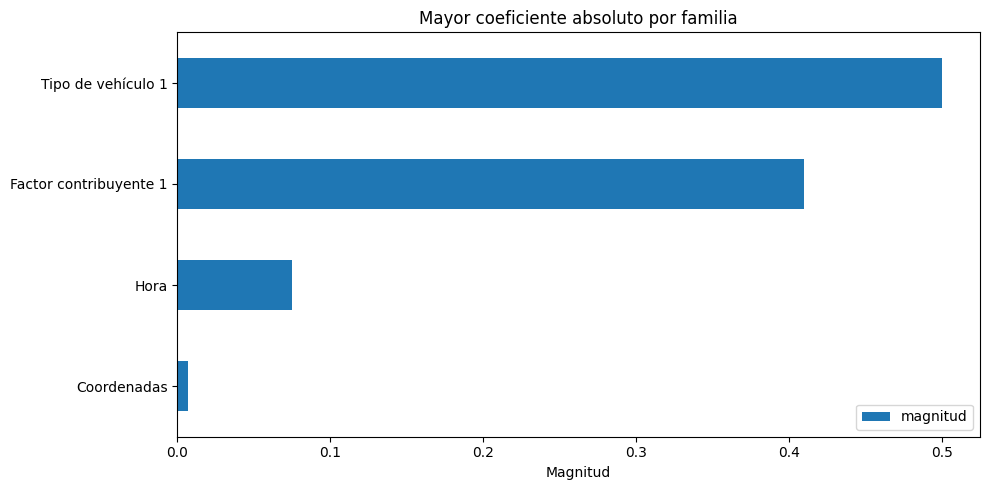
\includegraphics[width=0.82\textwidth]{imagenes/fig_cell_71_1.png}
    \caption{Comparación de la mayor magnitud absoluta de coeficiente ($|\beta_j|$) por familia de variables en la Regresión Logística.}
    \label{fig:q8_coeficientes}
\end{figure}

\noindent \textbf{Interpretación para la Pregunta 8 y punto de contacto con el negocio:}
Las familias categóricas de \textbf{Tipo de vehículo 1 ($|\beta|_{\max} = 0.5000$)} y \textbf{Factor contribuyente 1 ($|\beta|_{\max} = 0.4098$)} concentran el mayor peso discriminativo del modelo lineal, seguidas por la componente nocturna de la hora (\texttt{hora\_coseno}, $+0.0752$, que toma sus valores máximos positivos en las horas cercanas a la medianoche y la madrugada) y las coordenadas continuas (\texttt{lat}, $+0.0070$). Por ejemplo, defectos de iluminación (\texttt{OTHER LIGHTING DEFECTS}, $\beta = +0.4098$) incrementan el puntaje de riesgo fatal, mientras que colisiones de unidades de emergencia (\texttt{AMBULANE}, $\beta = -0.5000$) suelen reportarse incluso en incidentes de baja energía cinética por protocolo administrativo. Al mismo tiempo, la modesta capacidad predictiva global del modelo lineal ($\text{AUROC} = 0.5397$) demuestra dos realidades críticas para los tomadores de decisiones: (i) una combinación puramente lineal no captura las interacciones cruzadas entre hora, zona y vehículo (lo que motiva la implementación de la Red Neuronal Profunda en la Sección \ref{sec:bono_dl}, que eleva el AUROC a $0.6020$), y (ii) el formulario policial MV-104AN carece de variables cinemáticas directas como la velocidad estimada de impacto, el uso de cinturón/casco o el ancho de la vía.

\subsubsection{Evaluación Paramétrica del Modelo No Supervisado (K-Means)}

Sobre las $699$ cuadrículas urbanas activas ($\ge 10$ colisiones en el primer semestre de 2026) estandarizadas con \texttt{StandardScaler}, se ejecutó el algoritmo \texttt{KMeans} de MLlib (\texttt{seed=42}) probando tres valores del hiperparámetro $k \in \{2, 3, 4\}$ y evaluando la cohesión y separación de los grupos mediante el \textbf{coeficiente de Silhouette} con medida de distancia euclídea al cuadrado (\texttt{ClusteringEvaluator}).

\begin{table}[H]
\centering
\small
\renewcommand{\arraystretch}{1.2}
\caption{Evaluación del hiperparámetro $k$ en K-Means mediante el coeficiente de Silhouette en Spark MLlib.}
\label{tab:kmeans_silhouette}
\begin{tabular}{c c r}
\toprule
\textbf{Número de clústeres ($k$)} & \textbf{Medida de distancia} & \textbf{Coeficiente de Silhouette} \\
\midrule
$\mathbf{2}$ & \textbf{Euclídea al cuadrado (\texttt{squaredEuclidean})} & $\mathbf{0.473409}$ \\
$3$ & Euclídea al cuadrado (\texttt{squaredEuclidean}) & $0.459737$ \\
$4$ & Euclídea al cuadrado (\texttt{squaredEuclidean}) & $0.369069$ \\
\bottomrule
\end{tabular}
\end{table}

La configuración óptima corresponde a \textbf{$k = 2$ grupos ($\text{Silhouette} = 0.4734$)}, seguida de cerca por $k = 3$ ($0.4597$), mientras que $k = 4$ fragmenta excesivamente el espacio ($0.3691$). La Tabla \ref{tab:kmeans_perfiles} presenta los promedios de cada grupo reexpresados en sus unidades originales de negocio, y la Figura \ref{fig:kmeans_mapa} muestra su distribución geográfica sobre el mapa de Nueva York.

\begin{table}[H]
\centering
\scriptsize
\renewcommand{\arraystretch}{1.25}
\caption{Caracterización de los perfiles territoriales identificados por K-Means ($k=2$) en unidades originales (2026-I).}
\label{tab:kmeans_perfiles}
\setlength{\tabcolsep}{4pt}
\begin{tabularx}{\linewidth}{l c r r r r r X}
\toprule
\textbf{Clúster} & \textbf{Zonas} & \textbf{Colis.} & \textbf{Arrestos} & \textbf{Fatales} & \textbf{Noct.} & \textbf{Vuln.} & \textbf{Perfil territorial de negocio} \\
\midrule
\textbf{Grupo 0} & 351 & \textbf{83.815} & \textbf{365.991} & \textbf{0.171} & 20.3\% & \textbf{17.3\%} & \textbf{Zonas críticas de alta densidad e interacción vulnerable} (corredores centrales de Manhattan, Brooklyn, Bronx y ejes de Queens). \\
\textbf{Grupo 1} & 348 & 29.296 & 35.330 & 0.101 & 21.0\% & 8.7\% & \textbf{Zonas periféricas y residenciales de baja carga dual} (Staten Island, este de Queens y bordes costeros). \\
\bottomrule
\end{tabularx}
\end{table}

\begin{figure}[H]
    \centering
    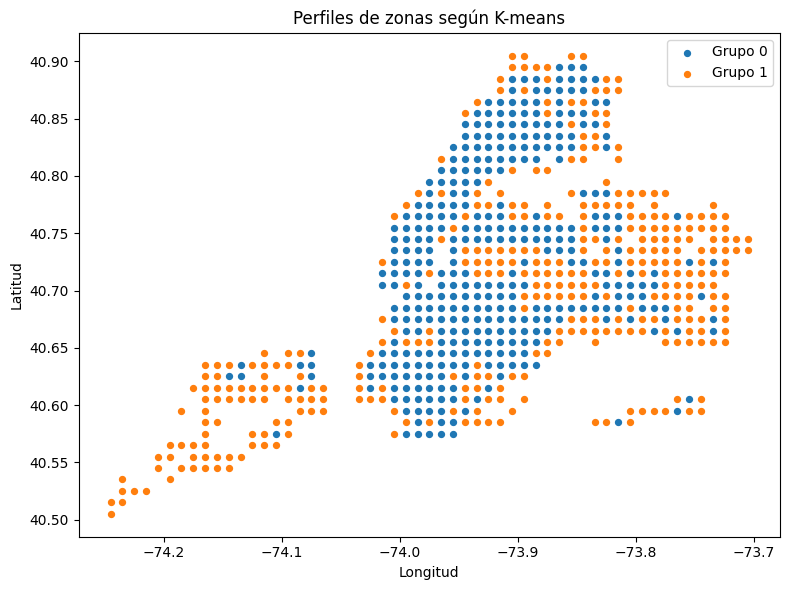
\includegraphics[width=0.76\textwidth]{imagenes/fig_cell_74_1.png}
    \caption{Distribución espacial de las 699 cuadrículas urbanas de Nueva York según los perfiles territoriales del modelo K-Means ($k=2$).}
    \label{fig:kmeans_mapa}
\end{figure}

\noindent \textbf{Interpretación de los perfiles K-Means para la toma de decisiones:}
El agrupamiento divide casi en dos mitades exactas las cuadrículas activas de la ciudad, pero con una asimetría operativa dramática:
\begin{itemize}
    \item \textbf{Grupo 0 ($351$ zonas --- Prioridad Operativa Alta):} Promedia \textbf{$83.8$ colisiones y $366.0$ arrestos por cuadrícula} (más de $10$ veces el volumen de arrestos del Grupo 1 y casi $3$ veces su volumen de colisiones), registra un $69\%$ más de colisiones fatales promedio ($0.171$ vs. $0.101$) y \textbf{duplica exactamente la proporción de choques con peatones o ciclistas heridos o fallecidos ($17.3\%$ frente a $8.7\%$)}. Espacialmente (Figura \ref{fig:kmeans_mapa}, puntos azules), conforma un corredor continuo que abarca Manhattan, el oeste y centro de Brooklyn, el sur y centro del Bronx y el eje central de Queens.
    \item \textbf{Grupo 1 ($348$ zonas --- Prioridad Preventiva y Vial Suburbana):} Promedia $29.3$ colisiones y $35.3$ arrestos por zona, con baja proporción de peatones/ciclistas afectados ($8.7\%$) pero una proporción de siniestralidad nocturna ligeramente superior ($21.0\%$ vs. $20.3\%$). Espacialmente (puntos naranjas), cubre Staten Island, el oriente de Queens y sectores periféricos de Brooklyn y el Bronx, donde predominan desplazamientos en automóvil particular y autopistas periféricas.
\end{itemize}


\section{Bono: Modelo de Aprendizaje Profundo en Spark MLlib}
\label{sec:bono_dl}

Como extensión avanzada del ejercicio de modelado supervisado, se implementó una red neuronal artificial profunda de propagación hacia adelante (\textit{Feedforward Deep Neural Network} / Perceptrón Multicapa) utilizando la clase distribuida \texttt{MultilayerPerceptronClassifier} de \textbf{Spark MLlib}, ejecutada íntegramente sobre el clúster \texttt{spark://10.195.34.34:7077}.

\subsection{Selección y Justificación frente al Modelo Lineal}
\label{subsec:bono_dl_seleccion}

El modelo se aplicó exactamente a la misma tarea predictiva de la Pregunta 8: estimar si una colisión vehicular registrada resulta en al menos una persona fallecida ($\texttt{label} \in \{0, 1\}$). A diferencia de la Regresión Logística evaluada en la Sección \ref{sec:modelado_evaluacion}, que combina las características de forma estrictamente aditiva y lineal en el logit, una red neuronal con múltiples capas ocultas y funciones de activación no lineales (sigmoide en las capas ocultas y \textit{softmax} en la capa de salida) es capaz de aprender automáticamente \textbf{interacciones de orden superior} entre la hora cíclica del día, la ubicación geográfica, la tipología del vehículo y el factor contribuyente (por ejemplo, combinaciones específicas donde cierto tipo de vehículo pesado solo incrementa drásticamente la letalidad en determinadas franjas nocturnas o corredores viales).

Para garantizar una comparación científica estrictamente justa frente a la Regresión Logística, el Perceptrón Multicapa utilizó las mismas $347$ variables de entrada generadas por el pipeline de preprocesamiento (\texttt{preparacion\_lr}), la misma partición temporal (2024 para entrenamiento, 2025 para validación y primer semestre de 2026 para prueba) y las mismas métricas de evaluación (\textbf{AUPRC}, \textbf{AUROC}, \textbf{Precisión}, \textbf{Exhaustividad} y \textbf{F1}).

\subsection{Preparación Distribuida y Diseño del Experimento de Hiperparámetros}
\label{subsec:bono_dl_experimento}

Dado que la implementación de \texttt{MultilayerPerceptronClassifier} en Spark MLlib no admite una columna de pesos por registro (\texttt{weightCol}), el desbalance extremo de clases en el conjunto de entrenamiento ($219$ colisiones fatales frente a $83,479$ no fatales) se compensó mediante sobremuestreo distribuido exacto en PySpark (\texttt{F.explode(F.sequence(...))}): cada registro fatal del conjunto de entrenamiento (2024) se replicó $381$ veces (equivalente al factor de ponderación $w_1 = 83{,}479 / 219 \approx 381.18$ empleado en la Regresión Logística), conformando un conjunto balanceado de entrenamiento con $83,479$ registros no fatales y $83,439$ registros fatales replicados, reparticionado en el clúster. Los conjuntos de validación (2025) y prueba (2026-I) se conservaron intactos sin réplicas.

Se diseñó una grilla experimental de \textbf{seis configuraciones} combinando tres arquitecturas de capas ocultas (con capa de entrada de $347$ neuronas y capa de salida de $2$ neuronas) y dos regímenes de iteraciones máximas del optimizador cuasi-Newton distribuido \textbf{L-BFGS} (\texttt{blockSize=256, seed=42}):
\begin{itemize}
    \item \textbf{Arquitectura 1 (2 capas ocultas):} $[347, 32, 16, 2]$ con $\texttt{maxIter} \in \{50, 150\}$.
    \item \textbf{Arquitectura 2 (2 capas ocultas de mayor anchura):} $[347, 64, 32, 2]$ con $\texttt{maxIter} \in \{50, 150\}$.
    \item \textbf{Arquitectura 3 (3 capas ocultas profundas en embudo):} $[347, 64, 32, 16, 2]$ con $\texttt{maxIter} \in \{50, 150\}$.
\end{itemize}

La Tabla \ref{tab:mlp_validacion} y la Figura \ref{fig:mlp_validacion} presentan el desempeño obtenido por las seis configuraciones sobre el conjunto de validación (año 2025).

\begin{table}[H]
\centering
\scriptsize
\renewcommand{\arraystretch}{1.2}
\caption{Resultados en el conjunto de validación (2025) por arquitectura de red neuronal y número de iteraciones L-BFGS.}
\label{tab:mlp_validacion}
\resizebox{\textwidth}{!}{%
\begin{tabular}{l c c r r}
\toprule
\textbf{Arquitectura de capas ocultas} & \textbf{Topología completa (\texttt{layers})} & \textbf{Iteraciones (\texttt{maxIter})} & \textbf{AUPRC validación} & \textbf{AUROC validación} \\
\midrule
2 capas (32--16) & $[347, 32, 16, 2]$ & 50 & $0.00412$ & $0.6181$ \\
2 capas (32--16) & $[347, 32, 16, 2]$ & 150 & $0.00331$ & $0.5651$ \\
2 capas (64--32) & $[347, 64, 32, 2]$ & 50 & $0.00391$ & $0.6251$ \\
2 capas (64--32) & $[347, 64, 32, 2]$ & 150 & $0.00274$ & $0.5802$ \\
\textbf{3 capas (64--32--16)} & $\mathbf{[347, 64, 32, 16, 2]}$ & $\mathbf{50}$ & $\mathbf{0.00721}$ & $\mathbf{0.7052}$ \\
3 capas (64--32--16) & $[347, 64, 32, 16, 2]$ & 150 & $0.00346$ & $0.6031$ \\
\bottomrule
\end{tabular}%
}
\end{table}

\begin{figure}[H]
    \centering
    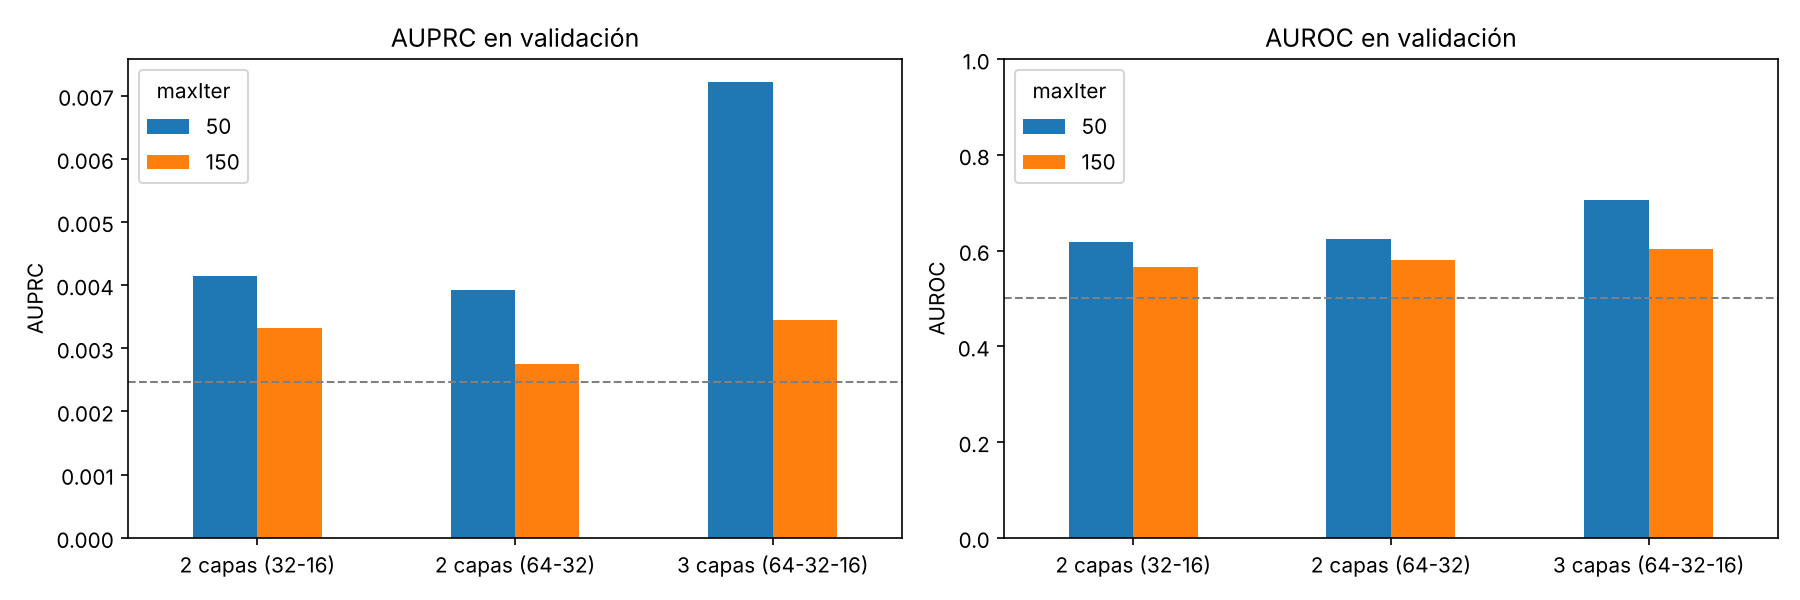
\includegraphics[width=0.95\textwidth]{imagenes/fig_mlp_validacion.png}
    \caption{AUPRC y AUROC en validación (2025) por arquitectura y número de iteraciones. La línea punteada indica la prevalencia base (izquierda) y el nivel de azar $0.5$ (derecha).}
    \label{fig:mlp_validacion}
\end{figure}

\noindent \textbf{Análisis del comportamiento en validación (efecto de parada temprana):}
La arquitectura más profunda de \textbf{tres capas ocultas ($64\text{--}32\text{--}16$) con $50$ iteraciones} alcanzó el mejor desempeño tanto en AUPRC ($0.00721$, casi tres veces la prevalencia base) como en AUROC ($0.7052$). Un hallazgo experimental muy relevante es que, en las tres arquitecturas evaluadas, aumentar las iteraciones de $50$ a $150$ degradó sistemáticamente las métricas de validación: dado que los $219$ casos fatales fueron replicados $381$ veces para equilibrar las clases, prolongar la optimización L-BFGS hace que la red memorice los ejemplos positivos replicados (\textit{overfitting}) y pierda capacidad de generalización sobre el año siguiente. En consecuencia, limitar el entrenamiento a $50$ iteraciones actúa como un mecanismo efectivo de regularización por parada temprana (\textit{early stopping}). Al calibrar el umbral de decisión sobre validación para la red $64\text{--}32\text{--}16$ ($\texttt{maxIter}=50$), el puntaje F1 se maximizó en $\tau = 0.85$.

\subsection{Evaluación Comparativa en Prueba frente a la Regresión Logística}
\label{subsec:bono_dl_comparacion}

La Tabla \ref{tab:mlp_vs_lr_test} y la Figura \ref{fig:mlp_vs_lr_test} comparan el desempeño de la Regresión Logística ($\texttt{regParam}=1.00, \tau=0.55$) y de la Red Neuronal Profunda MLP ($64\text{--}32\text{--}16, \texttt{maxIter}=50, \tau=0.85$) sobre el conjunto de prueba independiente del primer semestre de 2026 ($40,373$ colisiones, $102$ fatales, prevalencia del $0.25\%$).

\begin{table}[H]
\centering
\scriptsize
\renewcommand{\arraystretch}{1.25}
\caption{Comparación en el conjunto de prueba temporal (primer semestre de 2026, prevalencia de $0.25\%$) entre la Regresión Logística y la Red Neuronal Profunda (MLP).}
\label{tab:mlp_vs_lr_test}
\resizebox{\textwidth}{!}{%
\begin{tabular}{l c r r c r r r r}
\toprule
\textbf{Modelo en Spark MLlib} & \textbf{Umbral ($\tau$)} & \textbf{AUPRC} & \textbf{AUROC} & \textbf{Fatales detectadas} & \textbf{Falsos positivos} & \textbf{Precisión} & \textbf{Exhaustividad} & \textbf{F1} \\
\midrule
Regresión Logística & $0.55$ & $0.0042$ & $0.5397$ & $50\text{ de }102$ & $16,382$ & $0.30\%$ & $\mathbf{49.02\%}$ & $0.0060$ \\
\textbf{Red Neuronal (MLP 64--32--16)} & $\mathbf{0.85}$ & $\mathbf{0.0044}$ & $\mathbf{0.6020}$ & $23\text{ de }102$ & $\mathbf{5,934}$ & $\mathbf{0.39\%}$ & $22.55\%$ & $\mathbf{0.0076}$ \\
\bottomrule
\end{tabular}%
}
\end{table}

\begin{figure}[H]
    \centering
    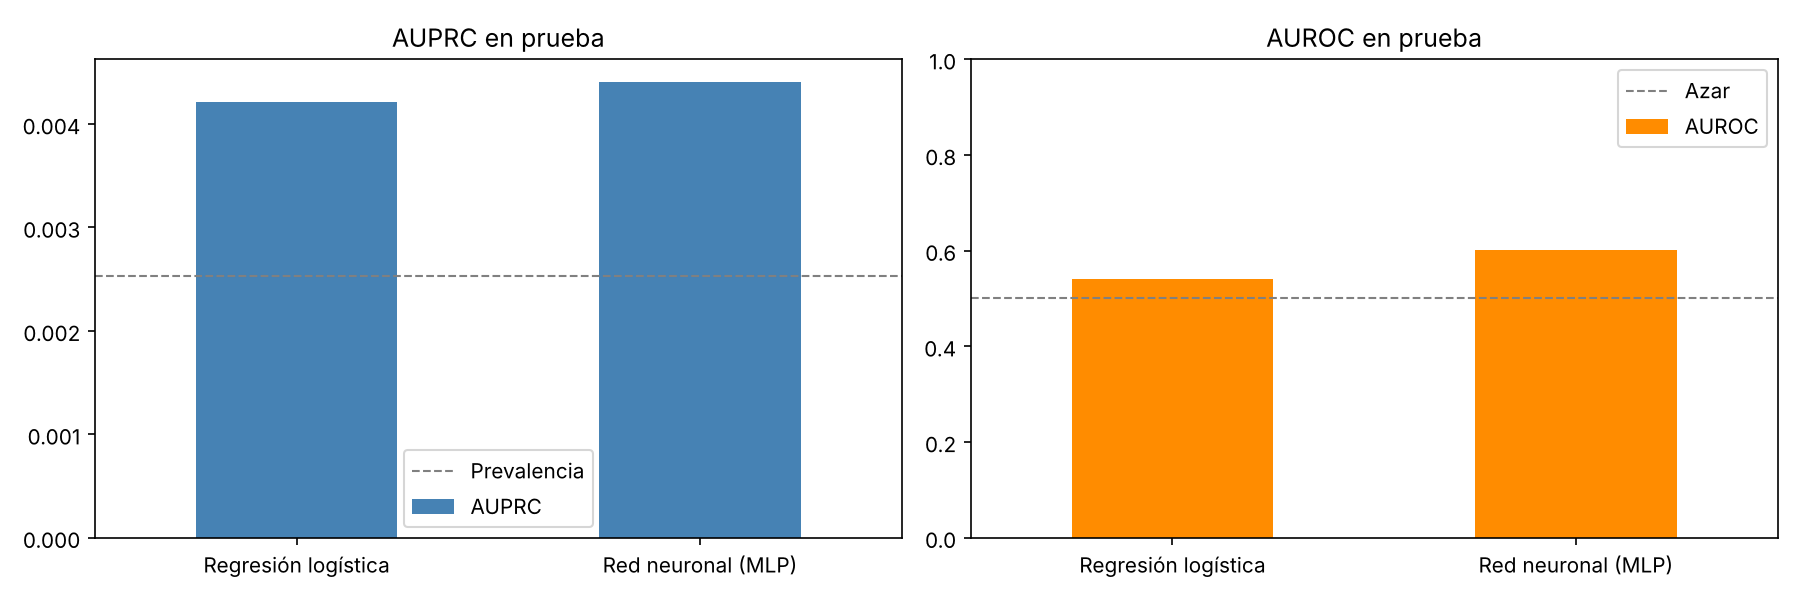
\includegraphics[width=0.95\textwidth]{imagenes/fig_mlp_vs_logistica.png}
    \caption{Comparación de AUPRC (izquierda) y AUROC (derecha) en el conjunto de prueba (2026-I) entre la Regresión Logística y la Red Neuronal (MLP).}
    \label{fig:mlp_vs_lr_test}
\end{figure}

\noindent \textbf{Conclusión del experimento de Aprendizaje Profundo:}
El Perceptrón Multicapa ordenó significativamente mejor las colisiones según su nivel de riesgo letal, elevando el \textbf{AUROC en prueba de $0.5397$ a $0.6020$ ($+6.23$ puntos porcentuales)}, mejorando la \textbf{AUPRC a $0.0044$}, incrementando la \textbf{precisión en un $30\%$ relativo ($0.39\%$ vs. $0.30\%$)} y alcanzando un mayor \textbf{F1 ($0.0076$ vs. $0.0060$)}. Con su umbral calibrado ($\tau = 0.85$), la red neuronal redujo en un \textbf{$63.8\%$ las falsas alarmas} ($5,934$ falsos positivos frente a $16,382$ de la Regresión Logística), a cambio de una menor exhaustividad puntual ($22.55\%$). Esto confirma empíricamente que existen interacciones no lineales entre hora, coordenadas, vehículo y factor contribuyente que las capas ocultas logran extraer, si bien para un sistema de despacho automático de emergencias en tiempo real sería indispensable enriquecer los registros del NYPD/DOT con variables cinemáticas de velocidad e infraestructura vial.


\section{Conclusiones y Recomendaciones Ejecutivas para Nueva York}
\label{sec:conclusiones_recomendaciones}

Al culminar las seis fases de la metodología \textbf{CRISP-DM} sobre el clúster de \textbf{Apache Spark} (\texttt{spark://10.195.34.34:7077}) y \textbf{Hadoop HDFS} (\texttt{hdfs://10.195.34.34:9000}), el equipo consultor presenta a los tomadores de decisiones del Estado y la Alcaldía de Nueva York las conclusiones estratégicas y el plan de acción respaldado por los hallazgos empíricos del proyecto:

\subsection{Síntesis de Hallazgos Estratégicos}

\begin{enumerate}
    \item \textbf{La estandarización poblacional transforma el mapa de prioridades de seguridad pública:}
    Analizar únicamente conteos absolutos distorsiona la asignación de recursos hacia Brooklyn ($42,877$ arrestos). Al normalizar mediante los pesos muestrales \texttt{PWGTP} de \textit{NYCgov Poverty Measure}, \textbf{El Bronx emerge como el condado con mayor presión per cápita de detenciones ($2,354.5$ arrestos Totales y $1,388.1$ por delitos menores por cada $100,000$ habitantes)}, coincidiendo con la tasa más alta de pobreza ponderada ($27.12\%$) y de desempleo civil ($9.56\%$) de la metrópoli.

    \item \textbf{Los arrestos por delitos graves (\textit{Felonies}) siguen un ciclo intrasemanal altamente concentrado entre martes y jueves:}
    Sobre los $55,651$ arrestos por felonías del primer semestre de 2026, más del $53\%$ ocurre exclusivamente entre martes y jueves ($29,540$ detenciones), con un desfase territorial claro del día pico: martes en el Bronx ($18.85\%$), miércoles en Brooklyn ($18.14\%$) y Queens ($18.84\%$), y jueves en Manhattan ($18.28\%$) y Staten Island ($18.10\%$).

    \item \textbf{Los peatones aportan casi la mitad de las muertes viales y las SUV lideran los siniestros contra vulnerables:}
    Sobre el histórico depurado de $2,305,355$ colisiones ($779,372$ heridos y $3,746$ fallecidos), los peatones representan el $49.3\%$ de todas las víctimas fatales ($1,847$ fallecidos). En el primer semestre de 2026, la distracción del conductor ($1,686$ choques) y no ceder el paso ($1,243$) fueron los principales factores en siniestros con peatones y ciclistas, mientras que las camionetas SUV (\texttt{STATION WAGON/SPORT UTILITY VEHICLE}, $1,741$) superaron a los sedanes ($1,554$) como el vehículo más involucrado.

    \item \textbf{Identificación microterritorial de 5 ``Zonas Calientes Duales'' y 2 Perfiles K-Means:}
    El cruce espacial en cuadrículas de $0.01^\circ \times 0.01^\circ$ identificó cinco zonas críticas donde convergen el máximo percentil de arrestos y colisiones mortales, encabezadas por \textbf{Bronx Central} $(40.845^\circ, -73.905^\circ)$ con $1,584$ arrestos y $2$ colisiones fatales ($\text{índice} = 0.9674$) y \textbf{Brooklyn Este} $(40.675^\circ, -73.905^\circ)$ con $1,107$ arrestos y $2$ colisiones fatales ($\text{índice} = 0.9511$). Complementariamente, el modelo \textbf{K-Means ($k=2, \text{Silhouette}=0.4734$)} segmentó las $699$ zonas activas de la ciudad en un \textbf{Grupo 0 de alta prioridad ($351$ zonas)} que concentra $10.4$ veces más arrestos promedio ($366.0$ vs. $35.3$) y el doble de afectación a peatones y ciclistas ($17.3\%$ vs. $8.7\%$) que el \textbf{Grupo 1 ($348$ zonas)}.

    \item \textbf{Superioridad de arquitecturas no lineales (MLP) sobre modelos lineales para modelar el riesgo fatal:}
    Mientras que la Regresión Logística ponderada ($\texttt{regParam}=1.00$) alcanzó una $\text{AUROC} = 0.5397$ en la prueba temporal de 2026 e identificó la alta influencia relativa de defectos de iluminación vial ($\beta = +0.4098$) y de la franja nocturna, el \textbf{Perceptrón Multicapa de tres capas ocultas ($64\text{--}32\text{--}16$, $\texttt{maxIter}=50$)} elevó la discriminación a $\text{AUROC} = 0.6020$ y redujo en un $63.8\%$ los falsos positivos, demostrando el valor de capturar interacciones espacio-temporales no lineales en \textbf{Spark MLlib}.
\end{enumerate}

\subsection{Hoja de Ruta y Recomendaciones para los Tomadores de Decisiones}

Con base en los hallazgos anteriores y cerrando la sexta fase (Despliegue) de la metodología CRISP-DM, la Tabla \ref{tab:recomendaciones_ejecutivas} estructura el plan de acción interinstitucional propuesto para la Alcaldía de Nueva York, articulando las intervenciones del NYPD, el NYC DOT (\textit{Vision Zero}), \textit{NYC Opportunity} y el Departamento de Salud estatal.

\begin{table}[H]
\centering
\scriptsize
\renewcommand{\arraystretch}{1.3}
\caption{Plan de acción interinstitucional recomendado para la Alcaldía y el Estado de Nueva York.}
\label{tab:recomendaciones_ejecutivas}
\begin{tabularx}{\linewidth}{>{\raggedright\arraybackslash}p{2.7cm} >{\raggedright\arraybackslash}p{3.4cm} X}
\toprule
\textbf{Entidad Responsable} & \textbf{Eje de Intervención} & \textbf{Acción Concreta Basada en la Evidencia del Proyecto} \\
\midrule
\textbf{Alcaldía de NYC / NYPD + NYC DOT} & Intervención conjunta en las 5 Zonas Calientes Duales y Clúster 0 & Priorizar inversión integrada (modernización de alumbrado público, atendiendo el coeficiente $+0.4098$ de \texttt{OTHER LIGHTING DEFECTS}, cámaras de control y patrullaje) en las cuadrículas $(40.845^\circ, -73.905^\circ)$ en el Bronx y $(40.675^\circ, -73.905^\circ)$ en Brooklyn, así como en las $351$ celdas del \textbf{Grupo 0 de K-Means}. \\
\textbf{NYPD (\textit{CompStat})} & Reprogramación dinámica semanal por condado & Escalonar los turnos de unidades tácticas y cumplimiento judicial entre martes y jueves ($53.1\%$ de las felonías): refuerzo los martes en el Bronx (precintos 40, 44, 46, 47, 52), miércoles en Brooklyn y Queens (precintos 73, 75, 103, 110) y jueves en Manhattan (precinto 14). \\
\textbf{NYC DOT (\textit{Vision Zero})} & Protección de vulnerables y gestión horaria asimétrica & Instalar intervalos peatonales adelantados (LPI) y reductores de velocidad de giro en intersecciones del Clúster 0 para mitigar \texttt{FAILURE TO YIELD} ($1,243$ casos) y colisiones de SUV ($1,741$). Ajustar semáforos inteligentes en Staten Island a los picos pendulares de 07:00--08:00 h y 15:00 h, y en Manhattan a la meseta de 12:00--18:00 h y franja nocturna 21:00--01:00 h, intensificando campañas preventivas en meses cálidos ($r = +0.469$ entre temperatura y heridos). \\
\textbf{NYC Opportunity \& NYS Health} & Focalización social y enriquecimiento del registro MV-104AN & Sustituir enfoques puramente punitivos en delitos menores (\texttt{M}) del Bronx ($27.12\%$ pobreza, $9.56\%$ desempleo) por programas de empleo juvenil para el grupo etario 18--44 años, y fortalecer el tamizaje oncológico preventivo en los 3 PUMA de Staten Island ($514.7$ casos / 100k hab.). Incorporar en el formulario MV-104AN la velocidad límite de la vía y condiciones de iluminación para elevar el poder predictivo de los modelos de MLlib. \\
\bottomrule
\end{tabularx}
\end{table}


\newpage
% ==========================================
% REFERENCIAS BIBLIOGRÁFICAS
% ==========================================
\bibliographystyle{IEEEtran}
\bibliography{referencias}

\end{document}
